\documentclass[a4paper, 11pt]{article}

\usepackage{graphicx}
\usepackage{adjustbox}
\usepackage{subfigure}
\usepackage{amsmath}
\usepackage{color}
\usepackage[table]{xcolor}% http://ctan.org/pkg/xcolor
% Use symbols like degrees
\usepackage{textcomp, gensymb}
% In case we need to rotate a table
\usepackage{rotating}
% To insert code samples
\usepackage{listings}
\usepackage{caption}
\usepackage{xspace}
\usepackage{scrextend}
\usepackage{url}
\captionsetup[table]{skip=-10pt}

% To make interactive table of contents TODO: NOT WORKING FOR NOW, CHECK WHY
%\usepackage[dvipdfm]{hyperref}
\usepackage{hyperref}
\hypersetup{
    colorlinks=true,
    linkcolor=blue,
    urlcolor=magenta,
    linktoc=all
}

% Change margins because article class is too small
\addtolength{\oddsidemargin}{-2cm}
\addtolength{\evensidemargin}{12cm}
\addtolength{\textwidth}{4cm}
\addtolength{\topmargin}{-3cm}
\addtolength{\textheight}{5cm}

% define some colors here if needed
\definecolor{_green}{rgb}{0,0.6,0}
\definecolor{_gray}{rgb}{0.5,0.5,0.5}
\definecolor{_mauve}{rgb}{0.58,0,0.82}
\definecolor{_lyellow}{rgb}{0.1,0.1,0.1}

% code listing settings
\lstset{
  %rulecolor=\color{black},         % if not set, the frame-color may be changed on line-breaks within not-black text (e.g. comments (green here))
  tabsize=2,	                   
  title=\lstname                    % show the filename of files included with \lstinputlisting; also try caption instead of title
  backgroundcolor=\color{white},  % choose the background color;
  language=C++,                     % the language of the code
  basicstyle=\ttfamily\small,       % the size of the fonts that are used for the code 
  aboveskip={1.0\baselineskip},
  belowskip={1.0\baselineskip},
  columns=fixed,
  extendedchars=true,               % lets you use non-ASCII characters; for 8-bits encodings only, does not work with UTF-8
  breaklines=true,                  % sets automatic line breaking
  tabsize=4,                        % sets default tabsize to X spaces
  prebreak=\raisebox{0ex}[0ex][0ex]{\ensuremath{\hookleftarrow}},
  frame=lines,                      % adds a frame around the code (eg. single)
  showtabs=false,                   % show tabs within strings adding particular underscores
  showspaces=false,                 % show spaces everywhere adding particular underscores; it overrides 'showstringspaces'
  showstringspaces=false,           % underline spaces within strings only
  keywordstyle=\color{_mauve},      % keyword style
  commentstyle=\color{_green},      % comment style
  stringstyle=\color{_gray},        % string literal style
  deletekeywords={...},             % if you want to delete keywords from the given language
  otherkeywords={*,...},            % if you want to add more keywords to the set
  numbers=left,                     % where to put the line-numbers;
  keepspaces=true,                  % keeps spaces in text, useful for keeping indentation of code (possibly needs columns=flexible)
  numberstyle=\footnotesize\color{_gray},% the style that is used for the line-numbers 
  stepnumber=1,                     % the step between two line-numbers.
  numbersep=5pt,                    % how far the line-numbers are from the code
  captionpos=t,                     % sets the caption-position bottom(b), top(t)
  escapeinside={\%*}{*)}            % if you want to add LaTeX within your code
}

\newcommand{\castor}{\textsc{CASToR}\xspace}

% Uncomment for development version (SPECT)
% Comment for production version (PET only)
%\newcommand{\dev}{}

\begin{document}

% Title page
\title{Customizable and Advanced Software for Tomographic Reconstruction (CASToR)}
\author{Version 3.1}
\maketitle
\centerline{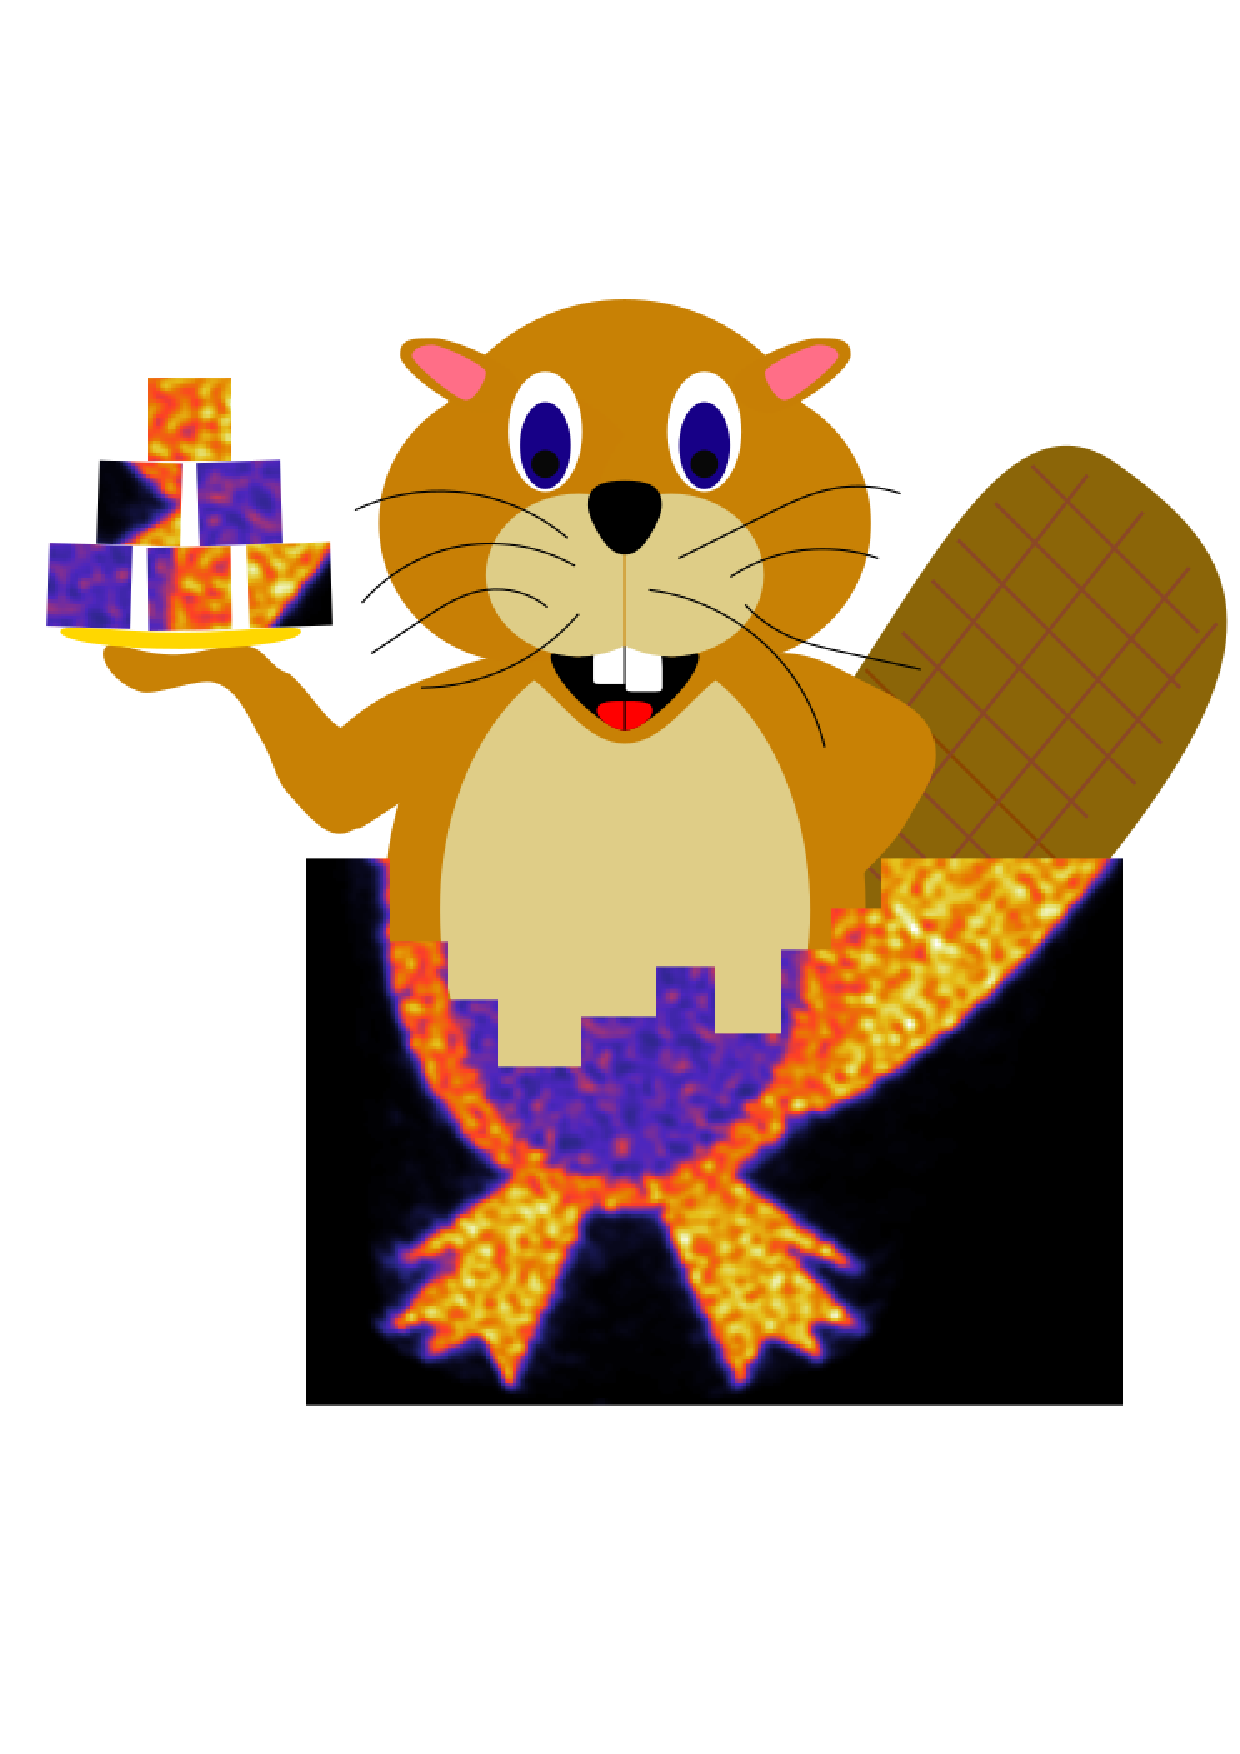
\includegraphics[scale=0.5]{figures/CASToR_logo.pdf}}
\newpage

% Table of contents
\tableofcontents


%---------------------------------------------------------------------------------------------------------------------------------------------------------------
%---------------------------------------------------------------------------------------------------------------------------------------------------------------
%---------------------------------------------------------------------------------------------------------------------------------------------------------------
%                S U M M A R Y
%---------------------------------------------------------------------------------------------------------------------------------------------------------------
%---------------------------------------------------------------------------------------------------------------------------------------------------------------
%---------------------------------------------------------------------------------------------------------------------------------------------------------------
\newpage
\section*{Summary}

This document is the main manual of the \castor software platform for tomographic image reconstruction.
It describes the general features of the platform and the scope of its applications.
The input datafile formats and the description of the scanner systems are also detailed in this document.
For developers, specific advanced manuals about different parts of the platform are available on the CASToR website.\\
\\
The manual contains the following sections:
\begin{itemize}
  \item Section \ref{s_features} presents the features implemented in the platform. 
  \item Section \ref{s_architecture} introduces \castor architecture and details some implementation issues. 
  \item Section \ref{s_install} describes how to install \castor for Unix and Windows systems.
  \item Section \ref{s_quickstart} contains some basic steps to start with \castor. 
  \item Section \ref{s_scanner_integration} describes PET, SPECT and CT systems definition in \castor and their integration to the platform.
  \item Input PET, SPECT and CT raw data and related metadata file formats used by \castor are specified in section \ref{s_input_files}. 
  \item Section \ref{s_interfile} describes the Interfile image format used by \castor.
  \item Section \ref{s_utilities} presents several toolkits related to \castor.
\end{itemize}


%---------------------------------------------------------------------------------------------------------------------------------------------------------------
%---------------------------------------------------------------------------------------------------------------------------------------------------------------
%---------------------------------------------------------------------------------------------------------------------------------------------------------------
%                C A S T O R   F E A T U R E S
%---------------------------------------------------------------------------------------------------------------------------------------------------------------
%---------------------------------------------------------------------------------------------------------------------------------------------------------------
%---------------------------------------------------------------------------------------------------------------------------------------------------------------
\newpage
\section{CASToR features}
\label{s_features}

The current version of \castor includes the following features:

\begin{itemize}
  \item Iterative reconstruction algorithms.
  \item PET, SPECT (parallel-hole and convergent-beam collimators) and CT (flat panel) geometries.
  \item Reconstruction of multi-frames and respiratory/cardiac gated acquisitions.
  \item Projector plug-in class system, including usual algorithms such as Siddon~\cite{Siddon}~\cite{FastSiddon}, Joseph~\cite{Joseph} and Distance-Driven~\cite{DistanceDriven} projectors.
  \item Reconstruction of TOF PET list-mode and histogrammed data.
  \item Optimisation algorithm plug-in class system, including most well-known algorithms such as MLEM~\cite{MLEM}, One-Step-Late~\cite{OSL} and MLTR~\cite{MLTR} optimization, and also many others.
  \item Plug-in class systems for image convolution and general image processing.
  \item Two-level parallel CPU implementation using MPI (multi-computers) and openMP (multi-threads) libraries.
  \item Interfile I/O format for images.
  \item Utility tool to convert GATE~\cite{GATE} Monte Carlo simulated data in ROOT format~\cite{ROOT} into the \castor datafile format.
\end{itemize}

A list of all features can be found on the website (see \url{http://www.castor-project.org/features}).

Several advanced manuals dedicated to specific parts of the code as well as a Doxygen documentation are also available for developers (see \url{http://www.castor-project.org/documentation}).


%---------------------------------------------------------------------------------------------------------------------------------------------------------------
%---------------------------------------------------------------------------------------------------------------------------------------------------------------
%---------------------------------------------------------------------------------------------------------------------------------------------------------------
%                C A S T O R   A R C H I T E C T U R E
%---------------------------------------------------------------------------------------------------------------------------------------------------------------
%---------------------------------------------------------------------------------------------------------------------------------------------------------------
%---------------------------------------------------------------------------------------------------------------------------------------------------------------
\newpage
\section{CASToR architecture}
\label{s_architecture}

The \castor platform is an open-source software for tomographic image reconstruction, written in C++11.
The key points of \castor are generic programming, flexibility, and modularity. 
The code is segmented in several main components including data files management, image processing, optimization algorithms, projectors. 
To make the code generic and modular, specific classes implementing specific features in a component, inherit from an abstract class. 
Most of the code is implemented in the abstract classes so that the development of specific classes in the most comprehensive way requires
the minimum amount of code. 
Following these guidelines, rather than implementing the different file formats specific to the scanner manufacturers, \castor uses unified
file formats for the scanner descriptions (see section~\ref{s_scanner_integration}), and for the input data (see section~\ref{s_input_files}).
This allows a unique implementation of the core of the reconstruction algorithms, without having to distinguish between a set of particular
cases.
The distinctions between the modalities (PET, SPECT or CT), the types of data (list-mode or histogram) and the scanner manufacturers do not appear
in the core algorithm.
They are specified in the input data files and in the scanner description.
This results in a few blocks of code specific to a scanner model or to a data type while keeping the rest of the code entirely generic.
This avoids the duplication of parts of the code and any new adds-on to the code will hence be available for multiple setups and configurations.
Based on this code design, all correction terms required for quantitative reconstruction have to be estimated outside \castor and
must be supplied in the input datafile. 
This includes the normalization factors, the scattered events distribution, the random coincidences distribution in PET, and the attenuation
coefficients in emission tomography. 
Finally, genericity  being often a source of inefficiency, special care has been taken to optimize as much as possible the code
efficiency. 
The software has two levels of parallelism: a high-level splitting of the data using  MPI (Message Passing Interface) and a low-level
multi-threading of the loops over the events using the OpenMP (Open Multi-Processing) API.
\\
Being generic requires a clear definition of all the concepts involved in tomographic reconstruction.
For clarification, the definition of some of the terms and concepts used in \castor are given below.

\begin{itemize}

  \item An \textit{algorithm} is the mathematical method used to solve a problem, like an inverse problem in tomographic image reconstruction.
        An \textit{algorithm} can be analytical, iterative (in the sense of optimization), or of any other kind (SVD, posterior estimation,
        \textit{etc}). Currently, the \castor implementation considers only iterative optimization algorithms.

  \item In emission or transmission tomography, the data can be recorded in \textit{list-mode} or \textit{histogram} formats. 
        In \castor, whatever the data format, a \textit{datafile} is defined as being a collection of \textit{events}. 
        There are currently six different types of events implemented in \castor: PET histogram event, PET list-mode event, PET normalization event, SPECT histogram event, SPECT list-mode event and CT histogram event.
        A list-mode event corresponds to the detection of one single photon or one coincidence.
        A histogram event corresponds to the data acquired during a given time frame in a given detection element, eventually for a given synchronization gate.
        A normalization event corresponds to a normalization factor and an attenuation correction factor associated to a list of data channels.
        An example of PET histogram event is the number of detected coincidences for a given pair of crystals in coincidence.

  \item A \textit{datafile} is linked to a given \textit{scanner} geometry. 
        A \textit{scanner} in \castor can be described either by the geometry of a physical scanner (\textit{e.g.} a collection of individual
        crystals arranged in a ring geometry for a cylindrical PET system) or by a generic \textit{sinogram} geometry. 
        In \castor, the word \textit{sinogram} is not used for a \textit{datafile} format, but for the geometrical organization of the data
        in a discretized four-dimension projection space.
        Each \textit{event} attached to a \textit{sinogram} geometry corresponds to a specific projection line expressed by the standard 4-D sinogram
        coordinates: a radial position, an azimuthal angle, an axial position, and co-polar angle.
        On the other hand, each \textit{event} attached to a physical PET scanner geometry corresponds to a specific pair of crystals in coincidence,
        or a group of crystal pairs in case of angular mashing or axial compression. 
        As a consequence, both a PET histogram and a PET list-mode \textit{event} can be attached to a \textit{sinogram} geometry or a physical scanner geometry.
        Currently, \castor implements only physical PET, SPECT (for parallel hole and convergent-beam collimators) and CT (flat panel) scanners geometries.
        The implementation of the \textit{sinogram} scanner geometry is planned for future releases.

  \item Tomographic image reconstruction consists in the inversion of the data model linking the data space to the image space. 
        Aside from the additive background in the detected events (scattered events and random coincidences in PET), this model is based on the so-called
        \textit{projector}. 
        In \castor, the task of the \textit{projector} is only to compute the system matrix elements corresponding to a given \textit{event}, that is one
        row of the system matrix. 
        The \textit{projector} does not perform the forward or backward projections; they are computed inside the \textit{algorithm}.

\end{itemize}

There are also general concepts that apply only to specific types of algorithms. 
The following subsections provide information for these different types of algorithms.

%---------------------------------------------------------------------------------------------------------------------------------------------------------------
%---------------------------------------------------------------------------------------------------------------------------------------------------------------
\subsection{Iterative optimization algorithms}

\begin{itemize}

  \item Iterative optimization algorithms (like ML-EM) are based on an objective function (\textit{Maximum Likelihood}, ML) and a iterative mechanism
        used to minimize or maximize this function(\textit{Expectation Maximization}, EM).
        The objective function is made of a data fidelity term and potentially a penalty term. 
        In \castor, the iterative optimization algorithm is generic: both the objective function and the iterative optimization are pulled into
        what we call an \textit{optimizer}. 
        Particular \textit{optimizers} can deal with \textit{penalties}, although they are not yet implemented. 
        For details about how the \textit{optimizer} is implemented in \castor, look at the \textit{CASToR\_HowTo\_optimizer\_and\_penalty} specific
        documentation (see \url{http://castor-project.org/documentation} ).

  \item For each iteration, and for each sub-iteration for optimization algorithms using ordered subsets of the data, a parallel loop over the
        \textit{events} is performed using OpenMP.
        For each \textit{event}, the following operations are performed:
        \begin{enumerate}
          \item The \textit{projector} is called to compute the corresponding system matrix elements, that is one row of the system matrix.
                If unmatched projectors are used, this operation is performed for both forward and backward projectors.
          \item The \textit{optimizer} is called to perform the \textit{data update step}. The following steps are performed: 
          \begin{enumerate}
            \item Forward projection of the current image estimate for the given row of the system matrix.
            \item Compute the foward mode: for emission, add any provided estimation of the additive background (scattered events and random coincidences) to the forward projection, or for transmission, apply the exponential to the forward projection, apply the blank estimation and add any additive background.
            \item Perform operations specific to the \textit{optimizer} to compute the correction term in the data space.
            \item Backward projection of the correction term in a back-projected correction image for the given row of the system matrix.
          \end{enumerate}
        \end{enumerate}
        Based on this strategy, when matched forward and backward projectors are used, the \textit{projector} is only called once. 
        As it is the most costly operation in tomographic reconstruction, significant acceleration factors can be therefore easily achieved. 
        Note that the \textit{optimizer} performs the forward and backward projections taking all system matrix multiplicative terms into account:
        calibration factor, decay factor, decay branching ratio, frame duration, normalization and attenuation factors.
        For SPECT, given an attenuation map and one row of the system matrix, a double loop is performed to take the attenuation into account.

  \item For optimization algorithms using ordered subsets, in each subset the main loop is performed over all $N_{\mathrm{Events}}$ events of the
        datafile, with an increment equal to the number of subsets $N_s$, starting at the event index $i_{\mathrm{event}}$ equal to the index $i_s$
        of the current subset: \[ {\mathrm{for}}(i_{\mathrm{event}}=i_s;i_{\mathrm{event}}<N_{\mathrm{Events}};i_{\mathrm{event}}+=N_s). \]
        Note that the number of subsets can be different for each iteration. 
        The same loop is used whatever the data type (list-mode or histogram) and modality. 
        Thus, when using subsets in the \textit{optimizer}, it is the user's responsibility to order the histogram events in an appropriate manner. 
        To avoid potential artifacts in the reconstructed image, {\color{red} we strongly discourage to write the histogram events with the inner
        loop over the radial or axial coordinate}. We recommend to randomly mix the order to the histogram events before writing them in the
        \textit{datafile} or, at least, to write the events with the inner loop over the azimuthal coordinate.

  \item Iterative optimization algorithms require the computation of a sensitivity image, requiring a backward projection step over all possible
        (empty or not) detection elements.
        When reconstructing histogram data, the sensitivity image is computed on-the-fly by the \textit{optimizer} for each subset. As the
        \textit{projector} is called only once, the cost of the backward projection associated to the sensitivity image computation is minimal. 
        It also allows to have a different number of subsets for each iteration. 
        Note that for some specific algorithms (\textit{e.g.} NEGML~\cite{NEGML}), the sensitivity images depend on the current image estimate.
        When reconstructing list-mode data, the sensitivity image is precomputed before launching the iterations.
        The loop over all possible detection elements is based either only on the characteristics of the scanner geometry description (thus ignoring
        normalization factors) or on a user's provided normalization datafile including the normalization factors (see section~\ref{s_input_files}).

\end{itemize}

%---------------------------------------------------------------------------------------------------------------------------------------------------------------
%---------------------------------------------------------------------------------------------------------------------------------------------------------------
\subsection{Analytical algorithms}

Analytical algorithms are not yet implemented into \castor.

%---------------------------------------------------------------------------------------------------------------------------------------------------------------
%---------------------------------------------------------------------------------------------------------------------------------------------------------------
\subsection{Other possible types of algorithms}

Other types of algorithms exist, but are not yet implemented into \castor.


%---------------------------------------------------------------------------------------------------------------------------------------------------------------
%---------------------------------------------------------------------------------------------------------------------------------------------------------------
%---------------------------------------------------------------------------------------------------------------------------------------------------------------
%                C A S T O R   I N S T A L L A T I O N
%---------------------------------------------------------------------------------------------------------------------------------------------------------------
%---------------------------------------------------------------------------------------------------------------------------------------------------------------
%---------------------------------------------------------------------------------------------------------------------------------------------------------------
\newpage
\section{CASToR installation}
\label{s_install}

CASToR source code is available on the CASToR website at castor-project.org, once you complete the short registration form (castor-project.org/form/castor-registration-form).
%If you have suscribed before the 1st version release and did not receive any email for some reason, just fill in the form once again to get access to the download link.
Do not hesitate to subscribe to the mailing-list in order to receive information about new versions of the platform and follow the CASToR community.
In addition, if you are interested in contributing as a developer in the \castor platform, please fill in the required fields in the subscription form.
Once the \castor collaboration will be ready to open the project for external contributions, you will be contacted with details on how to proceed.
In the meantime, if you already developed something that may be interesting for others, please let us know on the mailing list.

%---------------------------------------------------------------------------------------------------------------------------------------------------------------
%---------------------------------------------------------------------------------------------------------------------------------------------------------------
\subsection{Operating systems: 32 bits VS 64 bits}
\label{ss_install_os}

If run on 64 bits systems, any datafile can be read and used whatever its size, even if its size exceeds the size of the memory, thanks to datafile mapping.
However, if run on 32 bits systems, it is not possible to process datafiles bigger than 2 GB, whatever the size of the memory.

%---------------------------------------------------------------------------------------------------------------------------------------------------------------
%---------------------------------------------------------------------------------------------------------------------------------------------------------------
\subsection{Computation and data precision}
\label{ss_install_precision}

In CASToR, the precision of floating point numbers can be customized. This is implemented through the use of macro definitions interpreted by the pre-processor
of the compiler, defining the type of different variables throughout the code, as follows:

\begin{itemize}
  \item FLTNB: General floating-point precision (input/intermediary/output image matrices and some floating point operations).
  \item HPFLTNB: Higher floating-point precision for sensitive computations that require at least double precision (projector implementation, random number generators, \textit{etc}).
  \item FLTNBDATA: Precision of the floating point variables read or written into CASToR datafiles.
  \item FLTNBLUT: Precision of the floating point variables read or written into CASToR scanner LUT elements.
\end{itemize}

The types of these macros are defined in the \textit{include/management/gVariables.hh} and are all set to \textit{float} simple precision by default expect for HPFLTNB which is set to \textit{double} precision.
They can be changed to \textit{double} or \textit{long double} precision as desired, assuming that the operating system and the compiler are both able
to take these types into account (see \url{https://en.wikipedia.org/wiki/Long\_double}).
When any of these definitions is changed, the code needs to be entirely recompiled.
Note also that the memory requirements of the CASToR program will double with the use of \textit{double} precision compared to \textit{float} precision.

%---------------------------------------------------------------------------------------------------------------------------------------------------------------
%---------------------------------------------------------------------------------------------------------------------------------------------------------------
\subsection{CASToR configuration folder}
\label{ss_install_config}

The CASToR programs may use a bunch of configuration files, for scanners, default module's configurations, isotopes database, \textit{etc}. In the CASToR source
tree, there is a folder named \textit{config}, which contains all these configuration files. For instance, a datafile is linked to a scanner description;
this scanner description, either based on a geometrical file or a LUT file (see section~\ref{s_scanner_integration}), is located in the
\textit{config/scanner} sub-folder. There is also one sub-folder per type of modules (\textit{e.g.} projector, convolver, \textit{etc}). And finally, there is a
\textit{config/misc} folder containing miscellaneous configuration files, such as isotopes' database with their associated half-life and branching ratio.

When running CASToR, the configuration folder is localized by the \textit{CASTOR\_CONFIG} environment variable. If the code was compiled using the CMake
tools (see sub-sections~\ref{sss_install_unix_cmake} and \ref{sss_install_win_cmake}), this variable has been hard-linked to the executable during the
compilation. If the code was compiled using the provided Makefile (see sub-section~\ref{sss_install_unix_makefile}), this variable is read dynamically
from the \textit{CASTOR\_CONFIG} environment variable; so this variable must exist during run-time and point to the absolute path of the \textit{config}
directory. If the code is cross-compiled from a 64-bits Unix system for Windows systems (see sub-section~\ref{sss_install_win_cross}), then the environment
variable is also hard-linked during compilation. If the environment variable does not exist during the compilation, a compilation error will occur on purpose,
specifying that you must set it. Note that the value of this environment variable for cross-compilation should contain the path of the configuration folder
under the Windows system that will be used for execution. This path can use "/" instead of "\textbackslash" but must not be provided within "double quotes".
Finally, whatever the value of the \textit{CASTOR\_CONFIG} environment variable and whether it was hard-linked during the compilation or not, the path to
the configuration folder can be overloaded by using the \textit{-conf} command-line option.

%---------------------------------------------------------------------------------------------------------------------------------------------------------------
%---------------------------------------------------------------------------------------------------------------------------------------------------------------
\subsection{Unix systems}
\label{ss_install_unix}

There are two alternatives to compile the code: using the provided Makefile or the CMake tools.
If you do not link CASToR to external libraries, we recommend using the standard Makefile as it is quite straightforward.

%---------------------------------------------------------------------------------------------------------------------------------------------------------------
\subsubsection{Compile CASToR on Unix systems using the provided Makefile}
\label{sss_install_unix_makefile}

\begin{enumerate}
  \item Get the CASToR source code
  \item Configure the compilation using the following environment variables considered during the compilation (export CASTOR\_XXX = ):
  \begin{itemize}
    \item CASTOR\_CONFIG:  \textit{Set to the absolute path of the CASToR configuration directory (\textit{i.e.} the \textit{config} directory inside the source tree)}
    \item CASTOR\_MPI:     \textit{Set to 1 to build CASToR with MPI (required for multiprocessing / parallel computing at the datafile level)}
    \item CASTOR\_OMP:     \textit{Set to 1 to build CASToR with OpenMP (required for multithreading / parallel computing at the event level)}
    \item CASTOR\_ROOT:    \textit{Set to 1 to build CASToR with ROOT library (for datafile conversion using root. In case of issues with compilation using ROOT, check the \textit{root-config -libs} and \textit{root-config -cflags} variables are correctly initialized.)}
    \item CASTOR\_SIMD:    \textit{Set to 1 to build CASToR with SIMD optimization options from the compiler (CASToR does not include any specific vector programming)}
    \item CASTOR\_VERBOSE: \textit{Set to 1 to output maximum information during reconstruction, mainly used for debugging}
    \item CASTOR\_DEBUG:   \textit{Set to 1 to activate many additional checks inside primitive functions of the code, mainly used for debugging as it can slow down the execution}
  \end{itemize}
  \item Run \textit{make} to compile the CASToR code (you can use the '-j X' option of Makefile to use X threads during the compilation).
        It will create binaries for the main reconstruction program (castor-recon) and for each utility (section \ref{s_utilities}) into the \textit{bin} directory.
  \item (optional) Add CASToR to your environment using one of the following command lines: 

- bash or zsh:

\verb| export PATH=$PATH:/path/to/CASToR/bin|

- tcsh

\verb| setenv PATH ${PATH}:$/path/to/CASToR/bin|
\end{enumerate}

%---------------------------------------------------------------------------------------------------------------------------------------------------------------
\subsubsection{Compile CASToR on Unix systems using CMake}
\label{sss_install_unix_cmake}

\begin{enumerate}
  \item Install CMake: www.cmake.org
  \item Get the CASToR source code
  \item Configure the compilation using the following CMake variables:
  \begin{itemize}
    \item CASToR\_CONFIG:  \textit{Define the absolute path of the CASToR configuration directory (\textit{i.e.} the \textit{config} directory inside the source tree)}
    \item CASToR\_64bits:  \textit{Build CASToR on 64 bits architecture}
    \item CASToR\_ELASTIX: \textit{Build CASToR with Elastix (Deformation class using Elastix will be provided in further release)}
    \item CASToR\_MPI:     \textit{Build CASToR with MPI (required for multiprocessing / parallel computing at the datafile level)}
    \item CASToR\_OMP:     \textit{Build CASToR with OpenMP (required for multithreading / parallel computing at the event level)}
    \item CASToR\_ROOT:    \textit{Build CASToR with ROOT library (for datafile conversion using root)}
    \item CASToR\_SIMD:    \textit{Build CASToR with SIMD optimization options from the compiler (CASToR does not include any specific vector programming)}
    \item CASToR\_VERBOSE: \textit{Output maximum information during reconstruction, mainly used for debugging}
    \item CASToR\_DEBUG:   \textit{Activate many additional checks inside primitive functions of the code, mainly used for debugging as it can slow down the execution}
  \end{itemize}
  \item Run CMake for CASToR. It will create a makefile for your compiler.
  \item Run \textit{make} to compile the CASToR code (you can use the '-j X' option of Makefile to use X threads during the compilation).
        It will generate binaries for the main reconstruction program (\textit{castor-recon}) and for each utility (see section \ref{s_utilities}) into the \textit{bin} directory.
  \item (Facultative) Add CASToR to your environment using one of the following command lines: 

- bash or zsh:

\verb| export PATH=$PATH:/path/to/CASToR/bin|

- tcsh

\verb| setenv PATH ${PATH}:$/path/to/CASToR/bin|
\end{enumerate}

%---------------------------------------------------------------------------------------------------------------------------------------------------------------
%---------------------------------------------------------------------------------------------------------------------------------------------------------------
\subsection{Windows systems}
\label{ss_install_win}

% NOT RELEVANT ANYMORE Whatever the compilation method used, when executing CASToR on Windows systems, there may be some limits about the use of memory. In particular, due to the current implementation of the datafile read operations, some errors can appear above a certain amount of information read from the file. A workaround is to limit the size of the portion of the datafile that is loaded in memory by using the option \textit{-load}. The parameter of this option is the maximum percentage of the datafile that can be loaded in memory at each moment.

%---------------------------------------------------------------------------------------------------------------------------------------------------------------
\subsubsection{Compile CASToR on Windows systems with Visual Studio}
\label{sss_install_win_cmake}

The section provides several instructions on a way to install \castor on windows using MSVC. It has been successfully installed and assessed using MSVC community 2015.

The installation requires the use of CMake. 

\begin{enumerate}
  \item If you use windows console, be sure that the path of visual studio and the directory which will contain the CASToR executable is correctly set in the windows environment.
  \item In the same console, open cmake (\verb|cmake-gui|). Locate the source code and the directory where you want to build the binaries.
        Then configure the  compilation using the following CMake variables:
  \begin{itemize}
    \item CASToR\_CONFIG:  \textit{Define the absolute path of the CASToR configuration directory (\textit{i.e.} the \textit{config} directory inside the source tree)}
    \item CASToR\_64bits:  \textit{Build CASToR on 64 bits architecture}
    \item CASToR\_ELASTIX: \textit{Build CASToR with Elastix (Deformation class using Elastix will be provided in further release)}
    \item CASToR\_MPI:     \textit{Build CASToR with MPI (required for multiprocessing / parallel computing at the datafile level)}
    \item CASToR\_OMP:     \textit{Build CASToR with OpenMP (required for multithreading / parallel computing at the event level)}
    \item CASToR\_ROOT:    \textit{Build CASToR with ROOT library (for datafile conversion using root)}
    \item CASToR\_SIMD:    \textit{Build CASToR with SIMD optimization options from the compiler (CASToR does not include any specific vector programming)}
    \item CASToR\_VERBOSE: \textit{Output maximum information during reconstruction, mainly used for debugging}
    \item CASToR\_DEBUG:   \textit{Activate many additional checks inside primitive functions of the code, mainly used for debugging as it can slow down the execution}
  \end{itemize}
  \item Configure and generate. CMake will create a makefile for your compiler.
  \item Build the code using Visual Studio (make sure you are in release mode), nmake or any other tool to generate binaries for the main reconstruction program (\textit{castor-recon}) and for each utility (section \ref{s_utilities}).
\end{enumerate}

Building \castor with the ROOT library has several requirements. \castor must be built with 32 bits compiler, as only 32 bits versions of ROOT are available on windows. Therefore, the CASToR\_64bits option will be forced to off. \castor has been successfully compiled with ROOT v5.34 using MSVC 2015.

%---------------------------------------------------------------------------------------------------------------------------------------------------------------
\subsubsection{Cross-compile CASToR on Unix systems for Windows systems with MinGW}
\label{sss_install_win_cross}

If you do not possess Visual Studio on your windows system, a cross-compilation can be done under Unix systems. To do so, the MinGW-w64 project provides
cross-compilers that can be run under 64-bits Unix systems to build executables for Windows systems, both 32-bits and 64-bits (see \url{https://www.mingw-w64.org/}).
Under 64-bits Unix systems, the provided Makefile can be used with the CASTOR\_MINGW environment variable set to either 32 or 64 in order to create binaries suitable
for Windows 32-bits or 64-bits systems respectively. For the moment this was validated from an Ubuntu 16.04 system for a Windows 7 system (both 32- and 64-bits).
It should work in principle for other systems. Note that the CASTOR\_CONFIG variable will be hard-linked during the compilation, see section~\ref{ss_install_config}
for details.

%---------------------------------------------------------------------------------------------------------------------------------------------------------------
%---------------------------------------------------------------------------------------------------------------------------------------------------------------
\subsection{Static binaries}
\label{ss_install_static_bin}

Binaries are provided for each version since version 2.0.
They are located into the \textit{static\_bin} folder in the source tree.
There are binaries for Windows and Unix 64-bits systems, and for Windows 32-bits systems.
They work with FLTNB set to simple precision and HPFLTNB set to double precision (see section~\ref{ss_install_precision}).
These binaries are built so as to make them independent from any external library.
They are not linked with ROOT.
They are linked with OpenMP, so multi-thread support is enabled.
This causes a dependency on the version of the glibc on Unix systems, so maybe the Unix binaries will not be compatible with your own Unix system.
Windows binaries were tested on Windows 7 and Windows 10.
They may work on other Windows systems though.
On Windows, you must manually add the \textit{.exe} extension to be able to execute the programs.
The extension was omitted on purpose to avoid the download of the release to be eventually blocked by antivirus.
Also on Windows, the CASTOR\_CONFIG variable is hard-linked to the current directory (\textit{i.e.} as if the configuration folder is located inside the directory
where the program is executed).
However, it can be overloaded at runtime; see section~\ref{ss_install_config} for details.
Finally, there are two major limitations with 32-bits binaries.
First, the size of the datafiles is limited to 2GB, above which the program will return an error.
Second, the HPFLTNB numbers that require double precision are converted to simple precision, which may affect the results to some extent.
In any case, we strongly recommend that you compile CASToR for your own system to be sure it runs smoothly and optimally.

%---------------------------------------------------------------------------------------------------------------------------------------------------------------
%---------------------------------------------------------------------------------------------------------------------------------------------------------------
%---------------------------------------------------------------------------------------------------------------------------------------------------------------
%                G E T T I N G   S T A R T E D
%---------------------------------------------------------------------------------------------------------------------------------------------------------------
%---------------------------------------------------------------------------------------------------------------------------------------------------------------
%---------------------------------------------------------------------------------------------------------------------------------------------------------------
\newpage
\section{Getting started}
\label{s_quickstart}

%---------------------------------------------------------------------------------------------------------------------------------------------------------------
%---------------------------------------------------------------------------------------------------------------------------------------------------------------
\subsection{The \textit{castor-recon} executable}
\label{ss_quickstart_executable}

The current implementation of the \verb|castor-recon| program simply uses command-line options. In other words, it has no graphical interface yet and must be called
through a command-line interpreter. Launching \verb|castor-recon| without arguments will display only the main usage options. To get help about all other specific
options, thematic help options can be used; they are displayed in the main usage options. As there are too many options, we will not give a detailed list here. We
recommend you have a look at the benchmarks which are described in section \ref{ss_quickstart_benchmarks}.

As a simple example, let us say that we want to reconstruct a datafile named \textit{my\_data.cdh}. We use an iterative MLEM optimization algorithm using 10 iterations
of 16 subsets. The projector used is the one proposed by Joseph\cite{Joseph}. A 3D gaussian of 4 mm transaxial FWHM and 4.5 mm axial FWHM including 3.5 sigmas in the
kernel models a spatially uniform image-based PSF. Reconstructed images of $128\times128\times128$ voxels of $3\times3\times3$ mm$^3$ are saved into the output folder
\textit{my\_images}. The command line would be the following:

\verb|castor-recon  -df my_data.cdh  -opti MLEM  -it 10:16| \\
\verb|                 -proj joseph  -conv gaussian,4.,4.5,3.5::psf| \\
\verb|                 -dim 128,128,128  -vox 3.,3.,3.  -dout my_images|

%---------------------------------------------------------------------------------------------------------------------------------------------------------------
%---------------------------------------------------------------------------------------------------------------------------------------------------------------
\subsection{Benchmarks}
\label{ss_quickstart_benchmarks}

A good way to start experimenting with CASToR is to go through the different benchmarks provided on the web-site (\url{http://www.castor-project.org/benchmarks}).
The benchmarks contain built-in CASToR datafiles from real or simulated acquisitions associated with scanners provided in the \textit{config/scanner} directory
from the CASToR source tree. In each benchmark, a script (both for Unix and Windows systems) is provided where all options are explained with details. It can be
run to reconstruct an image from the provided data. A reference reconstructed image is also provided along with a program that can be used to check the consistency
of this image compared to the one reconstructed from your system. In case you are interested in developing within CASToR, it can be used to check
the validity of any modification to the source code, providing such modifications were made to parts of the code executed in the context of each benchmark.

%---------------------------------------------------------------------------------------------------------------------------------------------------------------
%---------------------------------------------------------------------------------------------------------------------------------------------------------------
\subsection{Using your own datasets}
\label{ss_quickstart_owndata}

The reconstruction of simulated or acquired data requires \textit{(i)} the integration of geometrical information regarding the scanner system and \textit{(ii)}
the conversion of the data to the CASToR datafile format. Section \ref{s_scanner_integration} provides guidance regarding how to integrate any supported system
geometry in CASToR. Section \ref{s_input_files} provides descriptions about CASToR datafile formats. Section \ref{s_utilities} contains the description of several
tools dedicated to dataset conversion:
\begin{itemize}
  \item GATE geometry conversion script and root data converter (\ref{ss_utilities_gate}).
  \item Code sample demonstrating how to convert any dataset to the CASToR format (\ref{ss_utilities_conversion}).
\end{itemize}
Finally, note that some data conversion binaries able to convert data from several commercial scanner systems can be found on the CASToR website (section \ref{ss_utilities_manufacturer}.


%---------------------------------------------------------------------------------------------------------------------------------------------------------------
%---------------------------------------------------------------------------------------------------------------------------------------------------------------
\subsection{Reading CASToR reconstructed images}
\label{ss_quickstart_readImages}

CASToR output image file format is interfile (see section \ref{s_interfile} for more details). It is composed of a couple of files: an ASCII (text file) header containing meta-data about the image (dimensions, data type, etc..), and a binary file containing the image data. Although numerous softwares should be able to read image in interfile format, some differences in interfile keys can lead to reading errors. The following softwares can read Interfile images generated by CASToR from version 2.0 :

\begin{itemize}
  \item \textbf{AMIDE} (\url{http://amide.sourceforge.net/}) : A free software for viewing, analyzing, and registering volumetric medical imaging data sets using GTK+. It is available for Windows and Unix-based systems.
  \item  \textbf{ImageJ} (\url{https://imagej.nih.gov/ij/}) : Java-based image processing program developed at the National Institutes of Health, available on Windows and Unix-based systems. ImageJ was designed with an open architecture that provides extensibility via Java plugins and recordable macros. Since CASToR v2.0, the output images can be directly read using the NucMed plugin.
  \item  \textbf{VINCI} (\url{http://vinci.sf.mpg.de/doc/vinci-about.html}) : VINCI was designed for the visualization and analysis of volume data generated by medical tomographical systems with special emphasis on the needs for brain imaging with Positron Emission Tomography (PET). VINCI is highly modular, extensible, compact and runs well on a wide range of systems.
\end{itemize}
 
Alternatively, the output images can be directly read in raw format. Most image viewer softwares allow to directly open the binary file (.img) as long as the user manually provides several information (dimensions, voxel size, data size and type) regarding the image. Most of them are contained in the header file (.hdr).





  







%---------------------------------------------------------------------------------------------------------------------------------------------------------------
%---------------------------------------------------------------------------------------------------------------------------------------------------------------
%---------------------------------------------------------------------------------------------------------------------------------------------------------------
%                S C A N N E R   S Y S T E M   I N T E G R A T I O N
%---------------------------------------------------------------------------------------------------------------------------------------------------------------
%---------------------------------------------------------------------------------------------------------------------------------------------------------------
%---------------------------------------------------------------------------------------------------------------------------------------------------------------
\newpage
\section{Scanner system integration}
\label{s_scanner_integration}

This section provides guidance about the integration of the scanner geometry in the CASToR platform. 
The current implementation supports PET, convergent-beam SPECT (no pinhole collimator) and flat panel CT geometry models.
The geometrical information is recovered from geometry files, located in the scanner repository directory '\$\{CASTOR\_CONFIG\}/scanner', 
where the environment variable \$\{CASTOR\_CONFIG\} must be defined beforehand (see Section~\ref{s_install}).

The reconstruction program will look into this directory to find the appropriate system, according to the scanner name included in the data header file. 
The addition of a new scanner system requires writing a scanner description file and saving it in this directory; there is no need to recompile CASToR.
Due to the various types of conceivable scanner architectures, two different methods are proposed to generate new scanner geometries:

\begin{itemize}
  \item \textbf{.geom file }: For systems with generic architectures, the characteristics of the scanner can be described using a generic ASCII file. 
        This file contains mandatory and optional fields about the geometry of the scanner.
        Based on this ASCII geometry file, at run-time, a Look-Up-Table (LUT) is generated that contains the 3D Cartesian coordinates and the orientation unit vector for all elementary detection units of the scanner (typically, crystals for PET), and for each projection for SPECT and CT.

  \item \textbf{.lut file }: For systems featuring less generic geometries, the user has the possibility to pre-compute the LUT containing the Cartesian
        coordinates and the orientation unit vector for all elementary detection units of the scanner; currently only available for PET scanners. 
        This binary LUT file is accompanied with an ASCII header file containing mandatory and optional fields about the scanner system.
\end{itemize}

For a given scanner, if both a geometric file and a LUT file are found in the \textit{config/scanner} folder, the geometric one is used by default.

All detection elements are assumed to be of rectangular shape.
The orientation unit vector provides the direction of the detection element depth.
Positions and lengths are provided in millimeters, angles in degrees.  

For the incorporation of geometries modeled using the GATE simulation platform, a separate utility can be used to convert a generic geometry defined in
GATE macro files (.mac) to the CASToR geometry file format (.geom). Please see section \ref{ss_utilities_gate} for more information.

%---------------------------------------------------------------------------------------------------------------------------------------------------------------
%---------------------------------------------------------------------------------------------------------------------------------------------------------------
\subsection{PET systems}
\label{ss_scanner_integration_PET}

%---------------------------------------------------------------------------------------------------------------------------------------------------------------
\subsubsection{Scanner integration using a generic geometry file (.geom)}
\label{sss_scanner_integration_PET_geom}

The .geom file is an ASCII file containing information about the structural design of a cylindrical PET scanner. 
It is based on the Cylindrical PET system of the GATE Monte-Carlo simulation platform\cite{GATE} 
and breaks down into 5 nested levels (see Figure~\ref{fig_scanner_decomposition}): 
\begin{itemize}
  \item layer;
  \item rsector (rotational sector); 
  \item module;
  \item submodule;
  \item crystal.
\end{itemize}
Each element is of rectangular shape. The rotational sectors are arranged in a ring geometry, and all crystals within a rsector have the same orientation. 
The number of rotational sectors, modules, submodules, and crystals can vary from layer to layer. 
The elementary detection unit is the crystal.
A look-up-table (LUT) is generated at run-time from this decomposition, attributing to each crystal a unique identification number (ID) and
computing the 3D Cartesian coordinates of its center and its orientation unit vector.

\begin{figure} [h!]
  \centering
  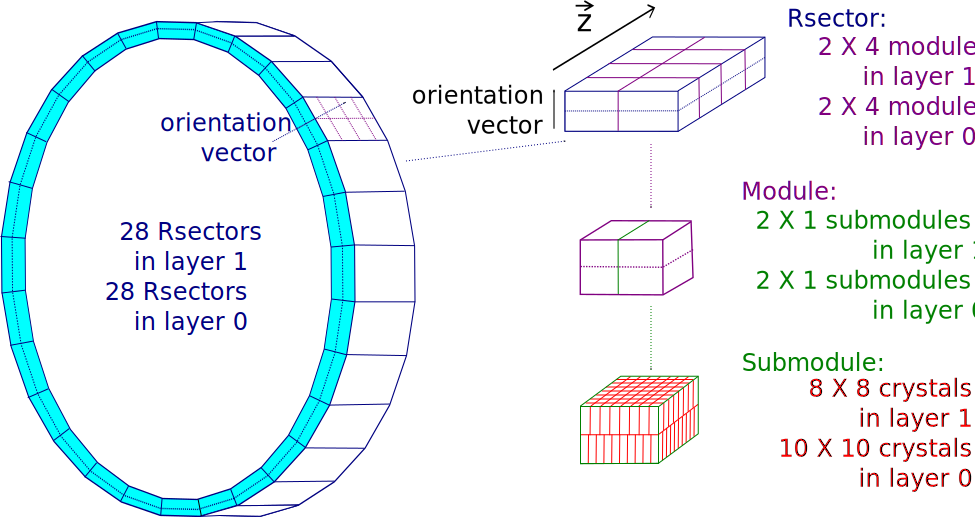
\includegraphics[width=0.8\columnwidth]{./figures/geo_decomposition.pdf}
  \caption{Illustration of the levels of decomposition of the PET scanner geometry, for a two-layer system.}
  \label{fig_scanner_decomposition}
\end{figure}

CASToR conventions about scanner elements indexation and orientations are illustrated in Figures~\ref{fig_scanner_axial_orientation} and~\ref{fig_scanner_description}. 
The elements numbering starts at zero.
The origin of the left-handed Cartesian coordinate system $(\mathbf{x,y,z})$ is centered axially and transversally on the scanner. 
By default, CASToR will position the center of the first rsector directly above the scanner isocenter, then arrange the following rsectors by spanning them
transversally over 360 degrees in the clockwise direction (as viewed from the front of the gantry) around the isocenter (see Figure~\ref{fig_scanner_description-a}).
The angular position of the first rsector relative to the ${\mathbf y}$ axis ($\theta_0$, $0\degree$ by default) and the angular span ($\Delta_{\theta}$, $360\degree$
span by default) are customizable (see Figure~\ref{fig_rsector}). 
For a system of $N$ rsectors, the angular position $\theta_i$ relative to the ${\mathbf y}$ axis of rsector $i$ is then given by
\begin{equation}
  \theta_i = i \times \frac{\Delta_{\theta}}{N} + \theta_0.
  \label{eq_rstorID}
\end{equation}

\begin{figure}
  \centerline{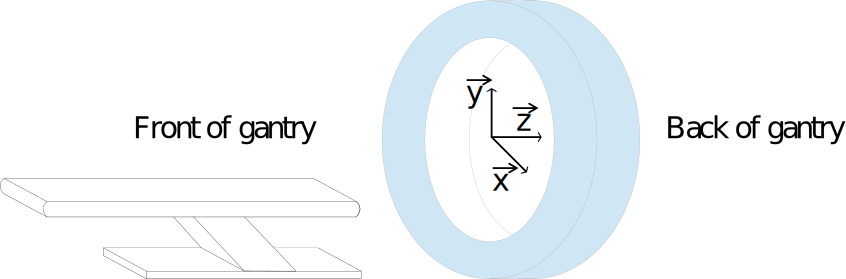
\includegraphics[width=0.6\columnwidth]{./figures/scanner_iso.pdf}}
  \caption{Left-handed Cartesian coordinate system $(\mathbf{x,y,z})$.}
  \label{fig_scanner_axial_orientation}
\end{figure}

\begin{figure}
  \centerline
  {
    \subfigure[Transverse indexation]{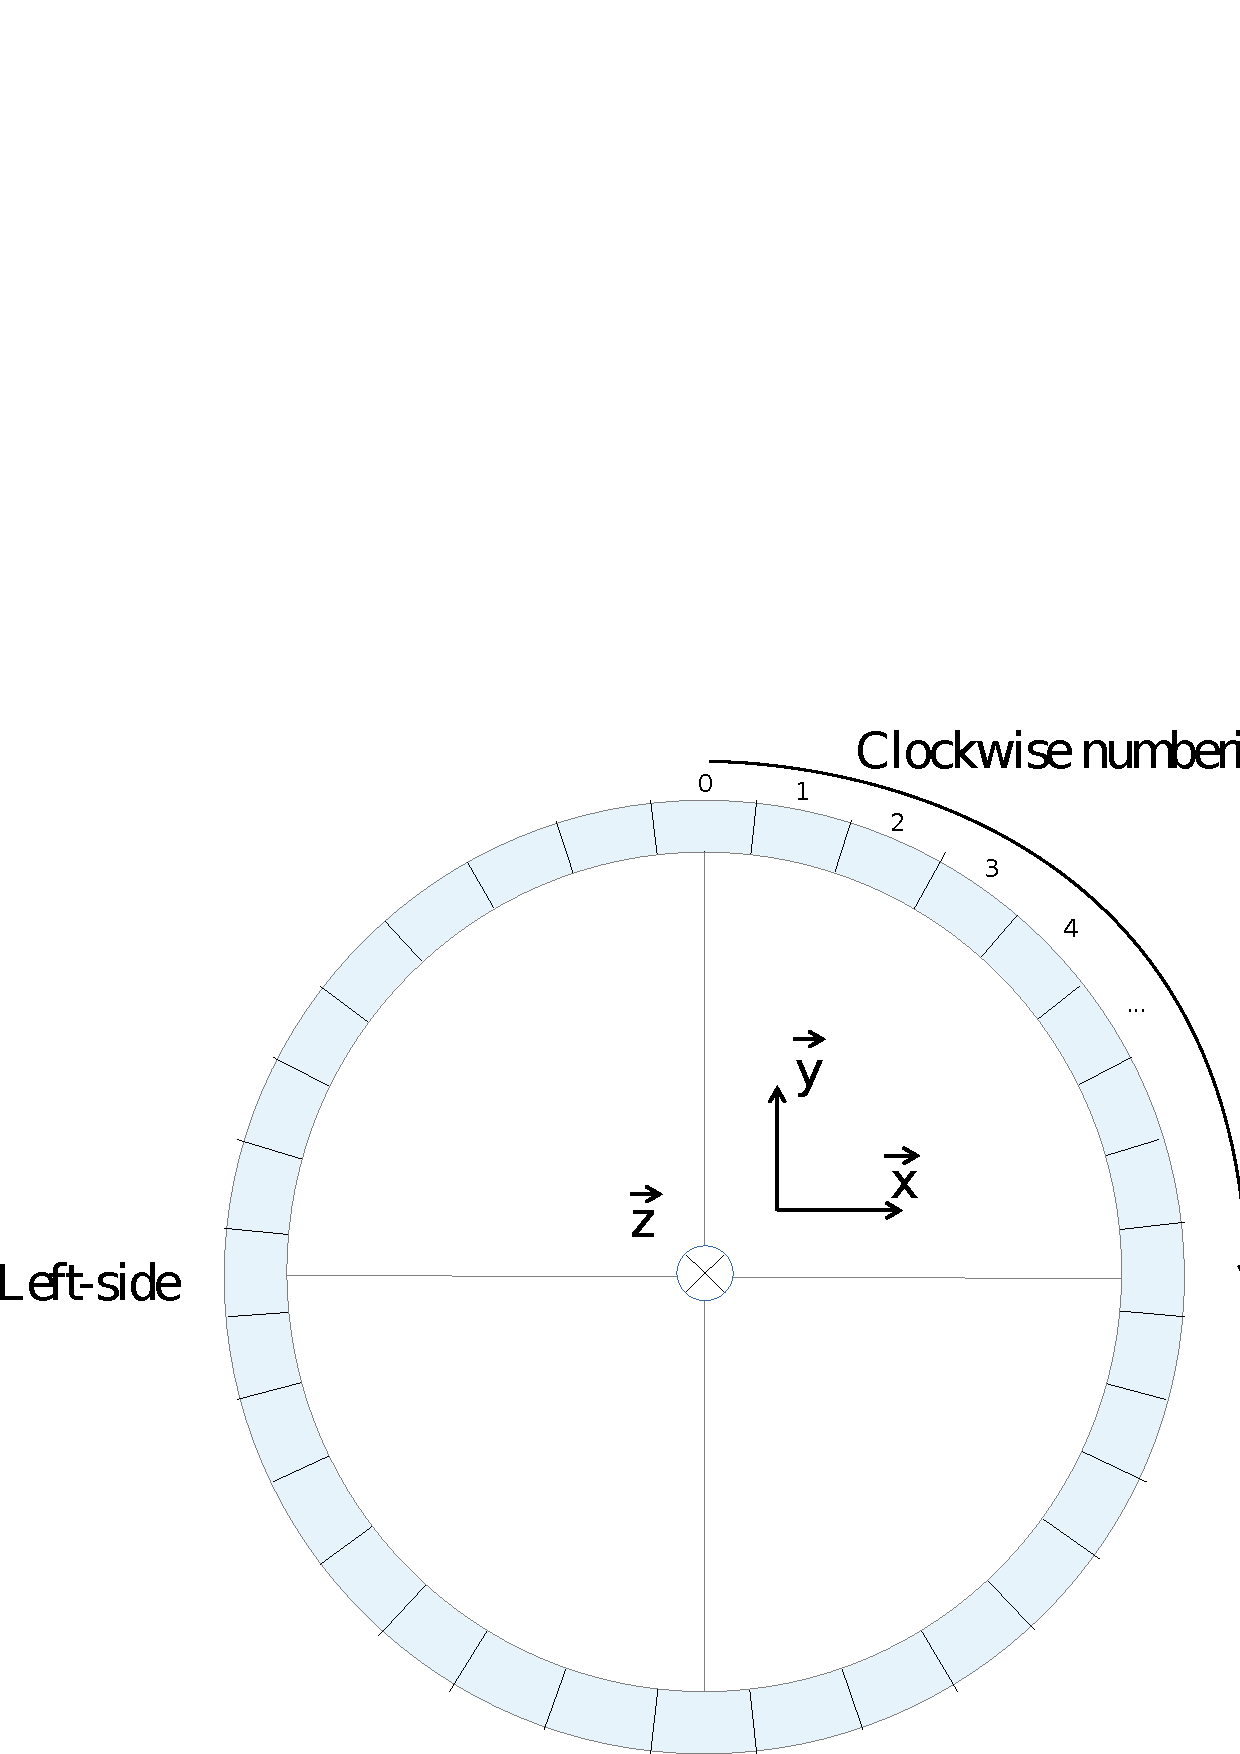
\includegraphics[width=0.6\columnwidth]{./figures/scanner_trans.pdf}
    \label{fig_scanner_description-a}}
    \subfigure[Axial indexation]{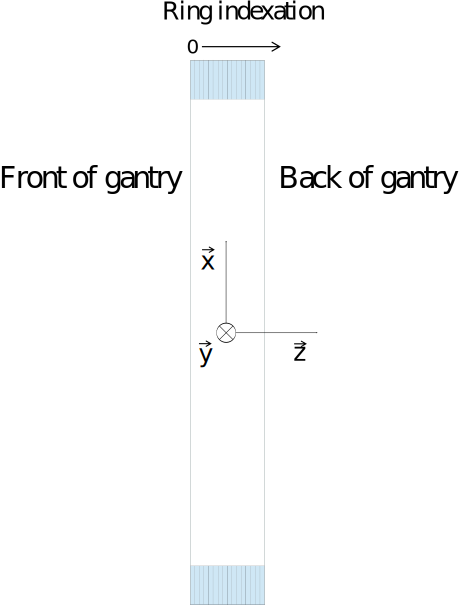
\includegraphics[width=0.3\columnwidth]{./figures/scanner_axial.pdf}\linebreak
    \label{fig_scanner_description-b}}
  }
  \caption
  {
    Transverse and axial indexations for PET scanner elements. 
    Numbering starts at zero. The orientation unit vector of each rsector is also displayed; its axial coordinate is null.
   (a) View from the front.
   (b) View from the bottom.
  }
  \label{fig_scanner_description}
\end{figure}

\begin{figure}
  \centerline{\includegraphics[width=0.8\columnwidth]{./figures/rsectors.pdf}}
  \caption
  {
    Angular spanning for a PET scanner consisting of 12 rsectors. Left: $\theta_0=0\degree$, $\Delta_{\theta}=360\degree$.
    Right: $\theta_0=45\degree$, $\Delta_{\theta}=180\degree$.
  }
  \label{fig_rsector}
\end{figure}

\paragraph{Crystal indexation} 
A unique identification number is assigned to each crystal of the PET scanner. 
All the events in the data file will be identified by these crystal numbers.
Crystals are first ordered transversally along a crystal ring, following a clockwise direction, and then axially across the crystal rings, from the front to
the back of the gantry (see Figure~\ref{fig_scanner_description}). 
The first crystal is located in the first rsector and, when  $\theta_0=0\degree$, possess the smallest value on the $\mathbf x$ axis.
If the scanner contains several layers, all the crystals of the first layers are indexed before switching to those of the next layer. 
For example, for a scanner containing two layers, the index of the first crystal of the second layer will be equal to the total number of crystals in the first layer.
Equation~\ref{eq_crystalID} provides the absolute crystal indexation $idCrystal$ for an one-layer system according to the variables below:

\begin{itemize}
  \item $nbRsectors$: number of \textbf{transaxial} rsectors
  \item $nbAxialRsectors$: \textbf{As of CASToR v1.2, a number of axial rsectors can also be provided (in effect, the rsector "ring" will be axially duplicated). This has been implemented for a better compatibility with the GATE Monte-Carlo simulation tools.}
  \item $nbAxialModules$ / $nbTransaxialModules$: number of axial/transaxial modules in a rsector
  \item $nbAxialSubmodules$ / $nbTransaxialSubodules$: number of axial/transaxial submodules in a module
  \item $nbAxialCrystals$ / $nbTransaxialCrystals$: number of axial/transaxial crystals in a submodule
  \item $idRsector$: rsector id
  \item $idAxialModule$ / $idTransaxialModule$: axial/transaxial module id in a rsector
  \item $idAxialSubmodule$ / $idTransaxialSubmodule$: axial/transaxial submodule id in a module
  \item $idAxialCrystal$ / $idTransaxialCrystal$: axial/transaxial crystal id in a submodule
\end{itemize}

\begin{equation}
\begin{aligned}
idCrystal = & idRing \times nbCrytalsPerRing \\
                 & + idTransaxialCrystal \\
                 & + idTransaxialSubmodule \times nbTransaxialCrystals \\
                 & + idTransaxialModule \times nbTransaxialSubmodules \times nbTransaxialCrystals\\
                & + idRsector \times nbTransaxialModules \times nbTransaxialSubmodules\\
                &  \times nbTransaxialCrystals,
\end{aligned}
\label{eq_crystalID}
\end{equation}
where the total number of crystals in a ring, $nbCrytalsPerRing$, is  given by
\begin{equation}
\begin{aligned}
nbCrytalsPerRing = & nbRsectors \times nbTransaxialModules \\
                            & \times nbTransaxialSubodules \times nbTransaxialCrystals
\end{aligned}
\label{eq_nCrytalsPerRing}
\end{equation}
and the ring index $idRing$ is given by
\begin{equation}
\begin{aligned}
idRing = & idAxialCrystal + idAxialSubmodules \times  nbAxialCrystals \\
              &+ idAxialModule \times nbAxialSubmodules \times nbAxialCrystals \\
              &+ idAxialRsector \times nbAxialModules \times nbAxialSubmodules \times nbAxialCrystals \\
\end{aligned}
\label{eq_idRing}
\end{equation}

\paragraph{Geom file structure}
The name of the .geom file should correspond to the scanner name, followed by the file extension geom.
The file shall be located in the scanner repository directory '\$\{CASTOR\_CONFIG\}/scanner',
where examples of .geom files for various PET scanner systems can be found.
The description of each mandatory and optional field in the .geom file is provided below. 
The fields are case sensitive. The separator (between the field and the value) is the colon sign ":".

\paragraph{Mandatory fields}  \
\\
\begin{itemize}
  \item \textbf{modality}: PET.
  \item \textbf{scanner name}: no restriction. Scanner names are usually referenced using the following template: 
        \texttt{Modality\_Manufacturer\_Model}, ({\it e.g.}: \texttt{PET\_Siemens\_mMR}).
  \item \textbf{description}: any string containing additional information about the scanner.
  \item \textbf{number of elements}: total number of crystals.
  \item \textbf{number of layers}: number of layers.
  \item \textbf{voxels number transaxial}: default number of voxels in the ${\mathbf x}$ and ${\mathbf y}$ directions for the reconstructed images
        (only used if the image matrix dimensions are not provided by the user in the command-line options (\textit{-dim})).
  \item \textbf{voxels number axial}: default number of voxels in the ${\mathbf z}$ direction for the reconstructed images (only used if the image
        matrix dimensions are not provided by the user in the command-line options (\textit{-dim})).
  \item \textbf{field of view transaxial}: default reconstructed transverse FOV in mm (only used if the FOV or voxel dimensions are not provided by
        the user in the command-line options (\textit{-fov} or \textit{-vox})).
  \item \textbf{field of view axial}: default reconstructed axial FOV in mm (only used if the FOV or voxel dimensions are not provided by the user
        in the command-line options (\textit{-fov} or \textit{-vox})).
\end{itemize}
 
The following variables depend on the number of  layers. 
In the event that the scanner contains several layers, each variable must list the values corresponding to each layer, separated by commas ({\it e.g.}:
\texttt{field: val\_layer1, val\_layer2}):

\begin{itemize}
  \item \textbf{scanner radius}: for each layer, radial distance in mm between the scanner isocenter and the front face of the rsectors (see
        Figure~\ref{fig_scanner_fields-a}).
  \item \textbf{number of rsectors}: for each layer, number of rotational (transaxial) sectors.
  \item \textbf{number of crystals transaxial}: for each layer, number of transverse crystals within a submodule.
  \item \textbf{number of crystals axial}: for each layer, number of axial crystals within a submodule.
  \item \textbf{crystals size depth}: for each layer, depth size in mm of the crystal along the orientation vector.
\end{itemize}

\paragraph{Optional fields} \
\\
The following optional variables also depend on the number of layers.

\begin{itemize}
  \item \textbf{crystals size trans}: for each layer, transverse size in mm of the crystal.
  \item \textbf{crystals size axial}: for each layer, axial size in mm of the crystal.
  \item \textbf{rsectors first angle}: for each layer, transaxial angular position in degree of the center of the first rsector (default is $0\degree$,
        see Figure~\ref{fig_rsector}).
  \item \textbf{rsectors angular span}: for each layer, the transverse angular span in degree of the rsectors  (default is $360\degree$, see
        Figure~\ref{fig_rsector}).        
  \item \textbf{number of rsectors axial}: As of CASToR v1.2, a number of axial rsectors (for each layer) can also be provided (default is 1).
  \item \textbf{rsector gap axial}:  As of CASToR v1.2, for each layer, axial gap in mm between two consecutive axial rsectors (default is 0.0 mm).
  \item \textbf{number of modules transaxial}: for each layer, number of transverse modules within a rsector (default is 1).
  \item \textbf{number of modules axial}: for each layer, number of axial modules within a rsector (default is 1).
  \item \textbf{module gap transaxial}: for each layer, transverse gap in mm between two consecutive modules within a rsector (default is 0.0 mm).
  \item \textbf{module gap axial}: for each layer, axial gap in mm between two consecutive modules within a rsector (default is 0.0 mm).
  \item \textbf{number of submodules transaxial}: for each layer, number of transverse submodules within a module (default is 1).
  \item \textbf{number of submodules axial}: for each layer, number of axial submodules within a module (default is 1).
  \item \textbf{submodule gap transaxial}: for each layer, transverse gap in mm between two consecutive submodules within a module (default is 0.0 mm).
  \item \textbf{submodule gap axial}: for each layer, axial gap in mm between two consecutive submodules within a module (default is 0.0 mm).
  \item \textbf{crystal gap transaxial}: for each layer, transverse gap in mm between two consecutive crystals within a submodule (default is 0.0 mm).
  \item \textbf{crystal gap axial}: for each layer, axial gap in mm between two consecutive crystals within a submodule (default is 0.0 mm).
  \item \textbf{mean depth of interaction}: for each layer, from the crystal front surface, mean depth of interaction in mm along the orientation vector
        (default is crystal depth size divided by 2).
\end{itemize}

The following optional variables do not depend on the number of layers.
\begin{itemize}
  \item \textbf{min angle difference}: minimum transverse angle difference in degree between two crystals to define a valid line of response.
        This parameter is principally used for the list-mode sensitivity image generation, in order to model any hardware restriction on the lines of
        response (default is $0\degree$,  see Figure~\ref{fig_scanner_fields-a}).
  \item \textbf{rsectors nbZShift}: number of distinct axial shift values for the rsector, similar  to the GATE~\cite{GATE} \textit{Zshift} definition
        (default is 0, see Figure~\ref{fig_scanner_fields-b}). 
  \item \textbf{rsectors ZShift}: axial shift values in mm, separated by commas. The number of values must be equal to the value provided in
        \textbf{rsectors ZShift}. The axial shift value for rsector $i$ is then given by $ZShift[i \pmod{nbZShift}]$. 
\end{itemize}
\begin{figure} [h!]
  \centerline
  {
    \subfigure[]
    {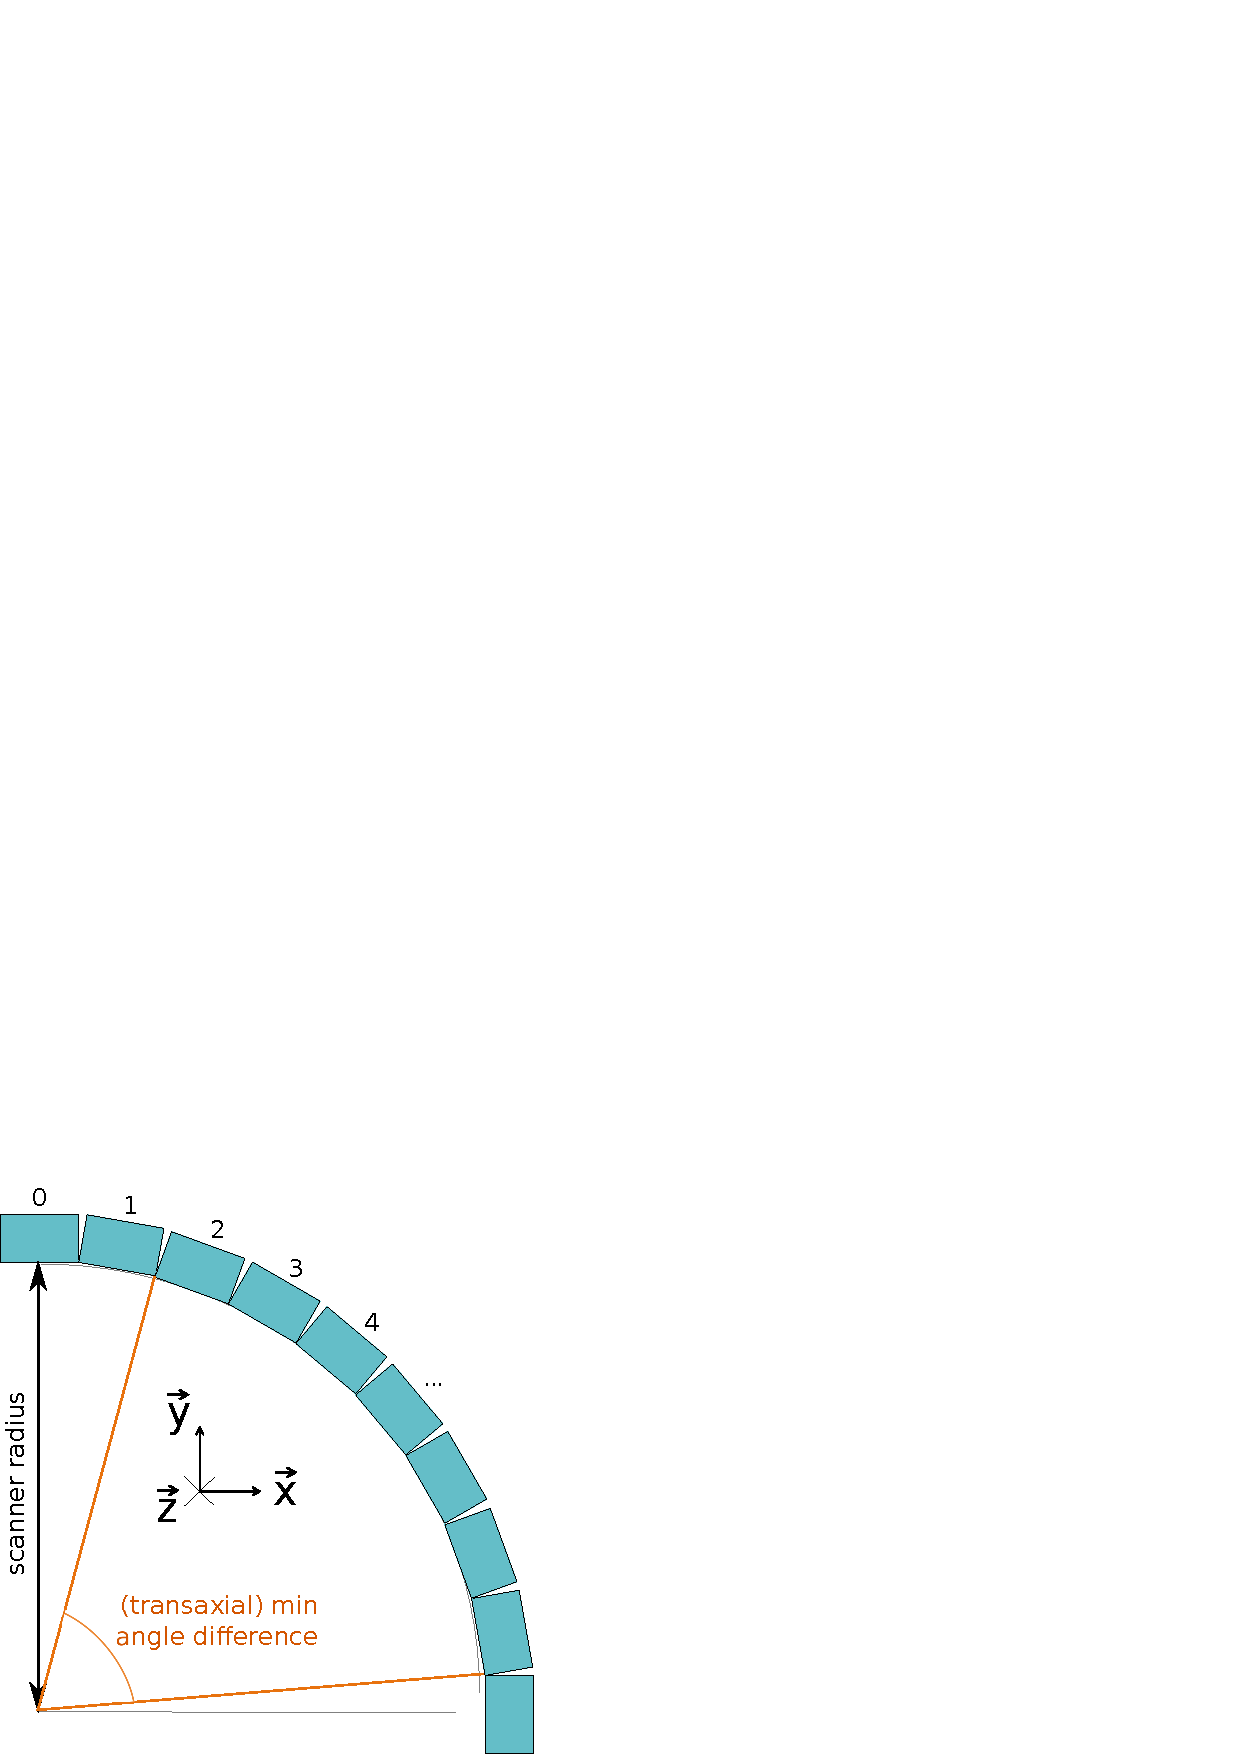
\includegraphics[width=0.50\columnwidth]{./figures/scanner_variable.pdf}
    \label{fig_scanner_fields-a}}\hspace{0.1\textwidth}
    \subfigure[]
    {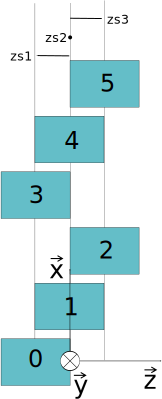
\includegraphics[width=0.20\columnwidth]{./figures/scanner_zshifts.pdf}
    \label{fig_scanner_fields-b}}
  }
  \caption
  {
    Illustration of several transverse (a) and axial (b) geometric variables related to the PET scanner configuration files. \\
    (a)\textbf{\textit{scanner radius}} is defined as the radial distance between the scanner isocenter and the front face of the rsector. 
    The \textbf{\textit{min angle difference}} represents the required minimal angular difference between two detectors to generate a line of response. \\
    (b) System with 3 different axial shifts $zs1, zs2, zs3$ (\textbf{\textit{rsectors nbZShift}} = 3 ; \textbf{\textit{rsectors ZShift}} = -10,0,+10 mm).
  }
  \label{fig_scanner_fields}
\end{figure}

The decomposition of the scanner geometry used in the .geom files should be sufficient to model the geometry of most known PET scanners. 
This is also the most user-friendly method to integrate a scanner as the reconstruction algorithm will generate itself the LUT. 
The user still has to perform the conversion from the original data indexation to the CASToR indexation, by applying Equation~\ref{eq_crystalID}. 
The \textit{castor-datafileConversionEx} script could be used in order to facilitate this operation (see section \ref{ss_utilities_conversion}).
Another way to integrate a PET scanner is by directly providing a LUT integrating the Cartesian coordinates and the orientation unit vector of all
the scanner detection elements, as described in section~\ref{sss_scanner_integration_PET_uLUT}.

%---------------------------------------------------------------------------------------------------------------------------------------------------------------
\subsubsection{Scanner integration using a pre-computed LUT file (.lut)}
\label{sss_scanner_integration_PET_uLUT}

This method is advised for scanners with unconventional design and for users who would like to generate a LUT with their own crystal indexation. 
The scanner LUT is composed of two files: an ASCII header file (with the .hscan file extension) containing metadata about the scanner specifications and
a binary data file (with the .lut file extension) containing the LUT. 
Both files must have the same basename, given by the scanner name, and be located in the scanner repository directory '\$\{CASTOR\_CONFIG\}/scanner'.

\paragraph{Binary LUT file}
The binary data in the .lut file must contain a number of {\it words} equal to the number of elementary detection units (typically, crystals for PET scanners). 
The content of each word is described in Table~\ref{table_lut}. 
It defines the coordinates and the orientation of the elementary detection unit along its depth in the left-handed Cartesian coordinate system described in
Figure~\ref{fig_scanner_axial_orientation}. 

It is possible to group the elementary detection units into \textit{layers}: all elementary detection units within a given layer have the same depth size.
If the system consists of only one layer, then all the elementary detection units have the same depth size.
It is also possible to group the elementary detection units within a layer into \textit{rings}.
The number of elementary detection units and the number of rings can vary between layers,
but for a given layer, the number of elementary detection units per ring is constant.  
For list-mode reconstruction, any restriction on the co-polar aperture can be set using the \textit{maximum axial difference mm} variable in the datafile header (see section \ref{ss_input_PET}). This value defines a global (for all layers) maximum axial difference in mm between two crystals in a lor.

For a system consisting of {\tt NLayer} layers and {\tt NRing[iLayer]} rings and {\tt NDet[iLayer]} elementary detection units per layer {\tt iLayer}, 
the writing of the elementary detection unit words in the LUT file  shall satisfy the following order: 
\begin{lstlisting}[caption=,numbers=none]
for(iLayer=0;iLayer<NLayer;iLayer++) 
 for(iRing=0;iRing<NRing[iLayer];iLayer++) 
  for(iDet=0;iDet<NDet[iLayer]/NRing[iLayer];iDet++) {
   fwrite(&Posx[iLayer][iRing][iDet],sizeof(FLTNBLUT),1,fPtr);
   fwrite(&Posy[iLayer][iRing][iDet],sizeof(FLTNBLUT),1,fPtr);
   fwrite(&Posz[iLayer][iRing][iDet],sizeof(FLTNBLUT),1,fPtr);
   fwrite(&OrVx[iLayer][iRing][iDet],sizeof(FLTNBLUT),1,fPtr);
   fwrite(&OrVy[iLayer][iRing][iDet],sizeof(FLTNBLUT),1,fPtr);
   fwrite(&OrVz[iLayer][iRing][iDet],sizeof(FLTNBLUT),1,fPtr);
}
\end{lstlisting}
%\begin{multline*}
%\mathrm{for}(i_{\mathrm{layer}}=0;i_{\mathrm{layer}}<N_{\mathrm{layer}};i_{\mathrm{layer}}++) \\
% \mathrm{for}(i_{\mathrm{ring}}=0;i_{\mathrm{ring}}<N_{\mathrm{ring}}[i_{\mathrm{layer}}];i_{\mathrm{layer}}++)  \\
%   \mathrm{for}(i_{\mathrm{crystal}}=0;i_{\mathrm{crystal}}<N_{\mathrm{crystal}}[i_{\mathrm{layer}}][i_{\mathrm{ring}}];i_{\mathrm{crystal}}++) \\
%      \mathrm{fwrite}(posX[i_{\mathrm{layer}}][i_{\mathrm{ring}}][i_{\mathrm{crystal}}]
%\end{multline*}

\begin{table} [h!]
  \small
  \caption
  {
    The content of one word, corresponding to one elementary detection unit, in the binary LUT file. 
    Distances are given in mm. 
    The default data type is single-precision floating-point.
    The data type can be changed by editing the variable 'FLTNBLUT' in the 'gVariables.hh' file (see Section~\ref{ss_install_precision}).
    The orientation unit vector shall satisfy $OrVx^2 + OrVy^2 + OrVz^2=1$.
  }
  \label{table_lut}
  \begin{center}
  \begin{tabular}{|c|c|}
  \hline
  \textit{\textbf{Tag}} & \textit{\textbf{Description}} \\
  \hline
  Posx & Position of the center of the elementary detection unit on the X-axis \\ 
  \hline
  Posy & Position of the center of the elementary detection unit on the Y-axis \\ 
  \hline
  Posz & Position of the center of the elementary detection unit on the Z-axis\\ 
  \hline
  OrVx & Orientation unit vector of the elementary detection unit on the X-axis \\ 
  \hline
  OrVy & Orientation unit vector of the elementary detection unit on the Y-axis \\ 
  \hline
  OrVz & Orientation unit vector of the elementary detection unit on the Z-axis \\ 
  \hline
  \end{tabular}
  \end{center}
\end{table}

\paragraph{Header LUT file}
The content of the ASCII LUT header file is described below. It includes mandatory and optional fields. The keywords are case sensitive.
The separator (between the field and the value) is the colon sign ":".
\paragraph{Mandatory fields}
\begin{itemize}
  \item \textbf{modality}: PET.
  \item \textbf{scanner name}: no restriction. Scanner names are usually referenced using the following template: 
       \texttt{Modality\_Manufacturer\_Model}, ({\it e.g.}: \texttt{PET\_Siemens\_mMR}).
  \item \textbf{description}: any string containing additional information about the scanner.
  \item \textbf{number of elements}: total number of elementary detection units (typically, crystals in PET).
  \item \textbf{number of layers}: number of layers.
  \item \textbf{voxels number transaxial}: default number of voxels in the ${\mathbf x}$ and ${\mathbf y}$ directions for the reconstructed
        images (only used if the image matrix dimensions are not provided by the user in the command-line options (\textit{-dim})).
  \item \textbf{voxels number axial}: default number of voxels in the ${\mathbf z}$ direction for the reconstructed images (only used  if the
        image matrix dimensions are not provided by the user in the command-line options (\textit{-dim})).
  \item \textbf{field of view transaxial}: default reconstructed transverse FOV in mm (only used if the FOV or voxel dimensions are not provided
        by the user in the command-line options (\textit{-fov} or \textit{-vox})).
  \item \textbf{field of view axial}: default reconstructed axial FOV in mm (only used  if the FOV or voxel dimensions are not provided by the
        user in the command-line options (\textit{-fov} or \textit{-vox})).
\end{itemize}
The following variables depend on the number of layers. 
In the event that the scanner contains several layers, each variable must list the values corresponding to each layer, separated by commas
({\it e.g.}: \texttt{field: val\_layer1, val\_layer2}):
\begin{itemize}
  \item \textbf{number of crystals in layer}: for each layer, number of elementary detection units (typically, crystals in PET).
  \item \textbf{crystals size depth}: for each layer, depth size in mm of the elementary detection units along the orientation vector (typically,
        crystals in PET).
  %\item \textbf{crystals size trans}: for each layer, transverse size in mm of the elementary detection units (typically, crystals in PET).
  %\item \textbf{crystals size axial}: for each layer, axial size in mm of the elementary detection units (typically, crystals in PET).
\end{itemize}

\paragraph{Optional fields}
\begin{itemize}
  \item \textbf{mean depth of interaction}: for each layer, from the elementary detection unit front surface, mean depth of interaction in mm along
        the orientation vector  (default is elementary detection unit depth size divided by 2).
  \item \textbf{min angle difference}: minimum transverse angle difference in degree between two crystals to define a valid line of response.
        This parameter is principally used for the list-mode sensitivity image generation, in order to model any hardware restriction on the lines
        of response (default is $0\degree$,  see Figure~\ref{fig_scanner_fields-a}). There is a unique value for all layers. 
        
\end{itemize}

%---------------------------------------------------------------------------------------------------------------------------------------------------------------
%---------------------------------------------------------------------------------------------------------------------------------------------------------------
\newpage
\subsection{SPECT systems using parallel/convergent collimators}
\label{ss_scanner_integration_SPECT_conv}

The most important part of SPECT reconstruction consists in the modelling of the collimator which will affect the solid angle providing the probability
of a photon originating from the scanned object to reach the gamma camera. Due to the numerous types and geometries of SPECT parallel and convergent
collimators, CASToR does not rely on the full modeling of the collimator in the projector. Instead, the collimator is characterized by a polynomial
equation whose coefficients are defined in the SPECT gamma camera configuration file. The order and parameters of the polynomial equations allow to
specify the collimator type and features. The couple of SPECT data indices, defined as a projection angle associated to a crystal/pixel pair, are used
to compute a focal point. Cartesian positions of this focal point and the crystal/pixel of the gamma camera allows to outline a projection ray/volume.

Although CASToR uses polynomial equations by default to characterize the different types of collimator, one can implement his own model in the SPECT
geometry class to estimate the focal point of a gamma camera pixel/projection angle couple, or even model the entire geometry of the collimator in a
projector class.

%---------------------------------------------------------------------------------------------------------------------------------------------------------------
\subsubsection{Scanner integration using a generic file (.geom)}
\label{sss_SPECT_conv_geom}

The .geom ASCII file for SPECT scanners contains information about the structural design of the SPECT gamma camera head(s), and the focal model and
parameters which characterize the collimator.

The description of each mandatory and optional field in the geom file is provided below. The keywords are case sensitive.
The separator (between the field and the value) is the colon sign ":".\\

\paragraph{General fields}:
\begin{itemize}
  \item \textbf{modality}: \texttt{SPECT\_CONVERGENT}
  \item \textbf{scanner name}: no restrictions, but it is adviced to follow the following template:\\
        \texttt{Modality\_Constructor\_Model} (\textit{e.g.} \texttt{SPECT\_Siemens\_INTEVO}).
  \item \textbf{number of detector heads}: total number of heads in the SPECT system
  \item \textbf{trans number of pixels}: total number of transaxial pixels (crystals) in the gamma camera head(s) (1 for monolythic cameras).
  \item \textbf{trans pixel size}: Transaxial size of each pixel/crystal in mm
  \item \textbf{trans gap size}: Transaxial gap between pixels/crystals in mm
  \item \textbf{axial number of pixels}: total number of axial pixels (crystals) in the gamma camera head(s) (1 for monolythic cameras).
  \item \textbf{axial pixel size}: Axial size of each pixel/crystal in mm
  \item \textbf{axial gap size}: Axial gap between pixels/crystals in mm
  \item \textbf{detector depth}: Crystal depth (mm). This parameter is currently not used in CASToR reconstruction, but is included here for future
        developements. The following variables depend on the number of detector heads. If the SPECT system contains several heads, each variable
        must list the values corresponding to each head, separated by commas.
  \item \textbf{scanner radius}: default global distance in mm between the scanner's center of rotation (COR) and the head's collimator. If this
        distance is dependent on the projection angle, this information must be provided in the datafile header and will overwrite this value.
\end{itemize}

The following variables are related to the collimator configuration. If the SPECT system contains several heads, the set of parameters specific to
each head must be provided and preceded of the head they belong to (\textit{head1}, \textit{head2}, etc):

\begin{itemize}
  \item \textbf{trans focal model}: string corresponding to the transaxial focal model. Must be \textit{constant}, \textit{polynomial},
        \textit{slanthole}, or \textit{custom}
  \item \textbf{trans number of coef model}: Number of parameters for the transaxial model. Must be 1,2 or 3 for \textit{polynomial} (see eq. \ref{eq_sss_SPECT_colli_pol0} below),
        1 for \textit{slanthole} (see eq. \ref{eq_sss_SPECT_colli_slant}), or any number for \textit{custom}. This parameter is discarded for the \textit{constant} model.
  \item \textbf{trans parameters}: A number of parameters corresponding to the previous field, separated by commas. For the polynomial model, coefficients must be given in ascending degree order (c,b,a, as defined in eq. \ref{eq_sss_SPECT_colli_pol0} below)).
  \item \textbf{axial focal model}: string corresponding to the axial focal model. Must be \textit{constant}, \textit{polynomial},
        \textit{slanthole}, or \textit{custom}.
  \item \textbf{axial number of coef model}: Number of parameters for the transaxial model. Must be 1,2 or 3 for \textit{polynomial} (see eq. \ref{eq_sss_SPECT_colli_pol0} below),
        1 for \textit{slanthole}  (see eq. \ref{eq_sss_SPECT_colli_slant}), or any number for \textit{custom}. This parameter is discarded for the \textit{constant} model.
  \item \textbf{axial parameters}: A number of parameters corresponding to the previous field, separated by commas. For the polynomial model, coefficients must be given in ascending degree order (c,b,a, as defined in eq. \ref{eq_sss_SPECT_colli_pol0} below)).
\end{itemize}

%---------------------------------------------------------------------------------------------------------------------------------------------------------------
\subsubsection{Collimator focal model defined by the (.geom) file}
\label{sss_SPECT_conv_colli}

The current implementation of SPECT parallel and convergent collimators in CASToR relies on several models, which either apply to the
transaxial or axial directions. Different models could be selected for the transaxial/axial direction in order to model collimators such
as a fan-beam for example. These models are listed below:

\paragraph{constant:}

The \textit{constant} model (Fig. \ref{fig_SPECT_colli_constant}) defines a parallel hole collimator. It does not require any parameters as
the focal point axial/transaxial geometric position will be computed as the symetrical opposite to the SPECT pixel relatively to the axial/transaxial plane parallel to the detector surface and containing origin. A parallel collimator requires constant models for both axial/transaxial directions while a fan-beam collimator requires a constant model for one of these directions.

\begin{figure} [h]
  \centering
  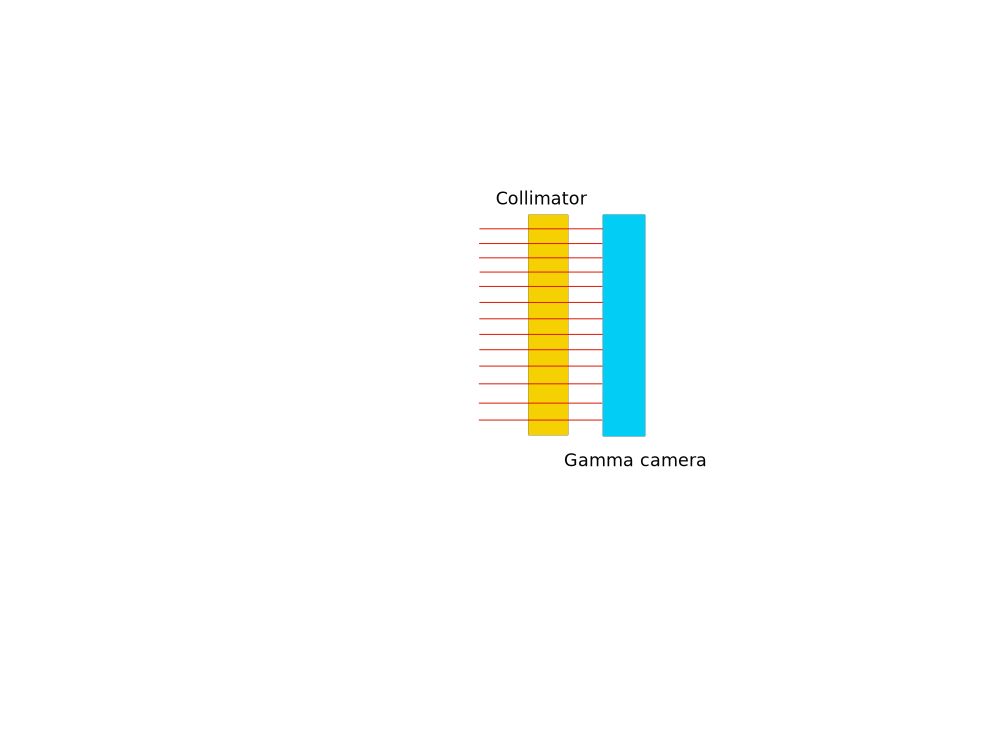
\includegraphics[width=0.23\columnwidth]{./figures/spect_colli_parallel.pdf}
  \caption{Constant model for SPECT collimator}
  \label{fig_SPECT_colli_constant}
\end{figure}

\paragraph{polynomial:}

The \textit{polynomial} model allows to characterize convergent and multi-convergent collimators using
polynomial equations of different order to compute the focal point(s). The polynomial expression is interpreted in mm (the default distance
unit used in CASToR). The axial/transaxial focal length corresponding to a SPECT pixel in the axial/transaxial plane is located on the optical axis (line orthogonal to and centered on the detector surface), and whose position is computed as:

\begin{equation}
\begin{aligned}
f(x) = ax^2 + b|x| + c
\end{aligned}
\label{eq_sss_SPECT_colli_pol0}
\end{equation}

where, x corresponds to the axial/transaxial distance between the SPECT pixel position, and its orthogonal projection on the optical axis (Fig. \ref{fig_SPECT_colli_polynomial}).

A polynomial function with one coefficient (degree 0) results in a mono-convergent (or mono-divergent if a negative coefficient is provided)
collimator on a specific direction, as each crystal of the gamma camera for a given projection angle will have a similar focal point (Fig.
\ref{fig_SPECT_colli_polynomial_1}) on that direction. A fan-beam collimator can be modeled as a collimator with a constant model on one of
the transaxial/axial direction, and a degree 0 polynomial model on the other direction. A mono-convergent cone-beam collimator corresponds
to a polynomial model for each direction.

A polynomial function with two or three coefficients (degree 1 or 2) results in a multi-convergent (or multi-divergent if a negative coefficient
is provided) collimator on a specific direction, as each crystal of the gamma camera for a given projection angle will have a different focal
point on that direction (Figs. \ref{fig_SPECT_colli_polynomial_2} and \ref{fig_SPECT_colli_polynomial_3}).


\begin{figure} [h]
  \centerline
  {
    \subfigure[Polynomial, degree 0]{
\includegraphics[width=0.30\columnwidth]{./figures/spect_colli_conebeam.pdf}
    \label{fig_SPECT_colli_polynomial_1}}
    \subfigure[Polynomial, degree 1]{
\includegraphics[width=0.34\columnwidth]{./figures/spect_colli_fanbeam.pdf}
    \label{fig_SPECT_colli_polynomial_2}}
    \subfigure[Polynomial, degree 2]{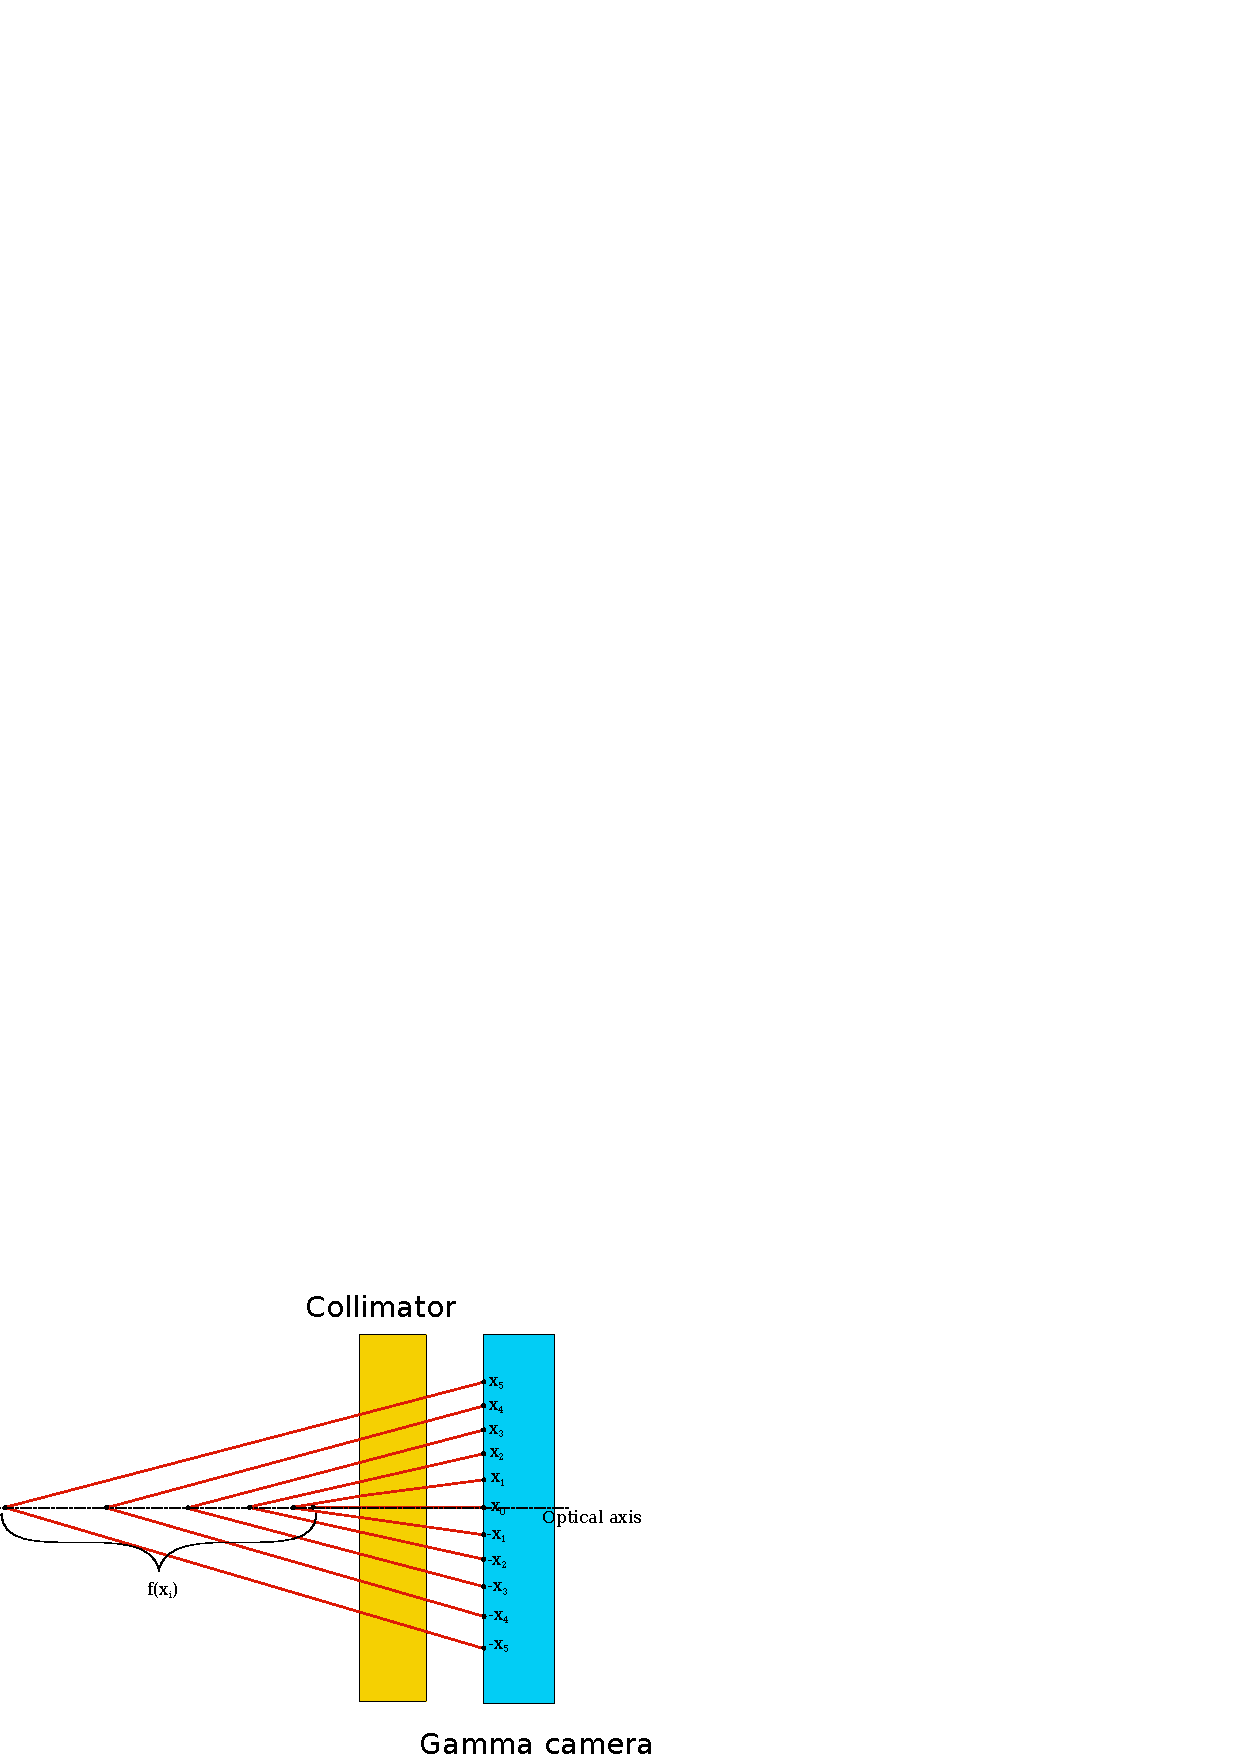
\includegraphics[width=0.45\columnwidth]{./figures/spect_colli_pln_deg2.pdf}\linebreak
    \label{fig_SPECT_colli_polynomial_3}}
  }
  \caption{Polynomial models for SPECT collimators using either one (a), two (b) or three (c) coefficients. $x_i$ represent the distances between each pixel i reference position and the optical axis (either in the axial or transaxial plane)}
  \label{fig_SPECT_colli_polynomial}
\end{figure}

\paragraph{slanthole:}

The \textit{slanthole} model (Fig. \ref{fig_SPECT_colli_slanthole}) allows to characterize slanthole collimators using polynomial equations
of degree 1 to compute the focal point(s). The slanthole model is a specific case of parallel hole collimators where all the collimator septas
are rotated according to a given angle. The focal position is computed as

\begin{equation}
\begin{aligned}
f(x) = ax
\end{aligned}
\label{eq_sss_SPECT_colli_slant}
\end{equation}

where, \textit{a} corresponds to the slanthole unique coefficient defining the angle $\alpha$ of the collimator, while \textit{sign(a)} defines the angle orientation. \textit{a} corresponds to $tan(\alpha)$. 

\begin{figure} [h!]
  \centering
  
\includegraphics[width=0.2\columnwidth]{./figures/spect_colli_slanthole.pdf}
  \caption{Slanthole models for SPECT slanthole collimators}
  \label{fig_SPECT_colli_slanthole}
\end{figure}

\paragraph{custom:}

The \textit{custom} model provides the opportunity for the user to implement his own collimator model characterized by his own equations
(such as hyperbolic or any other kind of equation). In the current CASToR version, the custom model must be implemented in the
\textit{iScannerSPECTConv::ComputeFocalPositions()} function in the \textit{src/scanner/iScannerSPECTConv.cc} file, in the conditionnal
statements related to the "custom" model, for both axial and transaxial focal position estimations. The current implementation of the
custom model returns an error by default.

%---------------------------------------------------------------------------------------------------------------------------------------------------------------
\subsubsection{Acquisition-specific geometry information}
\label{sss_SPECT_conv_acquisition_data}

The SPECT geometry will use several acquisition-specific information from the datafile header in order to generate the geometry (see
section \ref{ss_input_SPECT_conv} because more keywords can be used).
The keywords are case sensitive.
The separator (between the field and the value) is the colon sign ":".

\paragraph{Number of projections:}

The total number of projections (for all heads if the system contains more than one gamma camera) will be read from the datafile header.

\paragraph{Projection angles:}

The Cartesian positions of each pixel/crystal of the gamma camera and their corresponding focal points will be computed for each projection
angles. The projection angles must therefore be provided in the datafile header. If the SPECT system contains several heads, the angles for
the first head must be entered first, followed by the angles of the second head, etc.

\paragraph{Zoom:}

The zoom applied during the acquisition, for monolithic detectors. Along with the total size of the detector, it will be used to compute the effective
size of the detector in the transaxial and axial directions. Then the transaxial and axial sizes of the acquisition bins (see the next keyword) will
be deduced from this effective size of the detector (the rest of the detector will not acquire any counts).
This keyword is optional and its default value is 1.

\paragraph{Number of bins:}

The transaxial and axial number of bins must be provided in the datafile header. The pixel sizes will be computed from the number of bins and the gamma camera size. If this information is not provided (as for a pixellated detector),
the related fields from the SPECT configuration file (\textit{transaxial/axial number of pixels}) will be used instead. Pixels contained in each axial row must be subsequently indexed, starting from the pixels with the smallest x and z Cartesian positions (considering the head is located directly above the center of rotation), as presented in Fig. \ref{fig_pixel_indexation_spect}. 

\begin{figure} [h!]
  \centering
  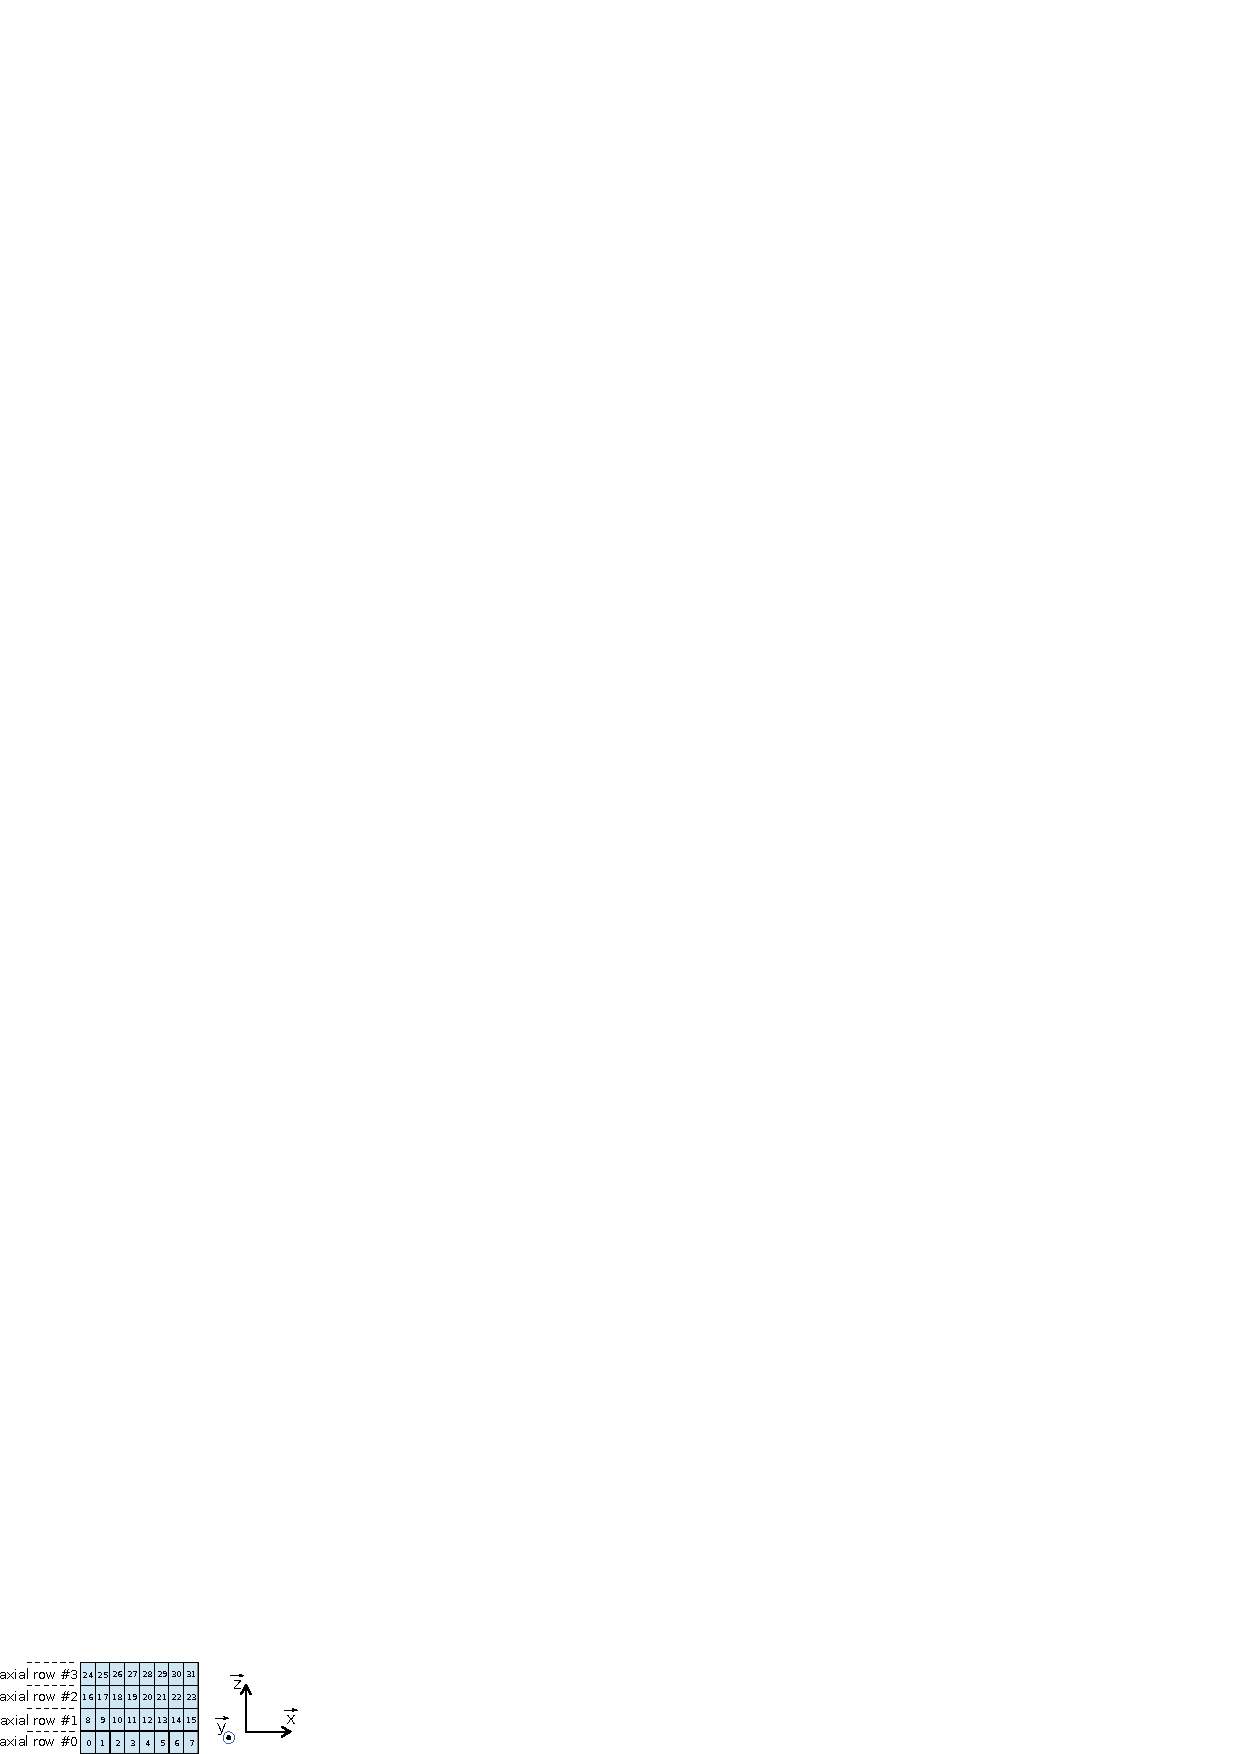
\includegraphics[width=0.4\columnwidth]{./figures/indexation_SPECT.pdf}
  \caption{Pixel indexation in a SPECT gamma camera with 4 axial rows of 8 transaxial pixels.}
  \label{fig_pixel_indexation_spect}
\end{figure}


\paragraph{(Global) Distance camera surface to COR:}

The distance between the center of rotation and the detector surface will be read from the datafile before computing the focal points and crystal's
geometric Cartesian locations. If this distance depends on the projection angle, the distance corresponding to each projection angle must be
provided after the field \textbf{\textit{Distance camera surface to COR}} (all values separated by commas). If this distance is similar for each
projection angle, one value must be provided by the field \textbf{\textit{Global distance camera surface to COR}}.

If none of these are provided in the datafile, the values given from the SPECT configuration file (\textbf{\textit{scanner radius}} tag)
will be used instead.

%---------------------------------------------------------------------------------------------------------------------------------------------------------------
\subsubsection{Scanner integration using a pre-computed LUT file (.lut)}
\label{sss_scanner_integration_SPECT_uLUT}

This part is not implemented for SPECT.


%---------------------------------------------------------------------------------------------------------------------------------------------------------------
%---------------------------------------------------------------------------------------------------------------------------------------------------------------
\subsection{CT systems}
\label{ss_scanner_integration_CT}

%---------------------------------------------------------------------------------------------------------------------------------------------------------------
\subsubsection{Scanner integration using a generic geometry file (.geom)}
\label{sss_scanner_integration_CT_geom}

The .geom file is an ASCII file containing information about the structural design of a flat panel CT.

\paragraph{Crystal indexation} 
A unique identification number is assigned to each detection pixel of the CT detector.
All the events in the data file will be identified by an angular view index as well as a pixel ID.
For the case of the detector being perpendicular to the X axis and positioned on its positive side, pixels are first ordered axially from the negative to the positive Z directions, and then ordered transaxially from the negative to the positive Y directions.

\paragraph{Geom file structure}
The name of the .geom file should correspond to the scanner name, followed by the file extension geom.
The file shall be located in the scanner repository directory '\$\{CASTOR\_CONFIG\}/scanner'.
The description of each mandatory and optional field in the .geom file is provided below. 
The fields are case sensitive. The separator (between the field and the value) is the colon sign ":".
Current assumptions:
\begin{itemize}
  \item The detector is a rectangular flat panel equally divided into pixels of detection.
  \item The source is supposed to be centered with respect to the detector both in transaxial and axial directions.
  \item The detector is supposed to be tangential to the scanner radius; no freedom angles.
  \item The distance between the center of rotation and the source is fixed in the scanner description.
  \item The distance between the center of rotation and the detector panel is fixed in the scanner description.
\end{itemize}

\paragraph{Mandatory fields}  \
\\
\begin{itemize}
  \item \textbf{modality}: CT
  \item \textbf{scanner name}: no restriction. Scanner names are usually referenced using the following template: 
        \texttt{Modality\_Manufacturer\_Model}, ({\it e.g.}: \texttt{CBCT\_VARIAN\_TRUEBEAM})
  \item \textbf{description}: any string containing additional information about the scanner
  \item \textbf{trans number of pixels}: the number of pixels along the transaxial direction
  \item \textbf{trans pixel size}: the size of the pixels along the transaxial direction, given in mm
  \item \textbf{trans gap size}: the size of the gaps between pixels along the transaxial direction, given in mm
  \item \textbf{axial number of pixels}: the number of pixels along the axial direction
  \item \textbf{axial pixel size}: the size of the pixels along the axial direction, given in mm
  \item \textbf{axial gap size}: the size of the gaps between pixels along the axial direction, given in mm
  \item \textbf{detector depth}: the depth of the pixels, given in mm
  \item \textbf{detector radius}: the distance between the center of rotation of the scanner and the surface of the detector, given in mm
  \item \textbf{source radius}: the distance between the center of rotation of the scanner and the source, given in mm
  \item \textbf{spot size width}: the width of the source that will be used for focal positions (the direction tangential to the scanner radius), given in mm
  \item \textbf{spot size height}: the height of the source that will be used for focal positions (the direction parallel to the scanner rotation axis), given in mm
\end{itemize}

%---------------------------------------------------------------------------------------------------------------------------------------------------------------
\subsubsection{Scanner integration using a pre-computed LUT file (.lut)}
\label{sss_scanner_integration_CT_uLUT}

This part is not yet implemented.

%---------------------------------------------------------------------------------------------------------------------------------------------------------------
%---------------------------------------------------------------------------------------------------------------------------------------------------------------
%---------------------------------------------------------------------------------------------------------------------------------------------------------------
%                I N P U T   D A T A F I L E
%---------------------------------------------------------------------------------------------------------------------------------------------------------------
%---------------------------------------------------------------------------------------------------------------------------------------------------------------
%---------------------------------------------------------------------------------------------------------------------------------------------------------------
\newpage
\section{CASToR input datafile format}
\label{s_input_files}

As explained in section~\ref{s_architecture}, CASToR uses an unified description for input data to be reconstructed. This section describes the format
of the datafile for the different data types (PET, SPECT, CT) and data mode (histogram, list-mode and normalization). Each datafile consists in two
separate files: an ascii header and a binary \textit{datafile}. The header contains all mandatory information about the acquisition, the system, the data
type, as well as information about the optional correction factors embeded into the datafile. The binary \textit{datafile} contains the raw data from the
acquisition (or the simulation), described by a series of \textit{events} gathering several mandatory and optional fields. These fields depend on the
modality and acquisition types.

There are no predefined file extension for CASTOR datafiles. The ascii header file is provided to the reconstruction program, and this header file
contains the name of the associated binary datafile. However, we commonly use the \textit{.cdh} and \textit{.cdf} extensions for header and binary
file respectively, standing for \textit{CASToR data header/file}.

%---------------------------------------------------------------------------------------------------------------------------------------------------------------
%---------------------------------------------------------------------------------------------------------------------------------------------------------------
\subsection{PET datafile format}
\label{ss_input_PET}

By PET data, we mean PET data linked to a PET geometry as described in section~\ref{ss_scanner_integration_PET}. In this context, some PET scanners
include intrinsic compression of the data channels, either axially (\textit{e.g.} span) or over the azimuthal angles (\textit{e.g.} mashing). Raw data
may have been also saved using compression factors. Note here that we do not talk about computer compression (\textit{e.g.} zip, rar or any proprietary
compression algorithm). To deal with this situation in a generic way (\textit{i.e.} without any manufacturer's specific methodology), CASToR uses
an optional field in the ascii header file specifying the maximum number of data channels contributing to a given event. If this number is
higher than 1, for each event in the binary datafile, the actual number of data channels contributing to this event is given, followed by the
list of all these data channels. This mechanism holds for any mode of data.

PET datafiles can contain histogram or list-mode data with associated corrections. An additional datafile mode can be used to describe the whole set of
operational data channels with their associated normalization factors. When performing a list-mode reconstruction, the normalization datafile can be
used to compute the sensitivity image. The loop will then be performed over the normalization \textit{events} (one per data channel) contained in the
normalization datafile, taking the normalization factors into account. If not provided, a loop over the scanner elements is performed, assuming a
uniform efficiency and no compression. For the sensitivity computation, an attenuation image containing attenuation coefficients (in cm$^{-1}$) can be
provided to correct for attenuation (providing the attenuation correction factors are also present in the datafile to be reconstructed). When using
a normalization datafile to compute this sensitivity image, the attenuation correction factors can also be embeded so that they are taken into
account during the computation (again providing the attenuation correction factors are also present in the datafile to be reconstructed). The normalization file is identical for data with and without TOF information.

%---------------------------------------------------------------------------------------------------------------------------------------------------------------
\subsubsection{ASCII header}

The content of the ascii header file is described below. It includes mandatory and optional fields. All keywords are case sensitive and the
separator (between the field and the value) is the colon sign ":".


\paragraph{Mandatory fields}
\begin{itemize}
  \item \textbf{Scanner name}: The name of the PET scanner (corresponding to a scanner in the \textit{config/scanner} folder, without
        the file extension)
  \item \textbf{Data filename}: The absolute or relative path to the binary datafile
  \item \textbf{Number of events}: The number of CASToR events in the binary datafile
  \item \textbf{Data mode}: Can be "list-mode", "histogram" or "normalization"
  \item \textbf{Data type}: PET
  \item \textbf{Start time (s)}: The relative start time of the acquisition in seconds (ignored for normalization mode)
  \item \textbf{Duration (s)}: The duration of the acquisition in seconds (ignored for normalization mode)
\end{itemize}

\paragraph{Optional fields}
\begin{itemize}
  \item \textbf{Maximum number of lines per event}: In case of compression, this is the maximum number of lines or crystal pairs that can contribute to
        an event (default: 1)
  \item \textbf{Maximum axial difference mm}: Maximal axial difference in mm between two crystals to define a valid line of response.
        This is used only for sensitivity image computation for list-mode data and when no normalization file is provided, in order to model any hardware restriction on the lines of response. The value must be strictly positive. A negative value (-1.) means no restriction (default value, i.e the maximum for the PET scanner in use). There is a unique value for all layers.  
  \item \textbf{Calibration factor}: The calibration factor associated to the current scanner settings (default: 1.)
  \item \textbf{Attenuation correction flag}: Specify if the binary datafile contains attenuation correction factors (default: 0 = no ; 1 = yes)
  \item \textbf{Normalization correction flag}: Specify if the binary datafile contains normalization correction factors (default: 0 = no ; 1 = yes)
  \item \textbf{Scatter correction flag}: Specify if the binary datafile contains scatter correction factors (default: 0 = no ; 1 = yes)
  \item \textbf{Random correction flag}: Specify if the binary datafile contains random correction factors (default: 0 = no ; 1 = yes)
%  \item \textbf{Coincidence kind flag}: Specify if the binary datafile contains an information tag (used only for list-mode data) (currently not used) (default: 0 = no ; 1 = yes)
  \item \textbf{Isotope}: Isotope used during the acquisition (see the \textit{config/misc/isotopes\_pet.txt} file for the complete list),
                          it is used for decay and branching ratio corrections (no correction if not specified)
  \item \textbf{TOF information flag}: Specify if the binary datafile contains TOF information (default: 0 = no ; 1 = yes)
  \item \textbf{TOF resolution (ps)}: Resolution (FWHM) of the TOF uncertainty Gaussian function in ps, required if TOF information flag is on
  \item \textbf{Histo TOF number of bins}: Number of TOF bins, required if TOF information flag is on for histogram data
  \item \textbf{Histo TOF bin size (ps)}: Size of the TOF bin in ps, required if TOF information flag is on for histogram data
  \item \textbf{List TOF measurement range (ps)}: Total range of available TOF measurements ($\Delta t_{max} -\Delta t_{min}$) in ps, required if TOF information flag is on for list mode data
\end{itemize}

%---------------------------------------------------------------------------------------------------------------------------------------------------------------
\subsubsection{Binary datafile}

In order to have a generic implementation of the high-level parallelism using MPI, all events in a given datafile must have the same encoding size in bytes.
This implies that in the case of compression (\textit{i.e.} when the \textit{Maximum number of lines per event} field is higher than 1), events including a number
of lines less than this maximum number have to contain garbage bytes on the disk. This is illustrated in the tables below.

Tables \ref{table_PET_data_bin_histogram}, \ref{table_PET_data_bin_list-mode} and \ref{table_PET_data_bin_normalization} describe the binary content of
an event from a histogram, list-mode and normalization binary datafile, respectively. Note that little endian encoding only is supported. Whether an
optional data field is present or not, the order of the fields provided in these tables must be observed. The meaning of the type \textit{FLTNBDATA} is
explained in section~\ref{s_install}. The crystal IDs are linked to the PET geometry description used for the scanner associated to the datafile (see
section~\ref{ss_scanner_integration_PET}).

Regarding time-of-flight information, TOF delta time measurement $\Delta t$ is defined as the difference in arrival time between the crystal 1 and the crystal 2, being positive when the emission (probably) occurs closer to crystal 2. This $\Delta t$ should be written in the list-mode binary file, while paying attention to the order of crystal 1 and crystal 2. In the TOF histogram binary file, TOF bins should be ordered so as to increase with $\Delta t$. Therefore, the first TOF bin contains counts (probably) emitted closest to crystal 1.

There are some clarifications to be made about scatter and random estimation for data with TOF information. Random estimation that should be written into the data file is the same regardless of TOF information, containing the random count rate for the whole LOR, which is in practice the main information concerning random counts that can be obtained from the acquired data. This estimation is adapted to the actual TOF reconstruction requirements during the reconstruction process, either histogram or list-mode, using some parameters provided in the data file header. On the contrary, scatter estimation should match the type of TOF information. For TOF bins, the scatter should be estimated for each bin, depending on the TOF bin size. For (almost) continuous list-mode TOF measurement, the scatter should be estimated as a (almost) continuous function. This estimation can be done by some scatter estimation methods, or it can be approximated from TOF bin scatter estimation by dividing each TOF bin scatter estimation by the spatial width of the TOF bin.

For more information about TOF management in CASToR, please refer to the document dedicated to TOF.


\begin{table} [h!]
  \small
  \caption{Mandatory/Optional fields of a PET histogram event}
  \label{table_PET_data_bin_histogram}
  \begin{center}
  \begin{tabular}{|c|c|c|c|c|}
  \hline
    & \textbf{Symbol} & \textbf{Description} & \textbf{Type} & \textbf{Mandatory}\\
  \hline
  \hline
  1 & t & Time in ms & uint32\_t & yes \\ \hline
  2 & a & Attenuation correction factor & FLTNBDATA & no \\ \hline
  3 & r & Un-normalized random intensity rate & FLTNBDATA & no \\ 
    &  & of the corresponding histogram bin (count/s) & &  \\ \hline
  4 & n & Normalization factor of the corresponding histogram bin & FLTNBDATA & no \\  \hline
  \cellcolor{blue!25}&\cellcolor{blue!25} For [TOF bins] &\cellcolor{blue!25} & \cellcolor{blue!25}& \cellcolor{blue!25} \\ \hline
%  \cellcolor{blue!25}& \cellcolor{blue!25}For [number of TOF bins]&\cellcolor{blue!25}&\cellcolor{blue!25}&\cellcolor{blue!25} \\ \hline
  5.1 & p & Amount of data in the histogram (TOF) bin & FLTNBDATA & yes \\ \hline
  5.2 & s & Un-normalized scatter intensity rate & FLTNBDATA & no \\
      & & of the corresponding histogram (TOF) bin (count/s) & & \\ \hline
%  \cellcolor{blue!25}& \cellcolor{blue!25}&\cellcolor{blue!25}&\cellcolor{blue!25}&\cellcolor{blue!25} \\ \hline
  6 & k & Number of contributing crystal pairs & uint16\_t & if \textit{Maximum} \\
    & & & &                                                     \textit{number of} \\
    & & & &                                                     \textit{lines} $>$ 1 \\ \hline
  \cellcolor{blue!25}& \cellcolor{blue!25}For [k]&\cellcolor{blue!25}&\cellcolor{blue!25}&\cellcolor{blue!25} \\ \hline
  7.1 & c1 & Crystal ID1 & uint32\_t & yes \\ \hline
  7.2 & c2 & Crystal ID2 & uint32\_t & yes \\ \hline
  \cellcolor{blue!25}& \cellcolor{blue!25}For [r]& \cellcolor{blue!25}r = Maximum number of lines per event minus k & \cellcolor{blue!25}&\cellcolor{blue!25}  \\ \hline
  8.1 & 0 & Garbage & 32bits & yes \\ \hline
  8.2 & 0 & Garbage & 32bits & yes \\ \hline
  \end{tabular}
  \end{center}
\end{table}

\begin{table} [h!]
  \small
  \caption{Mandatory/Optional fields of a PET list-mode event}
  \label{table_PET_data_bin_list-mode}
  \begin{center}
  \begin{tabular}{|c|c|c|c|c|}
  \hline
   & \textbf{Symbol} & \textbf{Description} & \textbf{Type} & \textbf{Mandatory}\\
  \hline
  \hline
  1 & t & Time in ms & uint32\_t & yes \\ \hline
  2 & a & Attenuation correction factor & FLTNBDATA & no \\ \hline
%  3 & kind & Coincidence type & uint8\_t & no \\ 
%    &  & (true, random, single scat, multiple scat, unknown) & & \\ \hline
  3 & s & Un-normalized scatter intensity rate & FLTNBDATA & no \\
    & &  of the corresponding event (count/s) &  & \\
    & &  dependent on TOF &  & \\ \hline
  4 & r & Un-normalized random intensity rate & FLTNBDATA & no \\
    & & of the corresponding event (count/s) & & \\ \hline
  5 & n & Normalization factor of the corresponding event & FLTNBDATA & no \\ \hline
  6 & TOF & Difference in arrival time between c1 and c2 (ps) & FLTNBDATA & no \\ \hline
  7 & k & Number of contributing crystal pairs & uint16\_t & if \textit{Maximum} \\
    & & & &                                                     \textit{number of} \\
    & & & &                                                     \textit{lines} $>$ 1 \\ \hline
  \cellcolor{blue!25}& \cellcolor{blue!25}For [k]&\cellcolor{blue!25}&\cellcolor{blue!25}&\cellcolor{blue!25} \\ \hline
  8.1 & c1 & Crystal ID1 & uint32\_t & yes \\ \hline
  8.2 & c2 & Crystal ID2 & uint32\_t & yes \\ \hline
  %8b.1 & POI1x & Point of interaction 1 x & FLTNBDATA & yes \\ \hline
  %8b.2 & POI1y & Point of interaction 1 y & FLTNBDATA & yes \\ \hline
  %8b.3 & POI1z & Point of interaction 1 z & FLTNBDATA & yes \\ \hline
  %8b.4 & POI2x & Point of interaction 2 x & FLTNBDATA & yes \\ \hline
  %8b.5 & POI2y & Point of interaction 2 y & FLTNBDATA & yes \\ \hline
  %8b.6 & POI2z & Point of interaction 2 z & FLTNBDATA & yes \\ \hline
  \cellcolor{blue!25}& \cellcolor{blue!25}For [r]&\cellcolor{blue!25}r = Maximum number of lines per event minus k & \cellcolor{blue!25}&\cellcolor{blue!25}  \\ \hline
  8.1 & 0 & Garbage & 32bits & yes \\ \hline
  8.2 & 0 & Garbage & 32bits & yes \\ \hline
  \end{tabular}
  \end{center}
\end{table}

\begin{table} [h!]
  \small
  \caption{Mandatory/Optional fields of a PET normalization event}
  \label{table_PET_data_bin_normalization}
  \begin{center}
  \begin{tabular}{|c|c|c|c|c|}
  \hline
   & \textbf{Symbol} & \textbf{Description} & \textbf{Type} & \textbf{Mandatory}\\
  \hline
  \hline
  1 & a & Attenuation correction factor & FLTNBDATA & no \\ \hline
  2 & n & Normalization factor of the corresponding data channel & FLTNBDATA & no \\ \hline
  3 & k & Number of contributing crystal pairs & uint16\_t & if \textit{Maximum} \\
    & & & &                                                     \textit{number of} \\
    & & & &                                                     \textit{lines} $>$ 1 \\ \hline
  \cellcolor{blue!25}& \cellcolor{blue!25}For [k]&\cellcolor{blue!25}&\cellcolor{blue!25}&\cellcolor{blue!25} \\ \hline
  4.1 & c1 & Crystal ID1 & uint32\_t & yes \\ \hline
  4.2 & c2 & Crystal ID2 & uint32\_t & yes \\ \hline
  \cellcolor{blue!25}& \cellcolor{blue!25}For [r]& \cellcolor{blue!25}r = Maximum number of lines per event minus k & \cellcolor{blue!25}&\cellcolor{blue!25}  \\ \hline
  5.1 & 0 & Garbage & 32bits & yes \\ \hline
  5.2 & 0 & Garbage & 32bits & yes \\ \hline
  \end{tabular}
  \end{center}
\end{table}

%---------------------------------------------------------------------------------------------------------------------------------------------------------------
%---------------------------------------------------------------------------------------------------------------------------------------------------------------
\newpage
\subsection{SPECT parallel/convergent datafile format}
\label{ss_input_SPECT_conv}

By parallel/convergent SPECT data, we mean SPECT data linked to a parallel/convergent SPECT geometry as described in section~\ref{ss_scanner_integration_SPECT_conv}.
SPECT datafiles can hold histogram or list-mode data with associated corrections (the latter is not yet supported).

%---------------------------------------------------------------------------------------------------------------------------------------------------------------
\subsubsection{ASCII header}

The content of the ascii header file is described below. It includes mandatory and optional fields. All keywords are case sensitive and the
separator (between the field and the value) is the colon sign ":".


\paragraph{Mandatory fields}
\begin{itemize}
  \item \textbf{Scanner name}: The name of the SPECT parallel/convergent scanner (corresponding to a scanner in the \textit{config/scanner} folder, without
        the file extension)
  \item \textbf{Data filename}: The absolute or relative path to the binary datafile
  \item \textbf{Number of events}: The number of CASToR events in the binary datafile
  \item \textbf{Data mode}: Can be "list-mode" or "histogram"
  \item \textbf{Data type}: SPECT
  \item \textbf{Start time (s)}: The relative start time of the acquisition in seconds\footnote{\label{noteduration}The duration of the acquisition is the actual duration of a projection. It is currently assumed that all projections have the same provided duration. The acquisition start time is ignored as there is no decay correction for the moment.}
  \item \textbf{Duration (s)}: The duration of the acquisition in seconds\footref{noteduration}
  \item \textbf{Number of projections}: The total number of projections in the acquisition (considering all the heads)
\end{itemize}

The positions of the projections can be provided with one of the two following mandatory options:

\begin{itemize}
  \item \textbf{First and last projection angles}: First and last included angles, then all projection angles are computed from them and the head rotation direction.
  \item \textbf{Projection angles}: Angles in degrees for each projection, separated by commas. For a multiheaded SPECT system, the angles of the 1$^{st}$ head must be provided first, followed by the angles of the 2$^{nd}$ head, etc..
  
The list of angles corresponding to the system displayed in Fig. \ref{fig_SPECT_angles}, must be:\\
$ang_{h1,0}$, $ang_{h1,1}$, $ang_{h1,2}$, $ang_{h1,3}$, $ang_{h1,4}$, $ang_{h1,5}$, $ang_{h1,6}$, $ang_{h1,7}$, $ang_{h1,8}$, $ang_{h1,9}$,\\$ang_{h2,0}$, $ang_{h2,1}$, $ang_{h2,2}$, $ang_{h2,3}$, $ang_{h2,4}$, $ang_{h2,5}$, $ang_{h2,6}$, $ang_{h2,7}$, $ang_{h2,8}$, $ang_{h2,9}$
\end{itemize}

\begin{figure} [h]
  \centering
  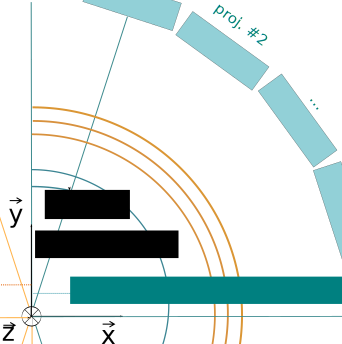
\includegraphics[width=0.4\columnwidth]{./figures/spect_angles.pdf}
  \caption{Projections angles conventions for a multi-headed SPECT system, in the regular (clockwise) orientation.}
  \label{fig_SPECT_angles}
\end{figure}


\paragraph{Optional fields}
\begin{itemize}
  \item \textbf{Zoom}: The zoom applied during the acquisition, for monolithic detectors. It is used to restric the effective size of the detector in both transaxial and axial directions inside which the acquisition bins are included (so this affect the size of the bins) (default: 1.)
  \item \textbf{Number of bins}: The transaxial and axial number of bins, separated by a comma. (default: if number of bins are not provided in the datafile header, the transaxial/axial number of pixels as defined in the .geom scanner configuration file are used instead)
  \item \textbf{Head rotation direction}: Rotation direction of the head(s). Must be either clockwise (\textit{CW}, defaut) or counter-clockwise \textit{(CCW)}.
  \item \textbf{Calibration factor}: The calibration factor associated to the current scanner settings (default: 1.)
  \item \textbf{Normalization correction flag}: Specify if the binary datafile contains normalization correction factors (default: 0 = no ; 1 = yes)
  \item \textbf{Scatter correction flag}: Specify if the binary datafile contains scatter correction factors (default: 0 = no ; 1 = yes)
%  \item \textbf{Event kind flag}: Specify if the binary datafile contains an information tag (used only for list-mode data) (default: 0 = no ; 1 = yes)
  \item \textbf{Isotope}: Isotope used during the acquisition (currently not taken into account)
\end{itemize}

The two following fields are optional but if used, then only one must appear. If none is provided, then the global distance from camera surface
to the center of rotation is taken from the SPECT system geometric description file, and assumed constant for all projections.
\begin{itemize}
  \item \textbf{Global distance camera surface to COR}: Global distance in mm between the detector surface and the center of rotation (this distance must be constant for all projections)
  \item \textbf{Distance camera surface to COR}: Distance in mm between the detector surface and the center of rotation, for each projection angle (separated by commas). For a multiheaded SPECT system, the distances for each projection angle of the first head must be provided first, followed by the distances of each projection angles of the 2$^{nd}$ head, \textit{etc}.

This field expect a number of entries equal to the total number of projection angles (for each head), even if the distances are constant. For example, the list of COR to detector distances for the system displayed in Fig. \ref{fig_SPECT_angles} must be:\\
$CORd_{h1}$, $CORd_{h1}$, $CORd_{h1}$, $CORd_{h1}$, $CORd_{h1}$, $CORd_{h1}$, $CORd_{h1}$, $CORd_{h1}$, $CORd_{h1}$, $CORd_{h1}$, $CORd_{h2}$, $CORd_{h2}$, $CORd_{h2}$, $CORd_{h2}$, $CORd_{h2}$, $CORd_{h2}$, $CORd_{h2}$, $CORd_{h2}$, $CORd_{h2}$, $CORd_{h2}$

\end{itemize}

%---------------------------------------------------------------------------------------------------------------------------------------------------------------
\subsubsection{Binary datafile}

Tables \ref{table_SPECT_conv_data_bin_histogram} and \ref{table_SPECT_conv_data_bin_list-mode} describe the binary content of an event from a histogram and
list-mode binary datafile, respectively. Note that little endian encoding only is supported. Whether an optional data field is present or not, the order of
the fields provided in these tables must be observed. The meaning of the type \textit{FLTNBDATA} is explained in section~\ref{s_install}. The projection and
bin IDs are linked to the SPECT parallel/convergent geometry description used for the scanner associated to the datafile (see
section~\ref{ss_scanner_integration_SPECT_conv}).

\begin{table} [h!]
  \small
  \caption{Mandatory/Optional fields of a parallel/convergent SPECT histogram event}
  \label{table_SPECT_conv_data_bin_histogram}
  \begin{center}
  \begin{tabular}{|c|c|c|c|c|}
  \hline
   & \textbf{Symbol} & \textbf{Description} & \textbf{Type} & \textbf{Mandatory}\\
  \hline
  \hline
  1 & t & Time in ms & uint32\_t & yes \\ \hline
  2 & p & Amount of data in the bin & FLTNBDATA & yes \\ \hline
  3 & s & Un-normalized scatter intensity rate & FLTNBDATA & no \\ 
  & & of the corresponding histogram bin (count/s) & &  \\ \hline
  4 & n & Normalization factor of the corresponding histogram bin & FLTNBDATA & no \\ \hline
  5 & v & Projection ID (angular view) & uint32\_t & yes \\ \hline
  6 & c & Bin ID & uint32\_t & yes \\ \hline
  \end{tabular}
  \end{center}
\end{table}

\begin{table} [h!]
  \small
  \caption{Mandatory/Optional fields of a parallel/convergent SPECT list-mode event}
  \label{table_SPECT_conv_data_bin_list-mode}
  \begin{center}
  \begin{tabular}{|c|c|c|c|c|}
  \hline
   & \textbf{Symbol} & \textbf{Description} & \textbf{Type} & \textbf{Mandatory}\\
  \hline
  \hline
  1 & t & Time in ms & uint32\_t & yes \\ \hline
  2 & s & Un-normalized scatter intensity rate & FLTNBDATA & no  \\
   & & of the corresponding event (count/s) &  & \\ \hline
  3 & n & Normalization factor of the corresponding event & FLTNBDATA & no \\ \hline
  4 & v & Projection ID (angular view) & uint32\_t & yes \\ \hline
  5 & c & Bin ID & uint32\_t & yes \\ \hline
  \end{tabular}
  \end{center}
\end{table}

%---------------------------------------------------------------------------------------------------------------------------------------------------------------
%---------------------------------------------------------------------------------------------------------------------------------------------------------------
\newpage
\subsection{CT datafile format}
\label{ss_input_CT}

By CT data, we mean data linked to a CT geometry as described in section~\ref{ss_scanner_integration_CT}.
CT datafiles can hold histogram data with associated corrections (list-mode format is to be developed).
Note that CASToR will reconstruct transmission images in cm$^{-1}$ as it is the common unit of attenuation values in physics.

%---------------------------------------------------------------------------------------------------------------------------------------------------------------
\subsubsection{ASCII header}

The content of the ascii header file is described below. It includes mandatory and optional fields. All keywords are case sensitive and the
separator (between the field and the value) is the colon sign ":".


\paragraph{Mandatory fields}
\begin{itemize}
  \item \textbf{Scanner name}: The name of the CT scanner (corresponding to a scanner in the \textit{config/scanner} folder, without
        the file extension)
  \item \textbf{Data filename}: The absolute or relative path to the binary datafile
  \item \textbf{Number of events}: The number of CASToR events in the binary datafile
  \item \textbf{Data mode}: Can be "list-mode" or "histogram"
  \item \textbf{Data type}: CT
  \item \textbf{Start time (s)}: The relative start time of the acquisition in seconds
  \item \textbf{Duration (s)}: The duration of the acquisition in seconds
  \item \textbf{Number of projections}: The total number of projections in the acquisition (considering all the heads)
\end{itemize}

The positions of the projections can be provided with one of the two following mandatory options:

\begin{itemize}
  \item \textbf{Projection angles}: Angles in degrees for each projection, separated by commas.
  \item \textbf{First and last projection angles}: First and last included angles, then all projection angles are computed from them and the scanner rotation direction.
\end{itemize}

\paragraph{Optional fields}
\begin{itemize}
  \item \textbf{Scanner rotation direction}: Rotation direction of the head(s). Must be either clockwise (\textit{CW}, defaut) or counter-clockwise \textit{(CCW}).
  \item \textbf{Scatter correction flag}: Specify if the binary datafile contains scatter correction factors (default: 0 = no ; 1 = yes)
  \item \textbf{Blank correction flag}: Specify if the binary datafile contains blank measurements (default: 0 = no ; 1 = yes)
\end{itemize}

%---------------------------------------------------------------------------------------------------------------------------------------------------------------
\subsubsection{Binary datafile}

Table \ref{table_CT_data_bin_histogram} describe the binary content of an event from a histogram binary datafile.
Note that little endian encoding only is supported. Whether an optional data field is present or not, the order of
the fields provided in these tables must be observed. The meaning of the type \textit{FLTNBDATA} is explained in section~\ref{s_install}. The projection and
pixel IDs are linked to the CT geometry description used for the scanner associated to the datafile (see section~\ref{ss_scanner_integration_CT}).

\begin{table} [h!]
  \small
  \caption{Mandatory/Optional fields of a CT histogram event}
  \label{table_CT_data_bin_histogram}
  \begin{center}
  \begin{tabular}{|c|c|c|c|c|}
  \hline
   & \textbf{Symbol} & \textbf{Description} & \textbf{Type} & \textbf{Mandatory}\\
  \hline
  \hline
  1 & t & Time in ms & uint32\_t & yes \\ \hline
  2 & y & Amount of data in the bin & FLTNBDATA & yes \\ \hline
  3 & s & Scatter intensity rate & FLTNBDATA & no \\ 
  & & of the corresponding histogram bin (count/s) & &  \\ \hline
  4 & b & Blank measurement of the corresponding histogram bin & FLTNBDATA & no \\ \hline
  5 & v & Projection ID (angular view) & uint32\_t & yes \\ \hline
  6 & c & Pixel ID & uint32\_t & yes \\ \hline
  \end{tabular}
  \end{center}
\end{table}





%---------------------------------------------------------------------------------------------------------------------------------------------------------------
%---------------------------------------------------------------------------------------------------------------------------------------------------------------
%---------------------------------------------------------------------------------------------------------------------------------------------------------------
%                D Y N A M I C     R E C O N S T R U C T I O N
%---------------------------------------------------------------------------------------------------------------------------------------------------------------
%---------------------------------------------------------------------------------------------------------------------------------------------------------------
%---------------------------------------------------------------------------------------------------------------------------------------------------------------
\clearpage
\section{Dynamic reconstruction}
\label{s_dynamic}

CASToR implements different command line options in order to manage dynamic datafiles. The temporal splitting of a dynamic acquisition can be customized with the "\textit{-frm}" option. Likewise, the images of a gated acquisition can be independently reconstructed using "\textit{-g}". These options are presented below. Note that information about these command-line options presented below can also be displayed from the code executable using the option \textit{-help-dynamic}.

\subsection{Framing (-frm)}
This option allows to split the dataset in time frames whose duration is defined by the user. When enabled, a different image will be reconstructed for each time frame. The attribution of each data element (line of response for list-mode, or histogram bin) to a specific frame is performed using the \textit{timestamp} of each event. These events are assumed to be chronologically ordered in the dataset (both for list-mode and histogram). In the latter case, the 4D dataset of 3D histograms, each belonging to a frame, is supposed to be chronologically concatenated and in this case the framing definition used for binning the histograms should be used as input for -frm, except if gating is involved (see next paragraph below).

The time splitting of the data could be provided to the main code with the command line option -frm list, where 'list' is a list of frame start times, separated with commas (default: 1 frame of the whole input file duration). Duration for each frame can also be specified using a colon after the frame start time. When no duration is specified for a frame, the duration will be set equal to the difference between the start of this frame and the next one (assuming no gap between frames). It is mandatory though to specify the duration of the last frame. \\
Add 's' or 'm' to each frame start time or duration to specify if values are seconds or minutes (seconds is the default if none provided). The maximum precision of frames is milliseconds. \textit{e.x.} for a 35 minutes aquisition to 9 frames, starting with two frames of 50 seconds duration \\ -frm 0:50,60:50,2m,5m,10m,15m,20m,25m,30m:5m.

Figure \ref{fig_framing_list} presents the dynamic splitting of a list-mode data with two different dynamic protocols. The green one \textit{-frm 0,30,60,90:30} splits the dataset in 30s frames. The red one \textit{-frm 30,40:10,60,90:20} set a delay of 30 seconds before the 1st frame. 2nd and last frames are 10 seconds and 20 seconds long respectively. Lines of response whose timestamp is outside these frames are ignored.

%Todo : say that some changes may occur regarding  the new definition of histogram (now separated in 3D datafiles).
\bigskip
\begin{figure} [h!]
\centering
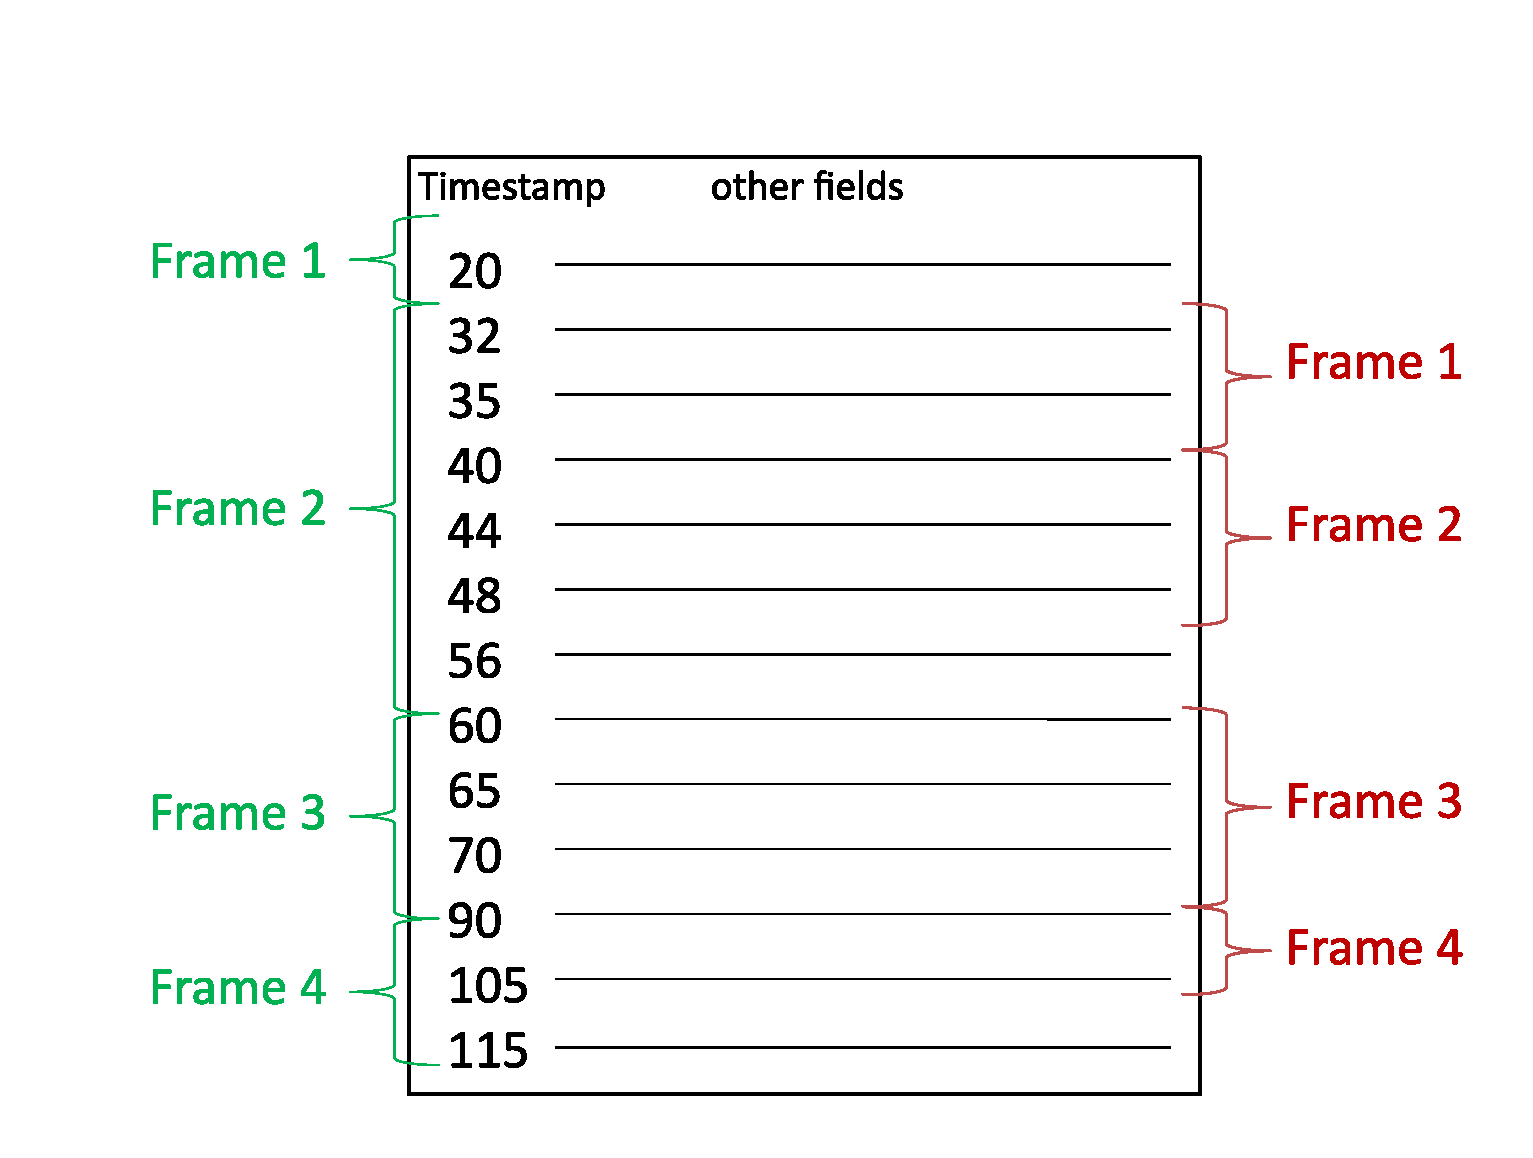
\includegraphics[width=0.49\columnwidth]{./figures/dynamic_framing_list.eps}
\caption{Example of frame splitting of a list-mode dynamic dataset with \textcolor{green}{\textit{-frm 0,30,60,90:30} (green)} and \textcolor{red}{\textit{-frm 30,40:10,60,90:20} (red)}}
\label{fig_framing_list}
\end{figure}

\bigskip

For histogram dataset, the histogram corresponding to each frame must be first processed according to the dynamic protocols requirement, and concatenated. Currently, the timestamp of each events will be used to identify each frame (each event inside a histogram must have the same timestamp). Figure \ref{fig_framing_hist} present the dynamic splitting of a histogram dataset with the two previous dynamic protocols. 


\begin{figure} [h]
  \centerline
  {
    \subfigure[\textcolor{green}{\textit{-frm 0,30,60,90:30}}]{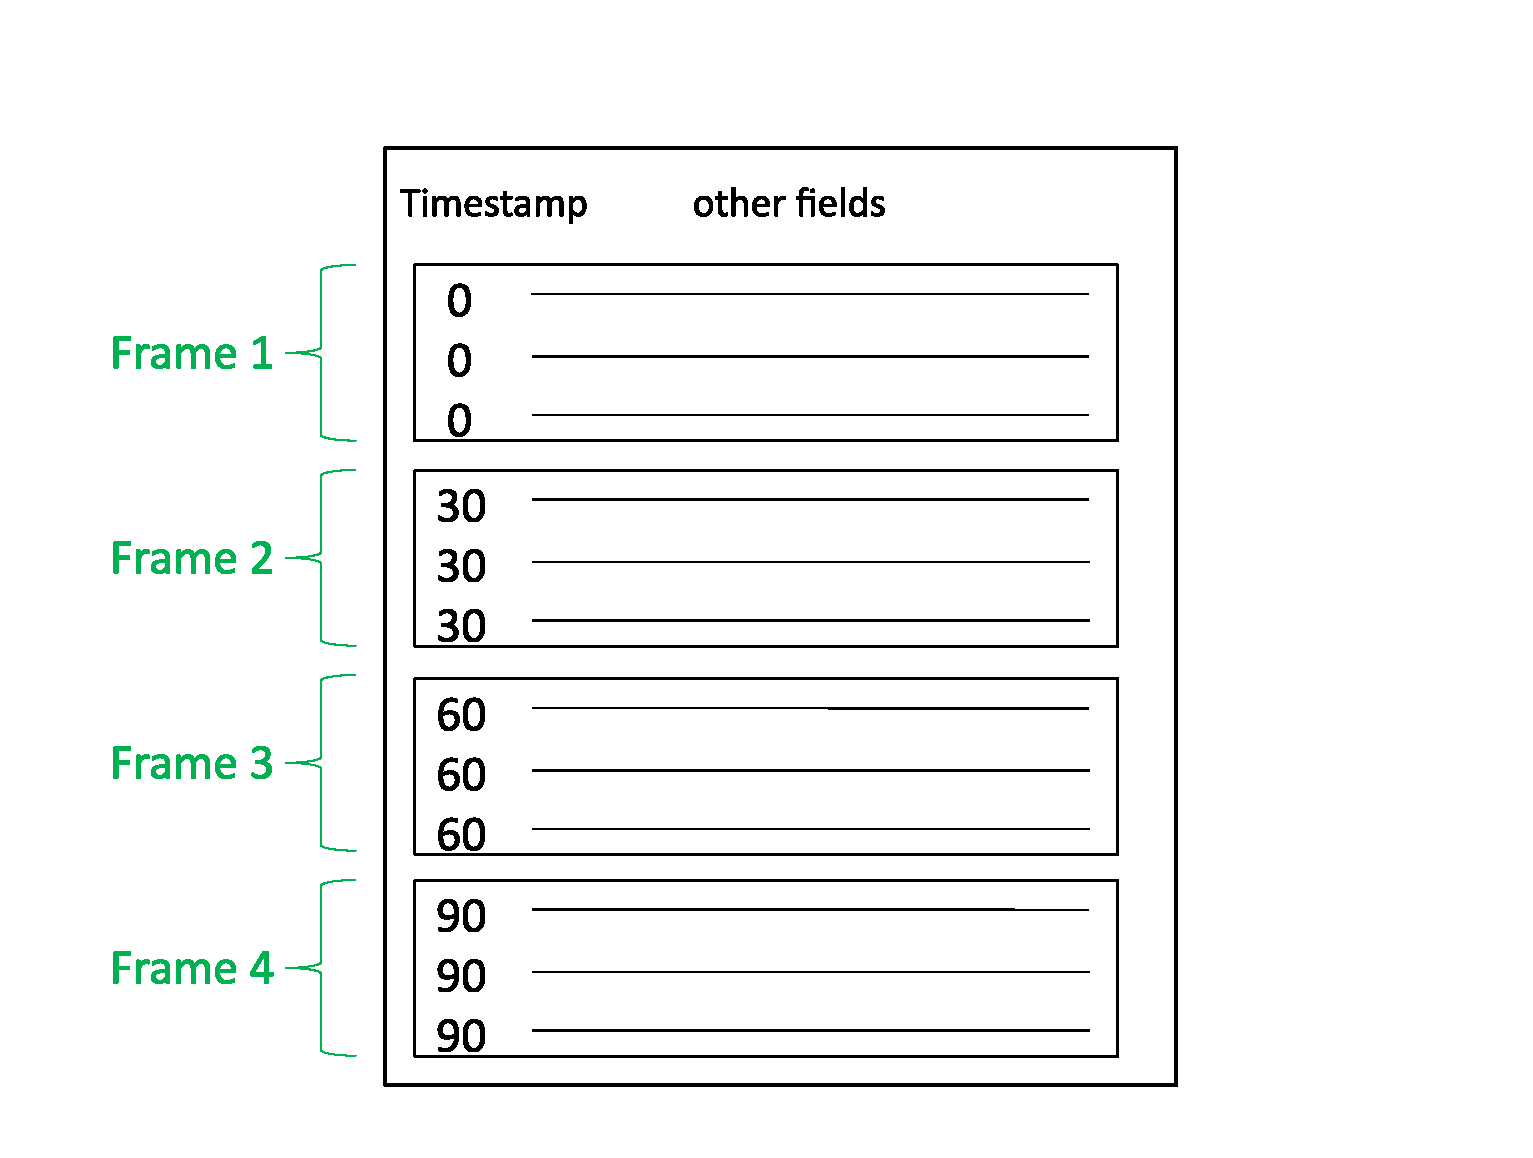
\includegraphics[width=0.49\columnwidth]{./figures/dynamic_framing_hista.eps}
    \label{fig_framing_hist_a}}
    \subfigure[\textcolor{red}{\textit{-frm 30,40:10,60,90:20}}]{\includegraphics[width=0.49\columnwidth]{./figures/dynamic_framing_histb.eps}
    \label{fig_framing_hist_b}}
  }
  \caption{Example of frame splitting of histogram dynamic datasets with different frame duration configurations.}
  \label{fig_framing_hist}
\end{figure}




\subsection{Gating (-g) and time-based operations}

%Physiological motion includes respiratory and cardiac motions. Due to the cyclic nature of these motions, the CASToR implementation requires a specific organization of the datafile. The following points details the requirements on the dataset and on the characterization of the motion parameters.

A dynamic dataset can also be splitted into different parts, either on a chronological basis (time-based motion correction), or depending on specific numbers of events (gated dataset). Typical applications is the reconstruction of a respiratory or cardiac gated acquisition, or image-based motion correction. 


\subsubsection{Gated dataset}

This section assumes that the events in the dataset have previously been reorganized into \textit{gates}, i.e the events belonging to a same gate have been grouped together. For list-mode data, this assumes that the line of responses are no more chronologically stored, but are sorted by gate. For histogram dataset, this implies that the events have been rebinned in different histograms, each corresponding to one gate. In the current CASToR implementation, the data contained in each gate (group of lines of response for list-mode, or gated histograms) must be concatenated. This is illustrated by figure \ref{fig_gating}.



\begin{figure} [h]
  \centerline
  {
    \subfigure[Original list-mode]{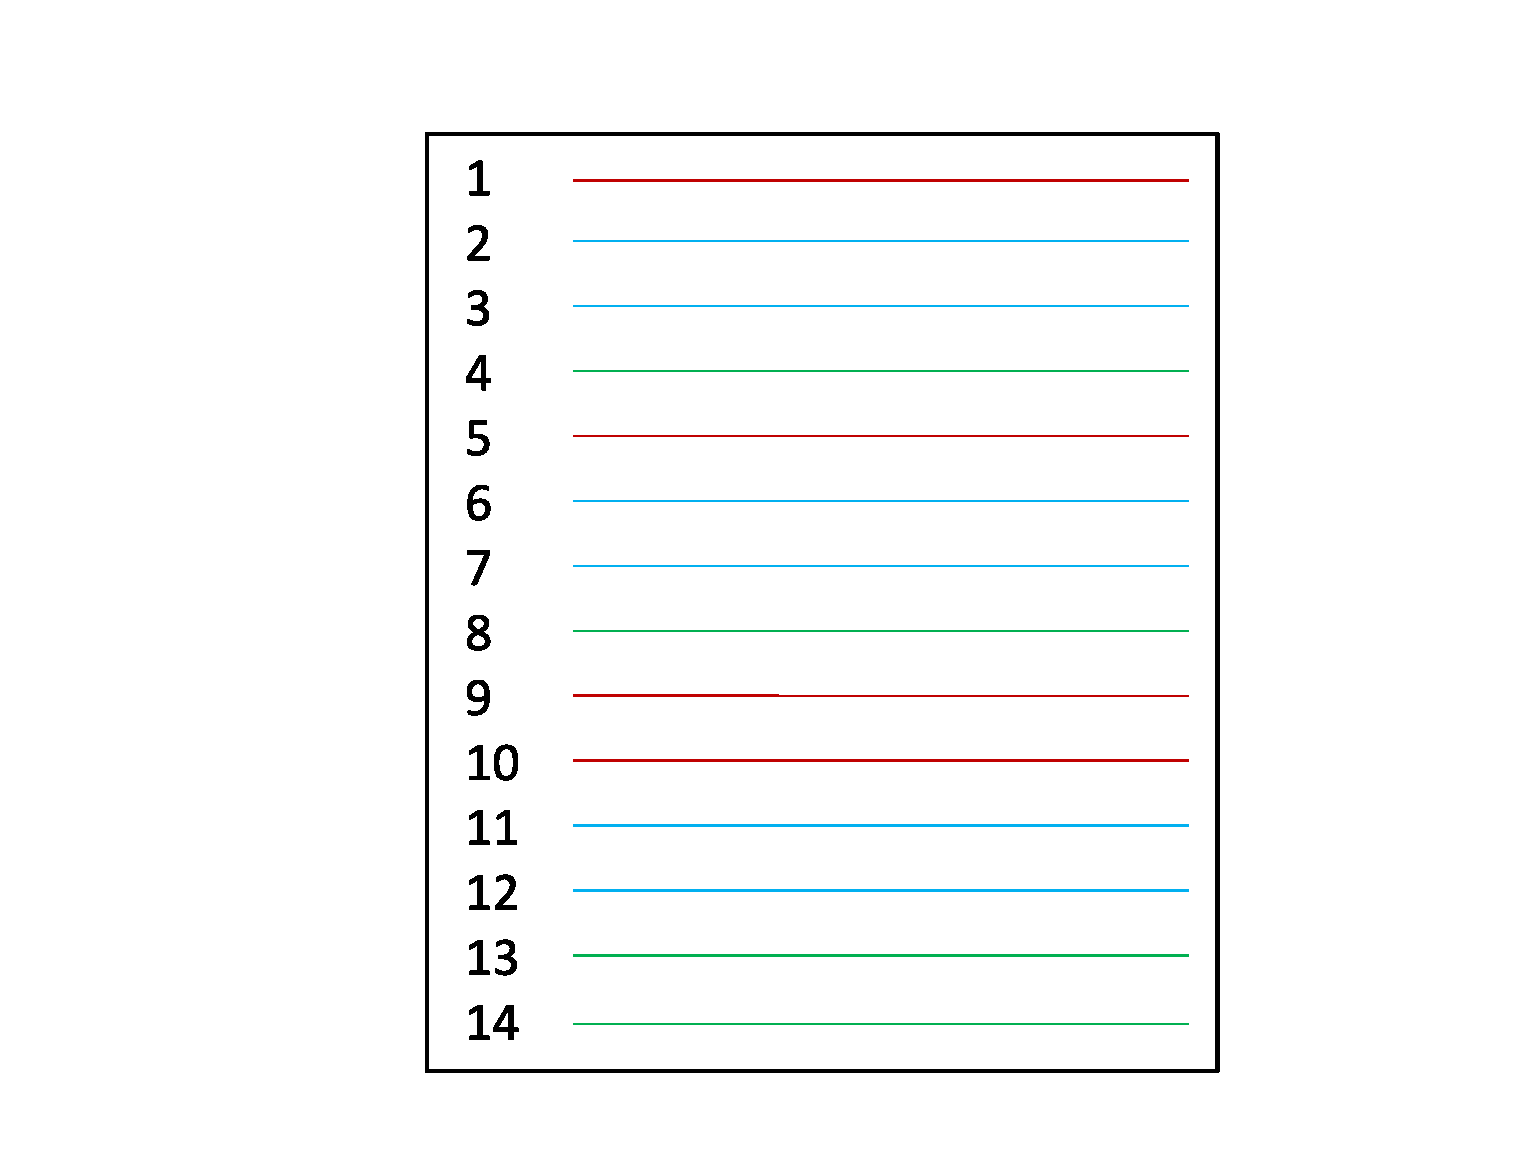
\includegraphics[width=0.33\columnwidth]{./figures/dynamic_original_list.eps}
    \label{fig_gating_a}}
    \subfigure[Gated list-mode]{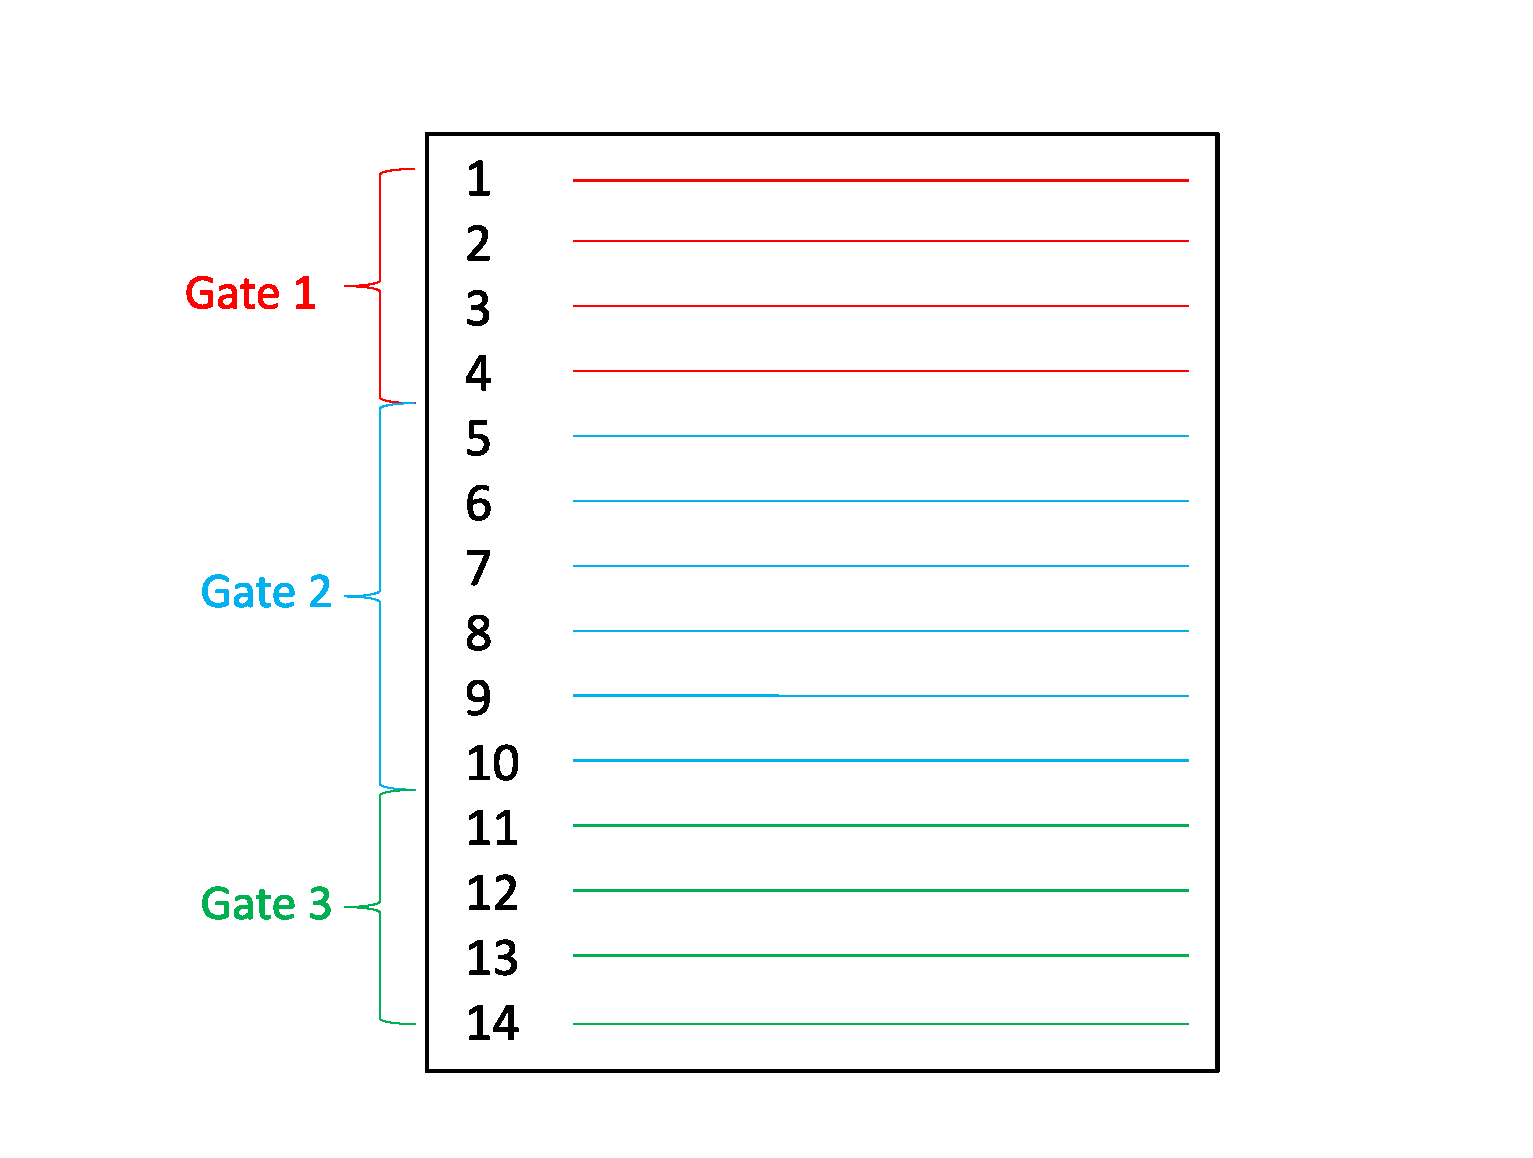
\includegraphics[width=0.33\columnwidth]{./figures/dynamic_gated_list.eps}
    \label{fig_gating_b}}
    \subfigure[Gated histogram(s)]{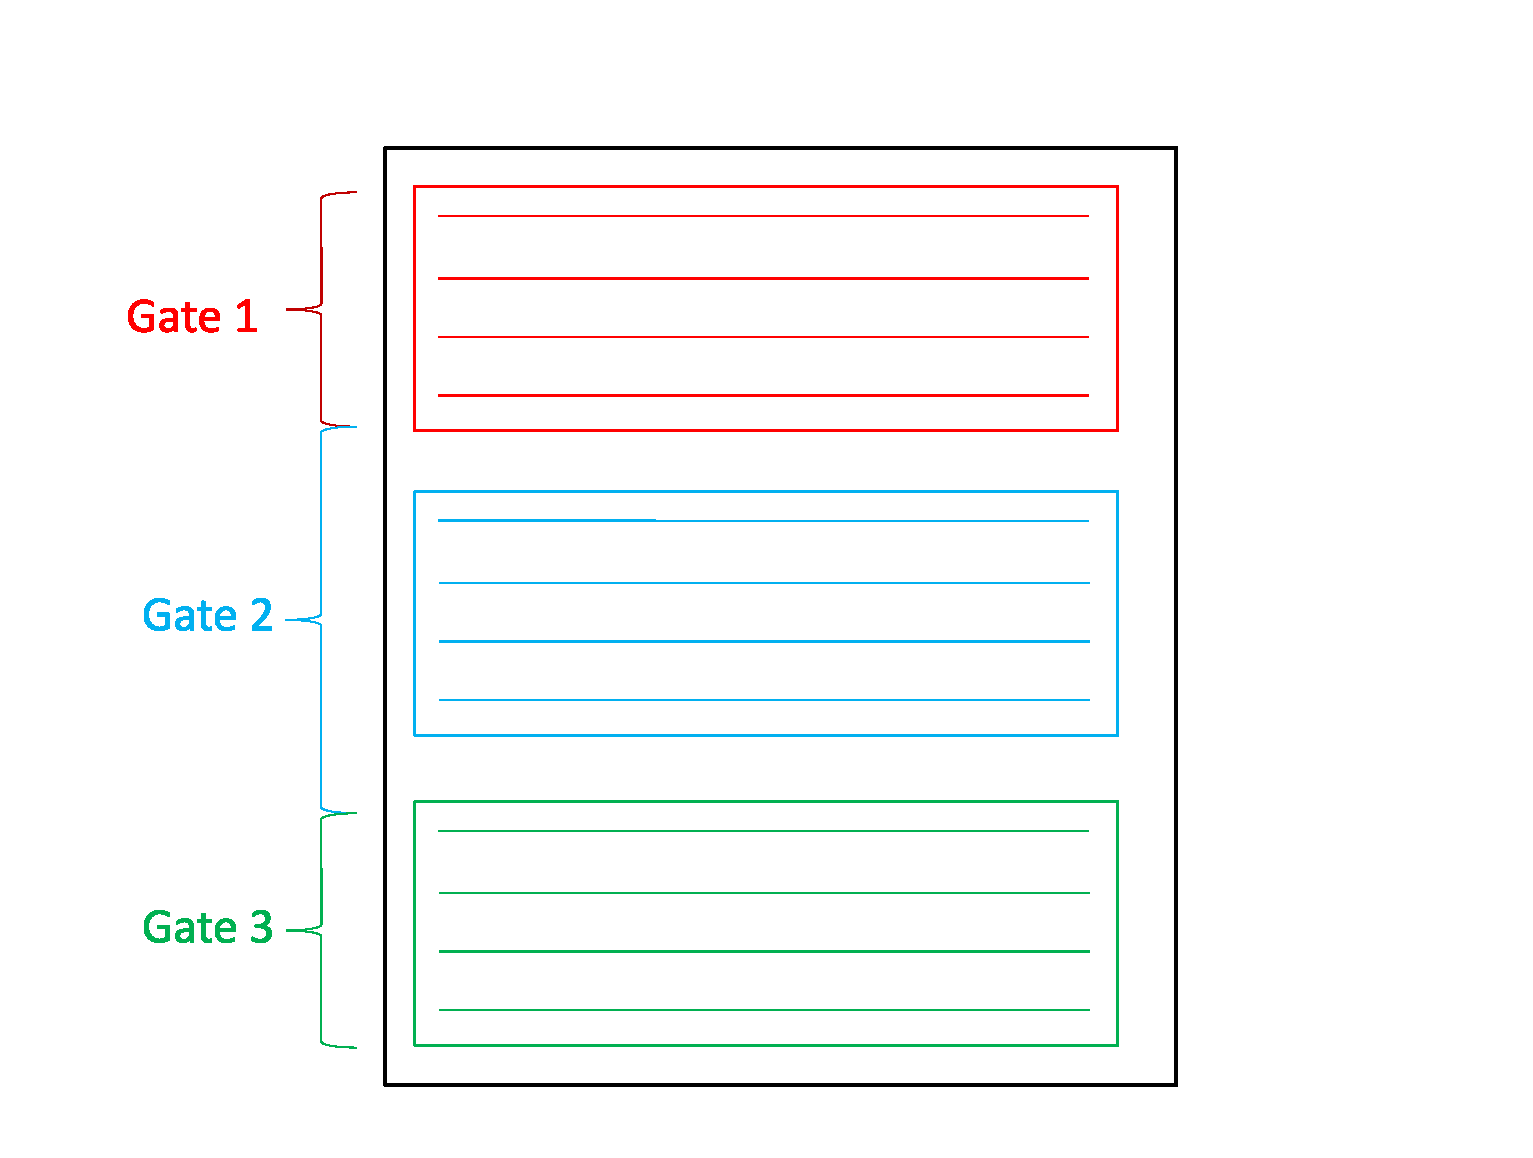
\includegraphics[width=0.33\columnwidth]{./figures/dynamic_gated_hist.eps}
    \label{fig_gating_c}}
  }
  \caption{Gating. Original list-mode dataset with chronologic sorting of line of response (left). Colors represent events belonging to a similar gate. Gated list-mode dataset (middle). Gated histogram dataset (right).}
  \label{fig_gating}
\end{figure}


% --- configuration file --- 

This option can be used to reconstruct separated images for each gate, or to apply image-based correction such as motion correction between each gate or time-subset.

Several information regarding the gating of the data have to be provided in the reconstruction command-line options using the \textbf{-g} option  along with a text file containing gating information in order to enable gating management. The required information are the number of respiratory/cardiac gates, and the number of data elements (events) inside each gates. These informations must be provided from a configuration file (\textit{-g path/to/configuration/file}). 

Listing \ref{list_gating} presents an example of a gating configuration file for a dynamic dataset containing 8 (respiratory) gates. The number of events in each gate are separated by commas. Using the \textbf{-g} command-line option and this set up, an image will be reconstructed for each gate within each frame.


\begin{lstlisting}[label={list_gating},caption= Setup of a gating file related to a dynamic dataset with respiratory gating.]

   nb_respiratory_gates: 8
   
   nb_events_respiratory_gates: 
   2908079, 2898161, 2890348, 2896543, 2895697, 2909393, 2897784, 2860467

\end{lstlisting}    


\paragraph{Quantification for independent gate reconstruction:} If the gates are independently reconstructed (no motion correction), a quantification factor is computed by default for each gate according to their number of events and the number events of the frame (or the entire acquisition) they belong to. This assumes that counts must be balanced between the different gates. Alternatively, one could optionally provide duration for each gate with the \textit{duration\_gate} keyword like in the following example. Unit must be seconds.

\begin{lstlisting}[label={list_gating},caption= Setup of a gating file related to a dynamic dataset with respiratory gating.]

   nb_respiratory_gates: 8
   
   nb_events_respiratory_gates: 
   2908079, 2898161, 2890348, 2896543, 2895697, 2909393, 2897784, 2860467

   duration_gate: 
   35,36.5,39,40,40,38,36,35.5
\end{lstlisting}    

If dynamic frames are present, the gate durations must be provided on a different line for each frame. If both respiratory and cardiac gates are present, the duration for each cardiac gates must be provided (thus assuming a respiratory gate contains several cardiac gates).

% --- 5+D datasets --- 
\bigskip

For 5+D datasets (containing dynamic frames and gates), the gates must be concatenated within each frame. The timestamp of the lines of response / histogram events will be still used to split the frames. Figure \ref{fig_gating_5D} illustrates how a 5D list-mode including 3 frames and 3 gates must be organized with CASToR ). Regarding the configuration file, the gating associated to each frame must be entered on a separate line. Listing \ref{list_gating_5D} illustrates the configuration file related to this sample dataset.


\bigskip
\begin{figure} [h!]
\centering
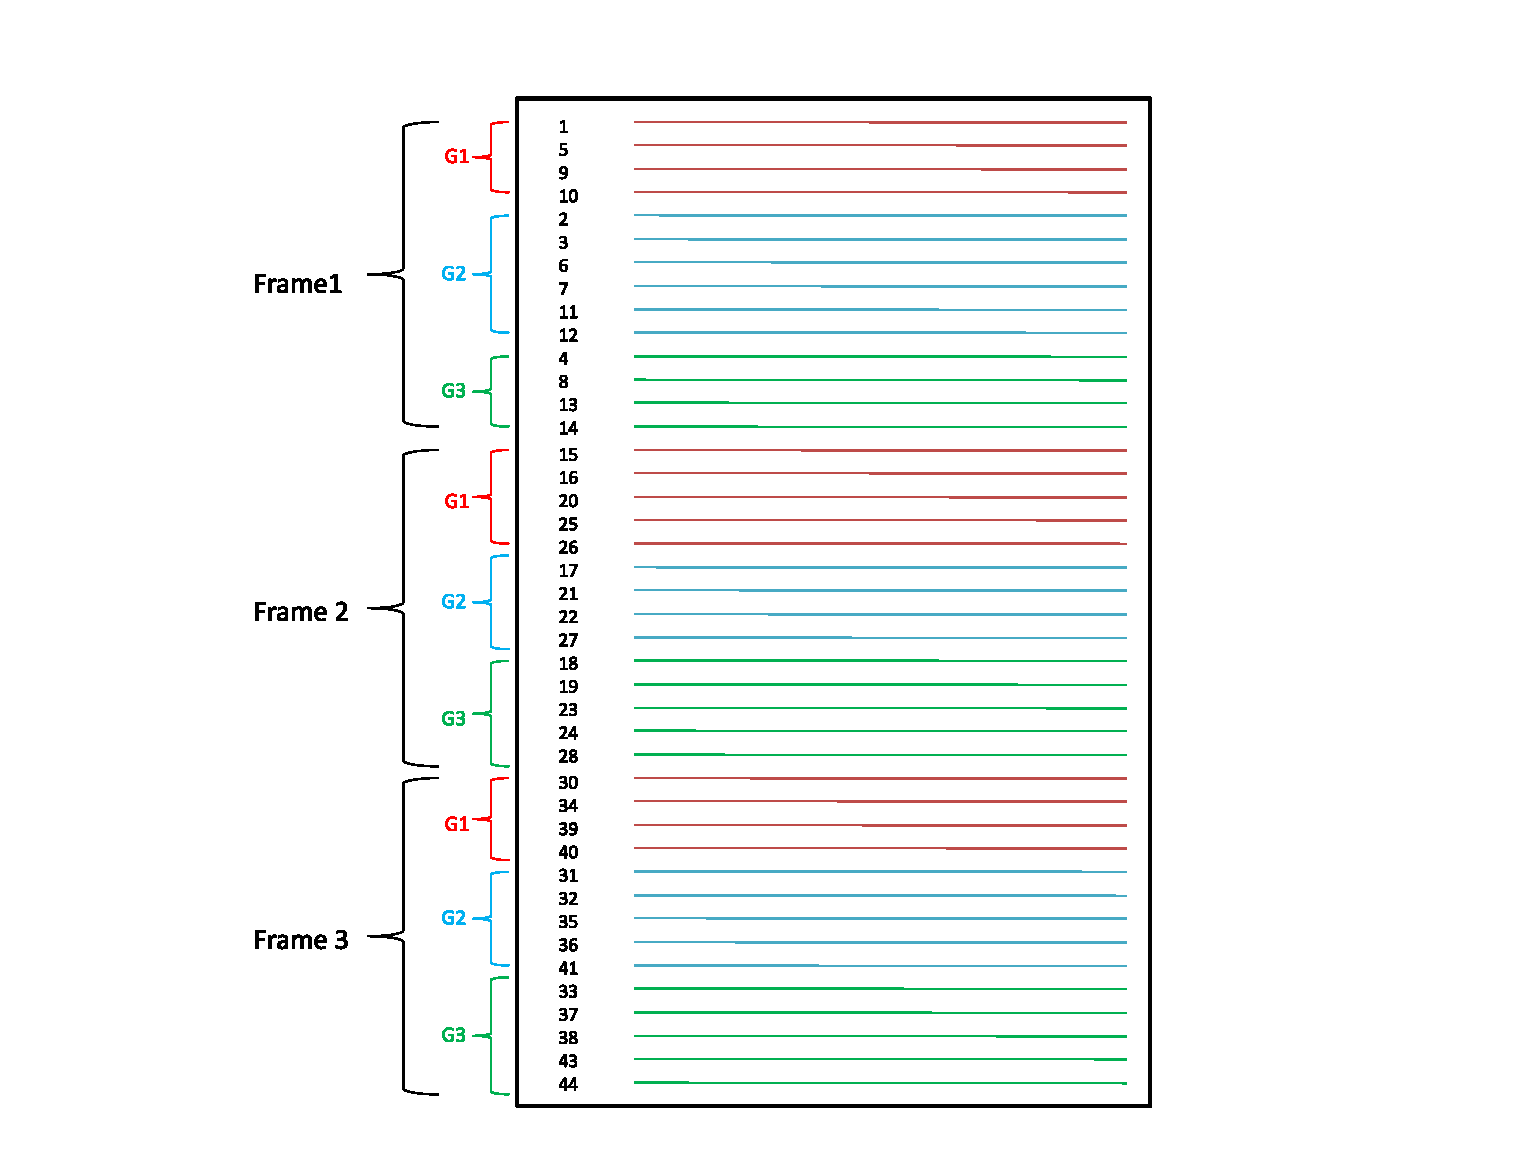
\includegraphics[width=0.49\columnwidth]{./figures/dynamic_gated_5D.eps}
\caption{Example of splitting of a 5D dynamic gated dataset.}
\label{fig_gating_5D}
\end{figure}


\begin{lstlisting}[label={list_gating_5D},caption= Setup of the gating file related to the dynamic dataset in figure \ref{fig_gating_5D}).]

   nb_respiratory_gates: 3
   
   nb_events_respiratory_gates: 
   4,6,4
   5,4,5
   4,5,5

\end{lstlisting}    


% --- physiological motion ---
Physiological motion can be addressed using image-based motion correction. If a gated dataset is associated with respiratory or cardiac motion correction (rm, cm), image-based deformation will be applied between the subsets to correct the images for motion. More details about the deformation module are provided in the \textit{CASToR\_\_image\_deformation} pdf document.
 

\bigskip
\subsubsection{Time-based motion correction}


A dataset can be corrected from accidental motion (patient head/body motion) during reconstruction by providing the timestamps in which the motion correction must be applied, and transformation parameters. To enable time-based motion correction, a file must be given to castor-recon through the -g option, with the following keywords:

\begin{itemize}
\item \textbf{nb\_motion\_triggers: x}  

Total number \textit{x} of time-based motion trigger in the acquisition. 
   
\item \textbf{timestamp\_motion\_triggers: list } 

List of timestamp in seconds, for which the transformations must be performed. Each timestamp must be separated by a comma.
          
\end{itemize}

Listing \ref{list_pmotion_init} presents an example if time-based motion configuration file. Note that as transformation parameters must be provided for each sub-division of the dataset, the first timestamp must be the 0 (seconds). As usually the start of the acquisition is defined as the reference position, the transformation parameters associated with the first motion should be set to identity (i.e, no transformation). Each timestamp will be associated with a deformation model which must be initialized with the \textit{-im} option. More details about the deformation models are provided in the \textit{CASToR\_\_image\_deformation} pdf document.


\begin{lstlisting}[label={list_pmotion_init},caption= Example of time-based motion keyword initialization.]

   DYNAMIC FRAMING
   nb_motion_triggers: 6
   
   timestamp_motion_triggers: 0, 2280, 2460, 3060, 3180, 3480

\end{lstlisting}    







%---------------------------------------------------------------------------------------------------------------------------------------------------------------
%---------------------------------------------------------------------------------------------------------------------------------------------------------------
%---------------------------------------------------------------------------------------------------------------------------------------------------------------
%                I M A G E   F I L E   F O R M A T
%---------------------------------------------------------------------------------------------------------------------------------------------------------------
%---------------------------------------------------------------------------------------------------------------------------------------------------------------
%---------------------------------------------------------------------------------------------------------------------------------------------------------------
\clearpage
\section{Image file format}
\label{s_interfile}

CASToR uses the Interfile format for image reading and writing. The format consists in a binary image file associated with an ASCII header (text file)
containing metadata about the image (image location, dimensions, voxel size, etc). The header being easy to read and edit without specific tools,
this format is very flexible and can handle different type of images, given that the adequate keys are provided. For a suggestion of softwares to read \castor reconstructed images, please see section \ref{ss_quickstart_readImages}.

%---------------------------------------------------------------------------------------------------------------------------------------------------------------
%---------------------------------------------------------------------------------------------------------------------------------------------------------------
\subsection{Supported keys}
\label{ss_intf_keys}

A limited number of keys are actually required to read/write an image in order to simplify the conversion from another image format to Interfile,
and conversely. An Interfile key is based on key/value pairs such as \textit{key := value}. 

The header must be located in the same directory as the image file. The minimal interfile header must provide the image path, the image dimensions, the
voxel size and the image encoding, as in this example:

\begin{lstlisting}[label={intf3D},caption= Interfile header mandatory keys for reading]
  !name of data file := img_name.img
  !total number of images := 47
  imagedata byte order := LITTLEENDIAN
  number of dimensions := 3
  !matrix size [1] := 256
  !matrix size [2] := 256
  !matrix size [3] := 50
  !number format := short float
  !number of bytes per pixel := 4
  scaling factor (mm/pixel) [1] := 4
  scaling factor (mm/pixel) [2] := 4
  scaling factor (mm/pixel) [3] := 4
  image duration (sec) := 1
\end{lstlisting}
 
Below are listed the supported keys in the current version:

\begin{itemize}
  \item "name of data file" : name of the image binary file
  \item "imagedata byte order" : endianness (must be LITTLEENDIAN or BIGENDIAN)
  \item "data starting block" : Data offset in block of 2048 bytes
  \item "data offset in bytes" : Data offset using a provided number of bytes
  \item "number format" : Type of each pixel/voxel data (must be 'long float', 'short float', 'signed integer', 'unsigned integer')
  \item "number of bytes per pixel" : Number of bytes for each pixel/voxel of the image data
  \item "matrix size [1]" : Width (number of voxels) (x-axis dimension)
  \item "matrix size [2]" : Height (number of voxels) (y-axis dimension)
  \item "matrix size [3]" : Slices (number of voxels) (z-axis dimension)
  \item "matrix size [4]" : number of (dynamic) time frames
  \item "scaling factor (mm/pixel) [1]"  : Width voxel size
  \item "scaling factor (mm/pixel) [2]"  : Height voxel size
  \item "scaling factor (mm/pixel) [3]"  : Axial voxel size
  \item "slice thickness (pixels)" : slice thickness, assumed to be provided in mm regardless of the name.
        'scaling factor (mm/pixel) [3]' has the priority over this field. If it is not provided, the axial voxel size is computed as (scaling
        factor (mm/pixel) [1] + scaling factor (mm/pixel) [2]) / 2.) * slice thickness (pixels)
  \item "number of time frames" : number of (dynamic) time frames. Priority over "matrix size [4]"
  \item "number of respiratory gates" : (CASToR key) number of respiratory gated images
  \item "number of cardiac gates" : (CASToR key) number of cardiac gated images
  \item "rescale slope" : calibration factor
  \item "quantification units" : calibration factor (cumulative to "rescale slope"). If this field provids unit (eg : kbq/cc), it is simply ignored
  \item "rescale intercept" : additive calibration value
  \item "study duration (sec)" : acquisition duration in seconds 
  \item "image duration (sec)" : image duration in seconds
  \item Image positionning of offset related keys such as "origin (mm) [x]', 'offset [x]', 'first pixel offset (mm) [x]' are not supported in
        the current version, which assumes that all images are centered in the field of view.
  \item Image orientation related keys such as 'slice orientation', 'patient rotation', 'patient orientation' are ignored in the current version,
        as such information is most of the time missing and/or misleading.
\end{itemize}

%---------------------------------------------------------------------------------------------------------------------------------------------------------------
%---------------------------------------------------------------------------------------------------------------------------------------------------------------
\subsection{Dynamic images}
\label{ss_intf_dynamic}

Dynamic images can be provided or written on disk through two formats: a metaheader associated to a series of Interfile images, and a single file
containing all the frames/gated images. Default output option for dynamic images is the metaheader.

%---------------------------------------------------------------------------------------------------------------------------------------------------------------
\subsubsection{Metaheader}
\label{sss_intf_dynamic_mhd}

The metaheader is an ASCII file gathering main information about the dynamic images, the actual number of images, and the path to each one of them.
Here is an example:

\begin{lstlisting}[label={intfMHD},caption= Interfile Metaheader mandatory keys for reading]
  number of time frames := 10
  number of respiratory gates := 1
  number of cardiac gates := 1
  ! total number of datasets:= 10
  %data set [1]:={0,img_frm0.hdr,UNKNOWN}
  %data set [2]:={0,img_frm1.hdr,UNKNOWN}
  %data set [3]:={0,img_frm2.hdr,UNKNOWN}
  %data set [4]:={0,img_frm3.hdr,UNKNOWN}
  %data set [5]:={0,img_frm4.hdr,UNKNOWN}
  %data set [6]:={0,img_frm5.hdr,UNKNOWN}
  %data set [7]:={0,img_frm6.hdr,UNKNOWN}
  %data set [8]:={0,img_frm7.hdr,UNKNOWN}
  %data set [9]:={0,img_frm8.hdr,UNKNOWN}
  %data set [10]:={0,img_frm9.hdr,UNKNOWN}
\end{lstlisting}

The metaheader must contain the following mandatory keys:

\begin{itemize}
  \item "total number of datasets" : number of associated files
  \item "data set [xxx]" : path to each interfile image header associated with the metaheader, where xxx represents a number
        starting from 1 (not 0). It must be an array key whose second element contains the path. The 1st and 3rd elements, respectively
        0 and UNKNOWN in the example) are ignored. The number of "data set [xxx]" must correspond to the value provided by the
        'total number of datasets' keys
  \item "number of time frames" : Number of dynamic frames (not required if the data does not contain any)
  \item "number of respiratory gates" : (CASToR key) Number of respiratory gated images (not required if the data does not contain any)
  \item "number of cardiac gates" : (CASToR key) Number of cardiac gated images (not required if the data does not contain any)
\end{itemize}

The header of the associated image files must be similar to standard Interfile header file as described by the listing \ref{intfMHD}.

%---------------------------------------------------------------------------------------------------------------------------------------------------------------
\subsubsection{Merged dynamic interfile}
\label{sss_intf_dynamic_merged}

The binary image file must contain all the frames and/or gated images concatenated into a single binary file. The associated header must
contain all information for each frame/gated image included in the binary image file, as in the example below (listing \ref{intfMerge4D}). No
information about the data offset position of each image is required.

By default, dynamic images will be written on disk as a metaheader associated with a separate interfile for each image. The command line
option "-omd" must be used to enable the output of dynamic images in one single file.

\begin{lstlisting}[label={intfMerge4D},caption= Interfile header of a dynamic image]
  !name of data file := img_name.img
  imagedata byte order := LITTLEENDIAN
  number of time frames := 10
  number of respiratory gates := 1
  number of cardiac gates := 1

  // Frame 1 
  imagedata byte order := LITTLEENDIAN
  !matrix size [1] := 256
  !matrix size [2] := 256
  !matrix size [3] := 50
  !number format := short float
  !number of bytes per pixel := 4
  scaling factor (mm/pixel) [1] := 4
  scaling factor (mm/pixel) [2] := 4
  scaling factor (mm/pixel) [3] := 4
  image duration (sec) := 10
  image start time (sec) := 0
  // Frame 2 
  imagedata byte order := LITTLEENDIAN
  !matrix size [1] := 256
  !matrix size [2] := 256
  !matrix size [3] := 50
  !number format := short float
  !number of bytes per pixel := 4
  scaling factor (mm/pixel) [1] := 4
  scaling factor (mm/pixel) [2] := 4
  scaling factor (mm/pixel) [3] := 4
  image duration (sec) := 10
  image start time (sec) := 10

  //(...)

  // Frame 10
  imagedata byte order := LITTLEENDIAN
  !matrix size [1] := 256
  !matrix size [2] := 256
  !matrix size [3] := 50
  !number format := short float
  !number of bytes per pixel := 4
  scaling factor (mm/pixel) [1] := 4
  scaling factor (mm/pixel) [2] := 4
  scaling factor (mm/pixel) [3] := 4
  image duration (sec) := 10
  image start time (sec) := 90
\end{lstlisting}


%---------------------------------------------------------------------------------------------------------------------------------------------------------------
%---------------------------------------------------------------------------------------------------------------------------------------------------------------
%---------------------------------------------------------------------------------------------------------------------------------------------------------------
%                C A S T O R   U T I L I T I E S
%---------------------------------------------------------------------------------------------------------------------------------------------------------------
%---------------------------------------------------------------------------------------------------------------------------------------------------------------
%---------------------------------------------------------------------------------------------------------------------------------------------------------------
\newpage
\section{CASToR utilities}
\label{s_utilities}

This part presents various utilities related to CASToR data processing, generation or conversion. Apart from the binary datafile converters (see section~\ref{ss_utilities_manufacturer}), the tools executables are located in the same directory than the main reconstruction program, while the source can be found in the toolkits/ directory from the main \castor repository. Compilation with CMake requires the two  CASToR\_BUILD\_GATE\_UTILITIES and CASToR\_BUILD\_SAMPLE\_UTILITIES options to be enabled in order to generate the executables. The use of the standard Makefile will automatically compile the toolkits. The toolkits currently include:
\begin{itemize}
\ifdefined\dev
  \item \textit{castor-proj}, an analytic projection utility, which generates a CASToR histogram datafile for a specific system, from a user-provided image \ref{ss_utilities_cproj}.
\fi
  \item GATE conversion utilities, to be used to generate a CASToR generic geometry file (geom) from a GATE macro file containing a \textit{cylindricalPET}
        or \textit{ecat} geometry and a CASToR datafile from a root file generated by GATE for these geometries. Subsection~\ref{ss_utilities_gate}.
  \item \textit{castor-PetScannerLutEx}, an example of a program which generates a geometric file containing a PET Look-Up-Table with information
        about the scanner elements, readable by CASToR. Subsection~\ref{ss_utilities_scriptLUT}.
  \item \textit{castor-datafileConversionEx}, an example of a program providing guidances on how to convert a datafile to the CASToR format.
        Subsection~\ref{ss_utilities_conversion}.
  \item \textit{castor-datafileExplorer}, which allows to get information about any \castor datafile and its content. Subsection~\ref{ss_utilities_dexplorer}.
  \item \textit{castor-scannerLUTExplorer}, which can be used to visualize a scanner Look-Up-Table (geometric position and orientation of the system crystals/pixels), element by element. Subsection~\ref{ss_utilities_sexplorer}.
  \item \textit{smc2castor} is an utility developed by Michael Ljungberg to convert SPECT projections simulated with the SPECT SIMIND Monte-Carlo program to CASToR file formats. \textit{smc2castor} can be found in SIMIND v6.1, available from the SIMIND website : (\url{https://www.msf.lu.se/forskning/the-simind-monte-carlo-program}).
\end{itemize}

%---------------------------------------------------------------------------------------------------------------------------------------------------------------
%---------------------------------------------------------------------------------------------------------------------------------------------------------------

\ifdefined\dev
\subsection{Analytic projection tool}
\label{ss_utilities_cproj}

\verb|castor-proj| is a basic analytic projection tool to compute a CASToR datafile from an user-provided image. It can be called through a
command line interface (shell or DOS-box) and launched with the correct set of options. Launching castor-proj without arguments will prompt
the main usage options. The following example presents a typical command line:

\bigskip
\verb|castor-proj(.exe) -img      path/to/input/image| 

\verb|                  -sc       system_alias| 

\verb|                  -dout     path/to/output/directory| 

  \verb|                  -fileType TYPE_PET -or- TYPE_SPECT| 
\bigskip

with the following options :

\begin{itemize}
  \item \textbf{-img}: path to the interfile image to project
  \item \textbf{-dout}: path to the output directory
  \item \textbf{-sc}: alias of the system to use for the projection
  \item \textbf{fileType \textit{type}}: give the type of events that will be generated: \textit{TYPE\_PET}, \textit{TYPE\_SPECT}.
        Default: \textit{TYPE\_PET}
\end{itemize}
\bigskip

Image spatial (and dynamic) dimensions are directly read from the image interfile header (see section \ref{s_interfile} for supported interfile fields).
The following commands display command options related to specific parts of the reconstruction algorithm 
 
\begin{itemize}
  \item \textbf{-help-in}: Input options (initialization,  attenuation, sensitivity images, etc..). 
  \item \textbf{-help-out}: Output options (output directory and images). 
  \item \textbf{-help-proj}: Specific help about projector settings. 
  \item \textbf{-help-comp}: Computational options (multithreading, RAM settings, etc..)
  \item \textbf{-help-dynamic}: Dynamic options for projection (config directory, verbosity, etc..)
  \item \textbf{-help-misc}: Miscellaneous options (config directory, verbosity, etc..)
  \item \textbf{-help-pet}: Specific help about PET settings for analytic projection.
  \item \textbf{-help-spect}: Specific help about SPECT settings for analytic projection.
  \item \textbf{-help-scan}: List of all systems available from the configuration directory projection.
  \item \textbf{-help-projm}: List and description of all implemented projectors.
\end{itemize}
\fi

%---------------------------------------------------------------------------------------------------------------------------------------------------------------
%---------------------------------------------------------------------------------------------------------------------------------------------------------------
\subsection{Binaries for manufacturer datafile conversion}
\label{ss_utilities_manufacturer}

Several executables able to convert manufacturer's datasets to a \castor datafile may be provided on the \castor website (see \url{http://www.castor-project.org/converters}).
Note that all these converters and associated materials are not supported nor validated by any manufacturer. Note also that the \castor software associated or not
with these converters is not approved for any medical use. The \castor developers and collaboration members cannot be responsible for any consequences
resulting from the use of any tool distributed on the \castor website.


%---------------------------------------------------------------------------------------------------------------------------------------------------------------
%---------------------------------------------------------------------------------------------------------------------------------------------------------------
\subsection{GATE utilities}
\label{ss_utilities_gate}

The GATE utilities use the macro files of a GATE simulation to generate the scanner geometry (as a CASToR .geom file \ref{sss_scanner_integration_PET_geom}),
and CASToR datafile (\ref{ss_input_PET}). These utilities currently have several limitations regarding the nature of the systems which can be converted:

\begin{itemize}
\item Supported GATE systems include \textit{cylindricalPET}, \textit{ecat}, and \textit{SPECThead} systems.
\item For PET systems, it is assumed that the first hierarchic level element (i.e rsector for \textit{cylindricalPET} and block for \textit{ecat}) use a ring repeater, while the other elements use either cubic or linear repeaters.
\item For SPECT systems, the specificities of the collimator aren't implemented.
\item Supported GATE output format is root.
\item Command positionning the first hierarchic level element (i.e: \textit{/gate/rsector/placement/setTranslation} ) must have a single non-zero component.
\item The script will look into the provided macro file, and the .mac file called from the given macro file, for GATE commands characterizing the system.
      Lines starting with a comment character ($\#$) are ignored.
\end{itemize}

There are currently two utilities: \textit{castor-GATERootToCastor} and \textit{castor-GATEMacToGeom}.

The \textit{castor-GATERootToCastor} program could be used to convert a ROOT list-mode datafile generated with GATE\cite{GATE} to a CASToR datafile.\\

Usage:\\

\verb|castor-GATErootToCastor(.exe) -i   path/to/ifile.root|

\verb|                                   (or)|

\verb|                              -il  path/to/ifile.txt|

\verb|                              -o   path/to/out/file|

\verb|                              -m   path/to/macrofile.mac|

\verb|                              -s   scanner_alias|\\

\textbf{Main options}:
\begin{itemize}
  \item \textbf{-i} \textit{path/to/file.root}      : give an input root datafile to be converted.
  \item \textbf{-il} \textit{path/to/file.txt}      : give an input text file containing a list of root files to be converted. The path to
        each datafile to be converted must be entered on a newline. They will be concatenated into one single CASToR datafile.
  \item \textbf{-m}  \textit{path/to/macrofile.mac} : give the input GATE macro file used for the GATE simulation.
  \item \textbf{-o}  \textit{path/to/out/file}      : give the output file base name (no default).
  \item \textbf{-s}  \textit{scanner\_alias}        : provide the name of the scanner used to acquire the original data. It must
        correspond to a .geom or .hscan file in the \textit{config/scanner} repository.
\end{itemize}

\textbf{Optional settings}:\\

Select the kind of coincidences (PET) or singles (SPECT) to convert:
\begin{itemize}
  \item \textbf{-t or -ot}  : only the true (non scattered) coincidences/singles will be converted.
  \item \textbf{-os} : only the (Compton and Rayleigh) scattered coincidences/singles will be converted.
  \item \textbf{-or} : only the random coincidences will be converted.
  \item \textbf{-ots} : only the true (scattered and unscattered) coincidences/singles will be converted.
  \item \textbf{-otr} : only the random coincidences will be converted.
  \item \textbf{-sc} : (PET only) scatter correction rates will be computed for each line of response
  \item \textbf{-rc} : (PET only) random correction rates will be computed for each line of response
  \item \textbf{-src} : (PET only) scatter and random correction rates will be computed for each line of response \\ 
  \end{itemize} 
  
Other optional settings:
\begin{itemize}
  \item \textbf{-oh} : Specify if the output datafile must be written in histogram format (default : list-mode).
  \item \textbf{-atn} \textit{path/to/atn/image} : For histogram output, provide an attenuation image (cm-1) related to the acquisition.
        Analytic projection will be performed during the data conversion in order to estimate attenuation correction factors (acf) for
        each histogram event.       
  \item \textbf{-k} : For list-mode output, write the kind of coincidence (true/scatter/rdm/...) in the output datafile (disabled by default).
  \item \textbf{-ist} \textit{isotope\_alias}           : provide alias of the isotope used during the simulation. Supported PET isotopes
        and their parameters are listed in config/misc/isotopes\_pet.txt file. New isotopes could be added in this file.
  \item \textbf{-isrc} \textit{path/to/img:dims}       : provide name and dimensions (separated by a colon) of an image generated with
        the GATE sourceID values (emission positions of each detected event). The option must start with the path to the output image
        which will be generated. Dimensions and voxel sizes (in mm) of the image must be provided using commas as separators, as follows:
        \textit{path/to/image:dimX,dimY,dimZ,voxSizeX,voxSizeY,voxSizeZ}.
  \item \textbf{-geo}                       : Generate a CASToR geom file from the provided GATE macro file(s). A geom file with the
        \textit{scanner\_alias} (as defined with the -s option) basename will be generated in the scanner repository (default location : \textit{config/scanner}).
  \item \textbf{-TOF\_reso reso\_ps} : For list-mode PET, this option provides a value (in picoseconds) which will be interpreted as the system time-of-flight (ToF) resolution. The ToF Dt for each coincidence is computed from the time information recorded for each detectors.
  \item \textbf{-TOF\_range range\_ps} : For list-mode PET, this option provides a value (in picoseconds) which will be interpreted as the maximum range of TOF measurements allowed by the scanner. It is most often equal to the size of the coincidence timing windows. Thus if not provided by the user, the coincidence windown value set in the GATE macro file will be used instead. If not found, then this value will be estimated from the data as (DtMax - DtMin).
  \item \textbf{-sp\_bins} nbinsT,nbinsA                      : Option specific to simulation using SPECThead systems, with root output. Give transaxial and axial number of bins for projections, separated by a comma. Pixel sizes will be computed from the crystal surface and the transaxial/axial number of bins.                   
  \item \textbf{-otime} list: Provide a series of time offsets in seconds to apply before each input file (in the case of converting several
        datafiles of a dynamic acquisition, timestamps of events may be resetted for each files. This variable allows to manually increment
        the time between each datafile(s) if required. The number of time offsets must be equal to the number of input files, provided by
        \textit{-i} or \textit{-if} options. 'list' is a list of time offsets, separated by commas ','.
\end{itemize}


Table \ref{table_GATE_commands} lists currently supported GATE macro commands. Non-supported commands include some geometric operations as well as informations regarding the source (isotope alias) which must be set manually. For SPECT systems, the conversion does not handle the collimator configuration.

\begin{table} [h!]
  \small
  \caption{Supported GATE commands}
  \label{table_GATE_commands}
  \begin{center}
  \begin{tabular}{|c|c|}
  \hline
  \cellcolor{blue!25} \textbf{Command} & \cellcolor{blue!25} \textbf{Note} \\
  \hline
  \hline
  /gate/.../placement/setTranslation & ... = \textit{rsector, block, head, layers} alias  \\ \hline
  /gate/.../ring/setRepeatNumber & ... = \textit{rsector, block, head} alias  \\ \hline
  /gate/.../cubicArray/setRepeatNumberX & ... = \textit{module, submodule, crystal, layer, block, pixel} alias  \\ \hline
  /gate/.../cubicArray/setRepeatNumberY & ... = \textit{module, submodule, crystal, layer, block, pixel} alias  \\ \hline
  /gate/.../cubicArray/setRepeatNumberZ & ... = \textit{module, submodule, crystal, layer, block, pixel} alias  \\ \hline

  /gate/.../ring/setRepeatNumber & ... = \textit{block, head} alias  \\ \hline
  /gate/.../linear/setRepeatNumber & ... = \textit{rsector, block} alias  \\ \hline

  /gate/.../ring/setFirstAngle & ... = \textit{rsector, block, head} alias  \\ \hline
  /gate/.../geometry/setXLength & ... = \textit{module, submodule, crystal, layers, block, pixel} alias  \\ \hline
  /gate/.../geometry/setYLength & ... = \textit{module, submodule, crystal, layers, block, pixel} alias  \\ \hline
  /gate/.../geometry/setZLength & ... = \textit{module, submodule, crystal, layers, block, pixel} alias  \\ \hline
  /gate/.../cubicArray/setRepeatVector & ... = \textit{module, submodule, crystal, layers, block, pixel} alias  \\ \hline

  /gate/application/setTimeStart &  \\ \hline
  /gate/application/setTimeStop &  \\ \hline

  \cellcolor{blue!25}\textbf{CylindricalPET \& ECAT systems}& \cellcolor{blue!25} \\ \hline
  
  /gate/systems/cylindricalPET/rsector/attach &  \\ \hline
  /gate/systems/cylindricalPET/module/attach &  \\ \hline       
  /gate/systems/cylindricalPET/submodule/attach &  \\ \hline      
  /gate/systems/cylindricalPET/crystal/attach &  \\ \hline
  /gate/systems/cylindricalPET/.../attach &  ... = \textit{layer} alias (0,1,2,...) \\ \hline
  
  /gate/systems/ecat/block/attach &  \\ \hline
  /gate/systems/ecat/crystal/attach &  \\ \hline

  /gate/application/addSlice &  \\ \hline
  /gate/digitizer/Coincidences/minSectorDifference &  \\ \hline
  /gate/.../cubicArray/setAngularSpan & ... = \textit{rsector, block} alias  \\ \hline
  /gate/.../ring/setModuloNumber & ... = \textit{rsector, block} alias  \\ \hline
  /gate/.../ring/setZShift & ... = \textit{rsector, block} alias  \\ \hline

  \cellcolor{blue!25}\textbf{SPECThead system}& \cellcolor{blue!25} \\ \hline

  /gate/systems/SPECThead/base/attach &  \\ \hline
  /gate/systems/SPECThead/crystal/attach &  \\ \hline
  /gate/systems/SPECThead/pixel/attach &  \\ \hline

  /gate/application/setTimeSlice &  \\ \hline
  /gate/application/addSlice &  \\ \hline
  /gate/.../ring/setAngularPitch & ... = \textit{head} alias  \\ \hline
  /gate/.../moves/insert & ... = \textit{head} alias  \\ \hline
  /gate/.../setSpeed & ... = \textit{head} alias  \\ \hline
  /gate/.../setPoint2 & ... = \textit{head} alias  \\ \hline
  /gate/.../ring/setAngularPitch & ... = \textit{head} alias  \\ \hline

  \end{tabular}
  \end{center}
\end{table}



\clearpage

The \textit{castor-GATEMacToGeom} is a very basic utility to generate a geom file from a GATE\cite{GATE} mac file defining a \textit{cylindricalPET}, \textit{ecat}, or \textit{SPECThead} geometry. The script assumes that at least the \textit{rsector} and \textit{crystal} levels are defined for a cylindricalPET, \textit{block} and \textit{crystal} for an ecat system, and \textit{crystal} for a SPECThead system. Note that the geom file creation can also be performed using the \textit{castor-GATERootToCastor} script with the \textit{-geo} option (the geometry file will be created in the scanner repository before the datafile conversion).\\

Usage:\\
  
\verb|castor-GATEMacToGeom(.exe) -m path/to/mac/file|

\verb|                           -o scanner_alias|\\

where \textit{-m} and \textit{-o} indicate the path to the GATE macro file and the basename of the output \textit{.geom} file that will be generated
in the scanner repository (default location: \textit{config/scanner/}) respectively.


%---------------------------------------------------------------------------------------------------------------------------------------------------------------
%---------------------------------------------------------------------------------------------------------------------------------------------------------------
\subsection{castor-PetScannerLutEx}
\label{ss_utilities_scriptLUT}

This program is a C++ template utility whose aim is to help developers in generating a PET user-made geometry Look-Up-Table (LUT) readable
by CASToR, as described in section \ref{sss_scanner_integration_PET_uLUT}. The file presents the generation of a LUT for a GATE model of
the GE Discovery RX system. The code could be edited to generate any kind of PET geometry.\\

Usage:
\verb|castor-PetScannerLutEx(.exe) -alias system_alias|\\

The script's single argument \textit{-alias} recovers the base name to be given to the LUT files. These files (an ASCII header with the .hscan
extension, and the binary file containing the LUT with the .lut extension) will be written on disk in the scanner repository (default
location: \textit{config/scanner}).

%---------------------------------------------------------------------------------------------------------------------------------------------------------------
%---------------------------------------------------------------------------------------------------------------------------------------------------------------
\subsection{castor-datafileConversionEx}
\label{ss_utilities_conversion}

The purpose of the \textit{castor-datafileConversionEx} is to provide guidance for the conversion process of the datafile from the original manufacturer/simulator indexation to the \castor indexation. It does not perform any conversion by itself and must be adjusted to the conversion of any system dataset. It implements the required calls to \castor Datafile and Event objects and functions in order to write a dataset in the \castor format. It also provides directions regarding the incorporation of correction factors for each event as defined in the \castor datafile (section \ref{ss_input_PET}
for PET). 

As an example, the script performs the conversion for a GATE simulated PET system (it expects root datafiles, therefore requires compilation
with the ROOT library, as described in section \ref{s_install}).\\

Usage:\\
  
\verb|castor-datafileConversionEx(.exe) -ih path/to/histo/datafile|

\verb|                                      (or)|

\verb|                                  -il path/to/listm/datafile|

\verb|                                  -o  path/to/out/file|

\verb|                                  -s  scanner_alias|\\


\textbf{Main options:}
\begin{itemize}
  \item \textbf{-ih} \textit{path/to/histo/datafile} : give an input histogram datafile to convert
  \item \textbf{-il} \textit{path/to/listm/datafile} : give an input list-mode datafile to convert
  \item \textbf{-o}  \textit{path/to/cstr/file.cdh}  : give the path to the output file will be created inside this folder (no default)
  \item \textbf{-s}  \textit{scanner\_alias}         : provide the name of the scanner used for to acquire the original data. It must
        correspond to a .geom or .hscan file in the config/scanner repository.
\end{itemize}

\textbf{Optional settings:}
\begin{itemize}
  \item \textbf{-nc} \textit{path/to/norm\_factors\_file} : provide a file containing normalization correction factors
  \item \textbf{-sc} \textit{path/to/scat\_factors\_file} : provide a file containing scatter correction factors
  \item \textbf{-rc} \textit{path/to/rdm\_factors\_file}  : provide a file containing random correction factors
  \item \textbf{-ac} \textit{path/to/atn\_factors\_file}  : provide a file containing attenuation correction factors
  \item \textbf{-cf} \textit{calibration factor}          : provide a calibration factor in FLTNB type (float or double, see section
        \ref{ss_install_precision}).
  \item \textbf{-ist} \textit{isotope\_alias}             : provide alias of the isotope used in the input datafile. Supported PET
        isotopes and their parameters are listed in config/misc/isotopes\_pet. New isotopes could be added in the same file.
\end{itemize}

%---------------------------------------------------------------------------------------------------------------------------------------------------------------
%---------------------------------------------------------------------------------------------------------------------------------------------------------------
\subsection{castor-datafileExplorer}
\label{ss_utilities_dexplorer}

This program can be used to get global information about any \castor datafile. It also has an option to go through the events of the datafile, one by one, in an
interactive way. It can be useful to debug the construction of \castor datafiles. Please refer to the help of the program, than be obtained either by running it
without argument or with the '-h' option.


%---------------------------------------------------------------------------------------------------------------------------------------------------------------
%---------------------------------------------------------------------------------------------------------------------------------------------------------------
\subsection{castor-scannerLUTExplorer}
\label{ss_utilities_sexplorer}

The program read a CASToR Look-Up-Table file (.hscan/.lut), or generate the LUT from a generic geometry file (.geom), and allow to explore it, element by element. For CT scanners or SPECT cameras described by a .geom file, a datafile must also be provided in order to get information regarding the projection angles. Please refer to the help of the program, than be obtained either by running it without argument or with the '-h' option.


%---------------------------------------------------------------------------------------------------------------------------------------------------------------
%---------------------------------------------------------------------------------------------------------------------------------------------------------------
%---------------------------------------------------------------------------------------------------------------------------------------------------------------
%          R E F E R E N C E S
%---------------------------------------------------------------------------------------------------------------------------------------------------------------
%---------------------------------------------------------------------------------------------------------------------------------------------------------------
%---------------------------------------------------------------------------------------------------------------------------------------------------------------
\newpage
\bibliographystyle{IEEEtran} 
%\bibliographystyle{apalike} 
\bibliography{CASToR_general_documentation}

%---------------------------------------------------------------------------------------------------------------------------------------------------------------
%---------------------------------------------------------------------------------------------------------------------------------------------------------------
\end{document}

